\documentclass[twoside]{book}

% Packages required by doxygen
\usepackage{fixltx2e}
\usepackage{calc}
\usepackage{doxygen}
\usepackage[export]{adjustbox} % also loads graphicx
\usepackage{graphicx}
\usepackage[utf8]{inputenc}
\usepackage{makeidx}
\usepackage{multicol}
\usepackage{multirow}
\PassOptionsToPackage{warn}{textcomp}
\usepackage{textcomp}
\usepackage[nointegrals]{wasysym}
\usepackage[table]{xcolor}

% Font selection
\usepackage[T1]{fontenc}
\usepackage[scaled=.90]{helvet}
\usepackage{courier}
\usepackage{amssymb}
\usepackage{sectsty}
\renewcommand{\familydefault}{\sfdefault}
\allsectionsfont{%
  \fontseries{bc}\selectfont%
  \color{darkgray}%
}
\renewcommand{\DoxyLabelFont}{%
  \fontseries{bc}\selectfont%
  \color{darkgray}%
}
\newcommand{\+}{\discretionary{\mbox{\scriptsize$\hookleftarrow$}}{}{}}

% Page & text layout
\usepackage{geometry}
\geometry{%
  a4paper,%
  top=2.5cm,%
  bottom=2.5cm,%
  left=2.5cm,%
  right=2.5cm%
}
\tolerance=750
\hfuzz=15pt
\hbadness=750
\setlength{\emergencystretch}{15pt}
\setlength{\parindent}{0cm}
\setlength{\parskip}{3ex plus 2ex minus 2ex}
\makeatletter
\renewcommand{\paragraph}{%
  \@startsection{paragraph}{4}{0ex}{-1.0ex}{1.0ex}{%
    \normalfont\normalsize\bfseries\SS@parafont%
  }%
}
\renewcommand{\subparagraph}{%
  \@startsection{subparagraph}{5}{0ex}{-1.0ex}{1.0ex}{%
    \normalfont\normalsize\bfseries\SS@subparafont%
  }%
}
\makeatother

% Headers & footers
\usepackage{fancyhdr}
\pagestyle{fancyplain}
\fancyhead[LE]{\fancyplain{}{\bfseries\thepage}}
\fancyhead[CE]{\fancyplain{}{}}
\fancyhead[RE]{\fancyplain{}{\bfseries\leftmark}}
\fancyhead[LO]{\fancyplain{}{\bfseries\rightmark}}
\fancyhead[CO]{\fancyplain{}{}}
\fancyhead[RO]{\fancyplain{}{\bfseries\thepage}}
\fancyfoot[LE]{\fancyplain{}{}}
\fancyfoot[CE]{\fancyplain{}{}}
\fancyfoot[RE]{\fancyplain{}{\bfseries\scriptsize Generated by Doxygen }}
\fancyfoot[LO]{\fancyplain{}{\bfseries\scriptsize Generated by Doxygen }}
\fancyfoot[CO]{\fancyplain{}{}}
\fancyfoot[RO]{\fancyplain{}{}}
\renewcommand{\footrulewidth}{0.4pt}
\renewcommand{\chaptermark}[1]{%
  \markboth{#1}{}%
}
\renewcommand{\sectionmark}[1]{%
  \markright{\thesection\ #1}%
}

% Indices & bibliography
\usepackage{natbib}
\usepackage[titles]{tocloft}
\setcounter{tocdepth}{3}
\setcounter{secnumdepth}{5}
\makeindex

% Hyperlinks (required, but should be loaded last)
\usepackage{ifpdf}
\ifpdf
  \usepackage[pdftex,pagebackref=true]{hyperref}
\else
  \usepackage[ps2pdf,pagebackref=true]{hyperref}
\fi
\hypersetup{%
  colorlinks=true,%
  linkcolor=blue,%
  citecolor=blue,%
  unicode%
}

% Custom commands
\newcommand{\clearemptydoublepage}{%
  \newpage{\pagestyle{empty}\cleardoublepage}%
}

\usepackage{caption}
\captionsetup{labelsep=space,justification=centering,font={bf},singlelinecheck=off,skip=4pt,position=top}

%===== C O N T E N T S =====

\begin{document}

% Titlepage & ToC
\hypersetup{pageanchor=false,
             bookmarksnumbered=true,
             pdfencoding=unicode
            }
\pagenumbering{roman}
\begin{titlepage}
\vspace*{7cm}
\begin{center}%
{\Large Audiosurf\+\_\+\+S\+P\+Q-\/01 }\\
\vspace*{1cm}
{\large Generated by Doxygen 1.8.11}\\
\end{center}
\end{titlepage}
\clearemptydoublepage
\tableofcontents
\clearemptydoublepage
\pagenumbering{arabic}
\hypersetup{pageanchor=true}

%--- Begin generated contents ---
\chapter{Namespace Index}
\section{Packages}
Here are the packages with brief descriptions (if available)\+:\begin{DoxyCompactList}
\item\contentsline{section}{\hyperlink{namespacemain}{main} }{\pageref{namespacemain}}{}
\item\contentsline{section}{\hyperlink{namespacemain_1_1java}{main.\+java} }{\pageref{namespacemain_1_1java}}{}
\item\contentsline{section}{\hyperlink{namespacemain_1_1java_1_1es}{main.\+java.\+es} }{\pageref{namespacemain_1_1java_1_1es}}{}
\item\contentsline{section}{\hyperlink{namespacemain_1_1java_1_1es_1_1deusto}{main.\+java.\+es.\+deusto} }{\pageref{namespacemain_1_1java_1_1es_1_1deusto}}{}
\item\contentsline{section}{\hyperlink{namespacemain_1_1java_1_1es_1_1deusto_1_1spq}{main.\+java.\+es.\+deusto.\+spq} }{\pageref{namespacemain_1_1java_1_1es_1_1deusto_1_1spq}}{}
\item\contentsline{section}{\hyperlink{namespacemain_1_1java_1_1es_1_1deusto_1_1spq_1_1data}{main.\+java.\+es.\+deusto.\+spq.\+data} }{\pageref{namespacemain_1_1java_1_1es_1_1deusto_1_1spq_1_1data}}{}
\item\contentsline{section}{\hyperlink{namespacemain_1_1java_1_1es_1_1deusto_1_1spq_1_1utils}{main.\+java.\+es.\+deusto.\+spq.\+utils} }{\pageref{namespacemain_1_1java_1_1es_1_1deusto_1_1spq_1_1utils}}{}
\item\contentsline{section}{\hyperlink{namespacemain_1_1java_1_1es_1_1deusto_1_1spq_1_1windows}{main.\+java.\+es.\+deusto.\+spq.\+windows} }{\pageref{namespacemain_1_1java_1_1es_1_1deusto_1_1spq_1_1windows}}{}
\item\contentsline{section}{\hyperlink{namespacetest}{test} }{\pageref{namespacetest}}{}
\item\contentsline{section}{\hyperlink{namespacetest_1_1java}{test.\+java} }{\pageref{namespacetest_1_1java}}{}
\item\contentsline{section}{\hyperlink{namespacetest_1_1java_1_1es}{test.\+java.\+es} }{\pageref{namespacetest_1_1java_1_1es}}{}
\item\contentsline{section}{\hyperlink{namespacetest_1_1java_1_1es_1_1deusto}{test.\+java.\+es.\+deusto} }{\pageref{namespacetest_1_1java_1_1es_1_1deusto}}{}
\item\contentsline{section}{\hyperlink{namespacetest_1_1java_1_1es_1_1deusto_1_1spq}{test.\+java.\+es.\+deusto.\+spq} }{\pageref{namespacetest_1_1java_1_1es_1_1deusto_1_1spq}}{}
\end{DoxyCompactList}

\chapter{Hierarchical Index}
\section{Class Hierarchy}
This inheritance list is sorted roughly, but not completely, alphabetically\+:\begin{DoxyCompactList}
\item \contentsline{section}{main.\+java.\+es.\+deusto.\+spq.\+utils.\+BD}{\pageref{classmain_1_1java_1_1es_1_1deusto_1_1spq_1_1utils_1_1_b_d}}{}
\item \contentsline{section}{main.\+java.\+es.\+deusto.\+spq.\+data.\+Cancion}{\pageref{classmain_1_1java_1_1es_1_1deusto_1_1spq_1_1data_1_1_cancion}}{}
\item \contentsline{section}{main.\+java.\+es.\+deusto.\+spq.\+utils.\+File\+Manager}{\pageref{classmain_1_1java_1_1es_1_1deusto_1_1spq_1_1utils_1_1_file_manager}}{}
\item \contentsline{section}{test.\+java.\+es.\+deusto.\+spq.\+Test\+Bloque}{\pageref{classtest_1_1java_1_1es_1_1deusto_1_1spq_1_1_test_bloque}}{}
\item \contentsline{section}{test.\+java.\+es.\+deusto.\+spq.\+Test\+Bloque\+Grafico}{\pageref{classtest_1_1java_1_1es_1_1deusto_1_1spq_1_1_test_bloque_grafico}}{}
\item \contentsline{section}{test.\+java.\+es.\+deusto.\+spq.\+Test\+Mover\+Nave}{\pageref{classtest_1_1java_1_1es_1_1deusto_1_1spq_1_1_test_mover_nave}}{}
\item \contentsline{section}{test.\+java.\+es.\+deusto.\+spq.\+Test\+Objeto\+Grafico}{\pageref{classtest_1_1java_1_1es_1_1deusto_1_1spq_1_1_test_objeto_grafico}}{}
\item \contentsline{section}{test.\+java.\+es.\+deusto.\+spq.\+Test\+Ventana\+Juego}{\pageref{classtest_1_1java_1_1es_1_1deusto_1_1spq_1_1_test_ventana_juego}}{}
\item \contentsline{section}{main.\+java.\+es.\+deusto.\+spq.\+data.\+Bloque.\+Tipo}{\pageref{enummain_1_1java_1_1es_1_1deusto_1_1spq_1_1data_1_1_bloque_1_1_tipo}}{}
\item Action\+Listener\begin{DoxyCompactList}
\item \contentsline{section}{main.\+java.\+es.\+deusto.\+spq.\+windows.\+Menu\+Window}{\pageref{classmain_1_1java_1_1es_1_1deusto_1_1spq_1_1windows_1_1_menu_window}}{}
\end{DoxyCompactList}
\item J\+Frame\begin{DoxyCompactList}
\item \contentsline{section}{main.\+java.\+es.\+deusto.\+spq.\+windows.\+Menu\+Window}{\pageref{classmain_1_1java_1_1es_1_1deusto_1_1spq_1_1windows_1_1_menu_window}}{}
\item \contentsline{section}{main.\+java.\+es.\+deusto.\+spq.\+windows.\+Ventana\+Editor}{\pageref{classmain_1_1java_1_1es_1_1deusto_1_1spq_1_1windows_1_1_ventana_editor}}{}
\item \contentsline{section}{main.\+java.\+es.\+deusto.\+spq.\+windows.\+Ventana\+Juego}{\pageref{classmain_1_1java_1_1es_1_1deusto_1_1spq_1_1windows_1_1_ventana_juego}}{}
\item \contentsline{section}{main.\+java.\+es.\+deusto.\+spq.\+windows.\+Ventana\+Seleccion\+Cancion}{\pageref{classmain_1_1java_1_1es_1_1deusto_1_1spq_1_1windows_1_1_ventana_seleccion_cancion}}{}
\end{DoxyCompactList}
\item J\+Label\begin{DoxyCompactList}
\item \contentsline{section}{main.\+java.\+es.\+deusto.\+spq.\+windows.\+Objeto\+Grafico}{\pageref{classmain_1_1java_1_1es_1_1deusto_1_1spq_1_1windows_1_1_objeto_grafico}}{}
\begin{DoxyCompactList}
\item \contentsline{section}{main.\+java.\+es.\+deusto.\+spq.\+data.\+Bloque\+Grafico}{\pageref{classmain_1_1java_1_1es_1_1deusto_1_1spq_1_1data_1_1_bloque_grafico}}{}
\item \contentsline{section}{main.\+java.\+es.\+deusto.\+spq.\+data.\+Nave}{\pageref{classmain_1_1java_1_1es_1_1deusto_1_1spq_1_1data_1_1_nave}}{}
\end{DoxyCompactList}
\end{DoxyCompactList}
\item Key\+Listener\begin{DoxyCompactList}
\item \contentsline{section}{main.\+java.\+es.\+deusto.\+spq.\+windows.\+Ventana\+Editor}{\pageref{classmain_1_1java_1_1es_1_1deusto_1_1spq_1_1windows_1_1_ventana_editor}}{}
\item \contentsline{section}{main.\+java.\+es.\+deusto.\+spq.\+windows.\+Ventana\+Juego}{\pageref{classmain_1_1java_1_1es_1_1deusto_1_1spq_1_1windows_1_1_ventana_juego}}{}
\end{DoxyCompactList}
\item Line\+Listener\begin{DoxyCompactList}
\item \contentsline{section}{main.\+java.\+es.\+deusto.\+spq.\+data.\+Reproducir\+Canciones}{\pageref{classmain_1_1java_1_1es_1_1deusto_1_1spq_1_1data_1_1_reproducir_canciones}}{}
\end{DoxyCompactList}
\item Serializable\begin{DoxyCompactList}
\item \contentsline{section}{main.\+java.\+es.\+deusto.\+spq.\+data.\+Bloque}{\pageref{classmain_1_1java_1_1es_1_1deusto_1_1spq_1_1data_1_1_bloque}}{}
\end{DoxyCompactList}
\end{DoxyCompactList}

\chapter{Class Index}
\section{Class List}
Here are the classes, structs, unions and interfaces with brief descriptions\+:\begin{DoxyCompactList}
\item\contentsline{section}{\hyperlink{classmain_1_1java_1_1es_1_1deusto_1_1spq_1_1utils_1_1_b_d}{main.\+java.\+es.\+deusto.\+spq.\+utils.\+BD} }{\pageref{classmain_1_1java_1_1es_1_1deusto_1_1spq_1_1utils_1_1_b_d}}{}
\item\contentsline{section}{\hyperlink{classmain_1_1java_1_1es_1_1deusto_1_1spq_1_1data_1_1_bloque}{main.\+java.\+es.\+deusto.\+spq.\+data.\+Bloque} }{\pageref{classmain_1_1java_1_1es_1_1deusto_1_1spq_1_1data_1_1_bloque}}{}
\item\contentsline{section}{\hyperlink{classmain_1_1java_1_1es_1_1deusto_1_1spq_1_1data_1_1_bloque_grafico}{main.\+java.\+es.\+deusto.\+spq.\+data.\+Bloque\+Grafico} }{\pageref{classmain_1_1java_1_1es_1_1deusto_1_1spq_1_1data_1_1_bloque_grafico}}{}
\item\contentsline{section}{\hyperlink{classmain_1_1java_1_1es_1_1deusto_1_1spq_1_1data_1_1_cancion}{main.\+java.\+es.\+deusto.\+spq.\+data.\+Cancion} }{\pageref{classmain_1_1java_1_1es_1_1deusto_1_1spq_1_1data_1_1_cancion}}{}
\item\contentsline{section}{\hyperlink{classmain_1_1java_1_1es_1_1deusto_1_1spq_1_1utils_1_1_file_manager}{main.\+java.\+es.\+deusto.\+spq.\+utils.\+File\+Manager} }{\pageref{classmain_1_1java_1_1es_1_1deusto_1_1spq_1_1utils_1_1_file_manager}}{}
\item\contentsline{section}{\hyperlink{classmain_1_1java_1_1es_1_1deusto_1_1spq_1_1windows_1_1_menu_window}{main.\+java.\+es.\+deusto.\+spq.\+windows.\+Menu\+Window} }{\pageref{classmain_1_1java_1_1es_1_1deusto_1_1spq_1_1windows_1_1_menu_window}}{}
\item\contentsline{section}{\hyperlink{classmain_1_1java_1_1es_1_1deusto_1_1spq_1_1data_1_1_nave}{main.\+java.\+es.\+deusto.\+spq.\+data.\+Nave} }{\pageref{classmain_1_1java_1_1es_1_1deusto_1_1spq_1_1data_1_1_nave}}{}
\item\contentsline{section}{\hyperlink{classmain_1_1java_1_1es_1_1deusto_1_1spq_1_1windows_1_1_objeto_grafico}{main.\+java.\+es.\+deusto.\+spq.\+windows.\+Objeto\+Grafico} }{\pageref{classmain_1_1java_1_1es_1_1deusto_1_1spq_1_1windows_1_1_objeto_grafico}}{}
\item\contentsline{section}{\hyperlink{classmain_1_1java_1_1es_1_1deusto_1_1spq_1_1data_1_1_reproducir_canciones}{main.\+java.\+es.\+deusto.\+spq.\+data.\+Reproducir\+Canciones} }{\pageref{classmain_1_1java_1_1es_1_1deusto_1_1spq_1_1data_1_1_reproducir_canciones}}{}
\item\contentsline{section}{\hyperlink{classtest_1_1java_1_1es_1_1deusto_1_1spq_1_1_test_bloque}{test.\+java.\+es.\+deusto.\+spq.\+Test\+Bloque} }{\pageref{classtest_1_1java_1_1es_1_1deusto_1_1spq_1_1_test_bloque}}{}
\item\contentsline{section}{\hyperlink{classtest_1_1java_1_1es_1_1deusto_1_1spq_1_1_test_bloque_grafico}{test.\+java.\+es.\+deusto.\+spq.\+Test\+Bloque\+Grafico} }{\pageref{classtest_1_1java_1_1es_1_1deusto_1_1spq_1_1_test_bloque_grafico}}{}
\item\contentsline{section}{\hyperlink{classtest_1_1java_1_1es_1_1deusto_1_1spq_1_1_test_mover_nave}{test.\+java.\+es.\+deusto.\+spq.\+Test\+Mover\+Nave} }{\pageref{classtest_1_1java_1_1es_1_1deusto_1_1spq_1_1_test_mover_nave}}{}
\item\contentsline{section}{\hyperlink{classtest_1_1java_1_1es_1_1deusto_1_1spq_1_1_test_objeto_grafico}{test.\+java.\+es.\+deusto.\+spq.\+Test\+Objeto\+Grafico} }{\pageref{classtest_1_1java_1_1es_1_1deusto_1_1spq_1_1_test_objeto_grafico}}{}
\item\contentsline{section}{\hyperlink{classtest_1_1java_1_1es_1_1deusto_1_1spq_1_1_test_ventana_juego}{test.\+java.\+es.\+deusto.\+spq.\+Test\+Ventana\+Juego} }{\pageref{classtest_1_1java_1_1es_1_1deusto_1_1spq_1_1_test_ventana_juego}}{}
\item\contentsline{section}{\hyperlink{enummain_1_1java_1_1es_1_1deusto_1_1spq_1_1data_1_1_bloque_1_1_tipo}{main.\+java.\+es.\+deusto.\+spq.\+data.\+Bloque.\+Tipo} }{\pageref{enummain_1_1java_1_1es_1_1deusto_1_1spq_1_1data_1_1_bloque_1_1_tipo}}{}
\item\contentsline{section}{\hyperlink{classmain_1_1java_1_1es_1_1deusto_1_1spq_1_1windows_1_1_ventana_editor}{main.\+java.\+es.\+deusto.\+spq.\+windows.\+Ventana\+Editor} }{\pageref{classmain_1_1java_1_1es_1_1deusto_1_1spq_1_1windows_1_1_ventana_editor}}{}
\item\contentsline{section}{\hyperlink{classmain_1_1java_1_1es_1_1deusto_1_1spq_1_1windows_1_1_ventana_juego}{main.\+java.\+es.\+deusto.\+spq.\+windows.\+Ventana\+Juego} }{\pageref{classmain_1_1java_1_1es_1_1deusto_1_1spq_1_1windows_1_1_ventana_juego}}{}
\item\contentsline{section}{\hyperlink{classmain_1_1java_1_1es_1_1deusto_1_1spq_1_1windows_1_1_ventana_seleccion_cancion}{main.\+java.\+es.\+deusto.\+spq.\+windows.\+Ventana\+Seleccion\+Cancion} }{\pageref{classmain_1_1java_1_1es_1_1deusto_1_1spq_1_1windows_1_1_ventana_seleccion_cancion}}{}
\end{DoxyCompactList}

\chapter{File Index}
\section{File List}
Here is a list of all files with brief descriptions\+:\begin{DoxyCompactList}
\item\contentsline{section}{src/main/java/es/deusto/spq/data/\hyperlink{_bloque_8java}{Bloque.\+java} }{\pageref{_bloque_8java}}{}
\item\contentsline{section}{src/main/java/es/deusto/spq/data/\hyperlink{_bloque_grafico_8java}{Bloque\+Grafico.\+java} }{\pageref{_bloque_grafico_8java}}{}
\item\contentsline{section}{src/main/java/es/deusto/spq/data/\hyperlink{_cancion_8java}{Cancion.\+java} }{\pageref{_cancion_8java}}{}
\item\contentsline{section}{src/main/java/es/deusto/spq/data/\hyperlink{_nave_8java}{Nave.\+java} }{\pageref{_nave_8java}}{}
\item\contentsline{section}{src/main/java/es/deusto/spq/data/\hyperlink{_reproducir_canciones_8java}{Reproducir\+Canciones.\+java} }{\pageref{_reproducir_canciones_8java}}{}
\item\contentsline{section}{src/main/java/es/deusto/spq/utils/\hyperlink{_b_d_8java}{B\+D.\+java} }{\pageref{_b_d_8java}}{}
\item\contentsline{section}{src/main/java/es/deusto/spq/utils/\hyperlink{_file_manager_8java}{File\+Manager.\+java} }{\pageref{_file_manager_8java}}{}
\item\contentsline{section}{src/main/java/es/deusto/spq/windows/\hyperlink{_menu_window_8java}{Menu\+Window.\+java} }{\pageref{_menu_window_8java}}{}
\item\contentsline{section}{src/main/java/es/deusto/spq/windows/\hyperlink{_objeto_grafico_8java}{Objeto\+Grafico.\+java} }{\pageref{_objeto_grafico_8java}}{}
\item\contentsline{section}{src/main/java/es/deusto/spq/windows/\hyperlink{_ventana_editor_8java}{Ventana\+Editor.\+java} }{\pageref{_ventana_editor_8java}}{}
\item\contentsline{section}{src/main/java/es/deusto/spq/windows/\hyperlink{_ventana_juego_8java}{Ventana\+Juego.\+java} }{\pageref{_ventana_juego_8java}}{}
\item\contentsline{section}{src/main/java/es/deusto/spq/windows/\hyperlink{_ventana_seleccion_cancion_8java}{Ventana\+Seleccion\+Cancion.\+java} }{\pageref{_ventana_seleccion_cancion_8java}}{}
\item\contentsline{section}{src/test/java/es/deusto/spq/\hyperlink{_test_bloque_8java}{Test\+Bloque.\+java} }{\pageref{_test_bloque_8java}}{}
\item\contentsline{section}{src/test/java/es/deusto/spq/\hyperlink{_test_bloque_grafico_8java}{Test\+Bloque\+Grafico.\+java} }{\pageref{_test_bloque_grafico_8java}}{}
\item\contentsline{section}{src/test/java/es/deusto/spq/\hyperlink{_test_mover_nave_8java}{Test\+Mover\+Nave.\+java} }{\pageref{_test_mover_nave_8java}}{}
\item\contentsline{section}{src/test/java/es/deusto/spq/\hyperlink{_test_objeto_grafico_8java}{Test\+Objeto\+Grafico.\+java} }{\pageref{_test_objeto_grafico_8java}}{}
\item\contentsline{section}{src/test/java/es/deusto/spq/\hyperlink{_test_ventana_juego_8java}{Test\+Ventana\+Juego.\+java} }{\pageref{_test_ventana_juego_8java}}{}
\end{DoxyCompactList}

\chapter{Namespace Documentation}
\input{namespacemain}
\input{namespacemain_1_1java}
\hypertarget{namespacemain_1_1java_1_1es}{}\section{Package main.\+java.\+es}
\label{namespacemain_1_1java_1_1es}\index{main.\+java.\+es@{main.\+java.\+es}}
\subsection*{Packages}
\begin{DoxyCompactItemize}
\item 
package \hyperlink{namespacemain_1_1java_1_1es_1_1deusto}{deusto}
\end{DoxyCompactItemize}

\hypertarget{namespacemain_1_1java_1_1es_1_1deusto}{}\section{Package main.\+java.\+es.\+deusto}
\label{namespacemain_1_1java_1_1es_1_1deusto}\index{main.\+java.\+es.\+deusto@{main.\+java.\+es.\+deusto}}
\subsection*{Packages}
\begin{DoxyCompactItemize}
\item 
package \hyperlink{namespacemain_1_1java_1_1es_1_1deusto_1_1spq}{spq}
\end{DoxyCompactItemize}

\hypertarget{namespacemain_1_1java_1_1es_1_1deusto_1_1spq}{}\section{Package main.\+java.\+es.\+deusto.\+spq}
\label{namespacemain_1_1java_1_1es_1_1deusto_1_1spq}\index{main.\+java.\+es.\+deusto.\+spq@{main.\+java.\+es.\+deusto.\+spq}}
\subsection*{Packages}
\begin{DoxyCompactItemize}
\item 
package \hyperlink{namespacemain_1_1java_1_1es_1_1deusto_1_1spq_1_1data}{data}
\item 
package \hyperlink{namespacemain_1_1java_1_1es_1_1deusto_1_1spq_1_1utils}{utils}
\item 
package \hyperlink{namespacemain_1_1java_1_1es_1_1deusto_1_1spq_1_1windows}{windows}
\end{DoxyCompactItemize}

\hypertarget{namespacemain_1_1java_1_1es_1_1deusto_1_1spq_1_1data}{}\section{Package main.\+java.\+es.\+deusto.\+spq.\+data}
\label{namespacemain_1_1java_1_1es_1_1deusto_1_1spq_1_1data}\index{main.\+java.\+es.\+deusto.\+spq.\+data@{main.\+java.\+es.\+deusto.\+spq.\+data}}
\subsection*{Classes}
\begin{DoxyCompactItemize}
\item 
class \hyperlink{classmain_1_1java_1_1es_1_1deusto_1_1spq_1_1data_1_1_bloque}{Bloque}
\item 
class \hyperlink{classmain_1_1java_1_1es_1_1deusto_1_1spq_1_1data_1_1_bloque_grafico}{Bloque\+Grafico}
\item 
class \hyperlink{classmain_1_1java_1_1es_1_1deusto_1_1spq_1_1data_1_1_cancion}{Cancion}
\item 
class \hyperlink{classmain_1_1java_1_1es_1_1deusto_1_1spq_1_1data_1_1_nave}{Nave}
\item 
class \hyperlink{classmain_1_1java_1_1es_1_1deusto_1_1spq_1_1data_1_1_reproducir_canciones}{Reproducir\+Canciones}
\end{DoxyCompactItemize}

\hypertarget{namespacemain_1_1java_1_1es_1_1deusto_1_1spq_1_1utils}{}\section{Package main.\+java.\+es.\+deusto.\+spq.\+utils}
\label{namespacemain_1_1java_1_1es_1_1deusto_1_1spq_1_1utils}\index{main.\+java.\+es.\+deusto.\+spq.\+utils@{main.\+java.\+es.\+deusto.\+spq.\+utils}}
\subsection*{Classes}
\begin{DoxyCompactItemize}
\item 
class \hyperlink{classmain_1_1java_1_1es_1_1deusto_1_1spq_1_1utils_1_1_b_d}{BD}
\item 
class \hyperlink{classmain_1_1java_1_1es_1_1deusto_1_1spq_1_1utils_1_1_file_manager}{File\+Manager}
\end{DoxyCompactItemize}

\hypertarget{namespacemain_1_1java_1_1es_1_1deusto_1_1spq_1_1windows}{}\section{Package main.\+java.\+es.\+deusto.\+spq.\+windows}
\label{namespacemain_1_1java_1_1es_1_1deusto_1_1spq_1_1windows}\index{main.\+java.\+es.\+deusto.\+spq.\+windows@{main.\+java.\+es.\+deusto.\+spq.\+windows}}
\subsection*{Classes}
\begin{DoxyCompactItemize}
\item 
class \hyperlink{classmain_1_1java_1_1es_1_1deusto_1_1spq_1_1windows_1_1_menu_window}{Menu\+Window}
\item 
class \hyperlink{classmain_1_1java_1_1es_1_1deusto_1_1spq_1_1windows_1_1_objeto_grafico}{Objeto\+Grafico}
\item 
class \hyperlink{classmain_1_1java_1_1es_1_1deusto_1_1spq_1_1windows_1_1_ventana_editor}{Ventana\+Editor}
\item 
class \hyperlink{classmain_1_1java_1_1es_1_1deusto_1_1spq_1_1windows_1_1_ventana_juego}{Ventana\+Juego}
\item 
class \hyperlink{classmain_1_1java_1_1es_1_1deusto_1_1spq_1_1windows_1_1_ventana_seleccion_cancion}{Ventana\+Seleccion\+Cancion}
\end{DoxyCompactItemize}

\input{namespacetest}
\hypertarget{namespacetest_1_1java}{}\section{Package test.\+java}
\label{namespacetest_1_1java}\index{test.\+java@{test.\+java}}
\subsection*{Packages}
\begin{DoxyCompactItemize}
\item 
package \hyperlink{namespacetest_1_1java_1_1es}{es}
\end{DoxyCompactItemize}

\hypertarget{namespacetest_1_1java_1_1es}{}\section{Package test.\+java.\+es}
\label{namespacetest_1_1java_1_1es}\index{test.\+java.\+es@{test.\+java.\+es}}
\subsection*{Packages}
\begin{DoxyCompactItemize}
\item 
package \hyperlink{namespacetest_1_1java_1_1es_1_1deusto}{deusto}
\end{DoxyCompactItemize}

\hypertarget{namespacetest_1_1java_1_1es_1_1deusto}{}\section{Package test.\+java.\+es.\+deusto}
\label{namespacetest_1_1java_1_1es_1_1deusto}\index{test.\+java.\+es.\+deusto@{test.\+java.\+es.\+deusto}}
\subsection*{Packages}
\begin{DoxyCompactItemize}
\item 
package \hyperlink{namespacetest_1_1java_1_1es_1_1deusto_1_1spq}{spq}
\end{DoxyCompactItemize}

\hypertarget{namespacetest_1_1java_1_1es_1_1deusto_1_1spq}{}\section{Package test.\+java.\+es.\+deusto.\+spq}
\label{namespacetest_1_1java_1_1es_1_1deusto_1_1spq}\index{test.\+java.\+es.\+deusto.\+spq@{test.\+java.\+es.\+deusto.\+spq}}
\subsection*{Classes}
\begin{DoxyCompactItemize}
\item 
class \hyperlink{classtest_1_1java_1_1es_1_1deusto_1_1spq_1_1_test_bloque}{Test\+Bloque}
\item 
class \hyperlink{classtest_1_1java_1_1es_1_1deusto_1_1spq_1_1_test_bloque_grafico}{Test\+Bloque\+Grafico}
\item 
class \hyperlink{classtest_1_1java_1_1es_1_1deusto_1_1spq_1_1_test_mover_nave}{Test\+Mover\+Nave}
\item 
class \hyperlink{classtest_1_1java_1_1es_1_1deusto_1_1spq_1_1_test_objeto_grafico}{Test\+Objeto\+Grafico}
\item 
class \hyperlink{classtest_1_1java_1_1es_1_1deusto_1_1spq_1_1_test_ventana_juego}{Test\+Ventana\+Juego}
\end{DoxyCompactItemize}

\chapter{Class Documentation}
\hypertarget{classmain_1_1java_1_1es_1_1deusto_1_1spq_1_1utils_1_1_b_d}{}\section{main.\+java.\+es.\+deusto.\+spq.\+utils.\+BD Class Reference}
\label{classmain_1_1java_1_1es_1_1deusto_1_1spq_1_1utils_1_1_b_d}\index{main.\+java.\+es.\+deusto.\+spq.\+utils.\+BD@{main.\+java.\+es.\+deusto.\+spq.\+utils.\+BD}}
\subsection*{Static Public Member Functions}
\begin{DoxyCompactItemize}
\item 
static \hyperlink{classmain_1_1java_1_1es_1_1deusto_1_1spq_1_1utils_1_1_b_d}{BD} \hyperlink{classmain_1_1java_1_1es_1_1deusto_1_1spq_1_1utils_1_1_b_d_ab4ecb43df9758f1d9a042b6bbed09bf1}{get\+Instance} ()
\item 
static void \hyperlink{classmain_1_1java_1_1es_1_1deusto_1_1spq_1_1utils_1_1_b_d_a69ea763009d4bed986121d5d92dc2e58}{connect} ()  throws Class\+Not\+Found\+Exception, S\+Q\+L\+Exception 
\item 
static void \hyperlink{classmain_1_1java_1_1es_1_1deusto_1_1spq_1_1utils_1_1_b_d_acb9d601429902459fa486d736da6d50b}{disconnect} ()  throws S\+Q\+L\+Exception 
\item 
static void \hyperlink{classmain_1_1java_1_1es_1_1deusto_1_1spq_1_1utils_1_1_b_d_a9325aeed40da428c9f76f912c0d6f425}{guardar\+Cancion} (String titulo, String url, int pmax)
\item 
static void \hyperlink{classmain_1_1java_1_1es_1_1deusto_1_1spq_1_1utils_1_1_b_d_adcf2463a9697162a9d8d461f1c0e3821}{mostrar\+P\+Max} ()
\item 
static boolean \hyperlink{classmain_1_1java_1_1es_1_1deusto_1_1spq_1_1utils_1_1_b_d_ae7d2915f3528081e196a56fa6da6c829}{es\+P\+Max} (String titulo, int punt)
\item 
static Array\+List$<$ String $>$ \hyperlink{classmain_1_1java_1_1es_1_1deusto_1_1spq_1_1utils_1_1_b_d_a26cc1c853d5d94da3748cbf88bc7de35}{sacar\+Titulos} ()
\item 
static void \hyperlink{classmain_1_1java_1_1es_1_1deusto_1_1spq_1_1utils_1_1_b_d_ac9466c281e7b7df6baceb454369d3c71}{actualizar\+Record} (String titulo, int pmax)
\end{DoxyCompactItemize}


\subsection{Detailed Description}
Clase para el manejo de bases de datos \begin{DoxyAuthor}{Author}
001 
\end{DoxyAuthor}


Definition at line 17 of file B\+D.\+java.



\subsection{Member Function Documentation}
\index{main\+::java\+::es\+::deusto\+::spq\+::utils\+::\+BD@{main\+::java\+::es\+::deusto\+::spq\+::utils\+::\+BD}!actualizar\+Record@{actualizar\+Record}}
\index{actualizar\+Record@{actualizar\+Record}!main\+::java\+::es\+::deusto\+::spq\+::utils\+::\+BD@{main\+::java\+::es\+::deusto\+::spq\+::utils\+::\+BD}}
\subsubsection[{\texorpdfstring{actualizar\+Record(\+String titulo, int pmax)}{actualizarRecord(String titulo, int pmax)}}]{\setlength{\rightskip}{0pt plus 5cm}static void main.\+java.\+es.\+deusto.\+spq.\+utils.\+B\+D.\+actualizar\+Record (
\begin{DoxyParamCaption}
\item[{String}]{titulo, }
\item[{int}]{pmax}
\end{DoxyParamCaption}
)\hspace{0.3cm}{\ttfamily [static]}}\hypertarget{classmain_1_1java_1_1es_1_1deusto_1_1spq_1_1utils_1_1_b_d_ac9466c281e7b7df6baceb454369d3c71}{}\label{classmain_1_1java_1_1es_1_1deusto_1_1spq_1_1utils_1_1_b_d_ac9466c281e7b7df6baceb454369d3c71}


Definition at line 176 of file B\+D.\+java.

\index{main\+::java\+::es\+::deusto\+::spq\+::utils\+::\+BD@{main\+::java\+::es\+::deusto\+::spq\+::utils\+::\+BD}!connect@{connect}}
\index{connect@{connect}!main\+::java\+::es\+::deusto\+::spq\+::utils\+::\+BD@{main\+::java\+::es\+::deusto\+::spq\+::utils\+::\+BD}}
\subsubsection[{\texorpdfstring{connect()}{connect()}}]{\setlength{\rightskip}{0pt plus 5cm}static void main.\+java.\+es.\+deusto.\+spq.\+utils.\+B\+D.\+connect (
\begin{DoxyParamCaption}
{}
\end{DoxyParamCaption}
) throws Class\+Not\+Found\+Exception, S\+Q\+L\+Exception\hspace{0.3cm}{\ttfamily [static]}}\hypertarget{classmain_1_1java_1_1es_1_1deusto_1_1spq_1_1utils_1_1_b_d_a69ea763009d4bed986121d5d92dc2e58}{}\label{classmain_1_1java_1_1es_1_1deusto_1_1spq_1_1utils_1_1_b_d_a69ea763009d4bed986121d5d92dc2e58}
Establece una conexi�n con la \hyperlink{classmain_1_1java_1_1es_1_1deusto_1_1spq_1_1utils_1_1_b_d}{BD} 
\begin{DoxyExceptions}{Exceptions}
{\em Class\+Not\+Found\+Exception} & \\
\hline
{\em S\+Q\+L\+Exception} & \\
\hline
\end{DoxyExceptions}


Definition at line 37 of file B\+D.\+java.

\index{main\+::java\+::es\+::deusto\+::spq\+::utils\+::\+BD@{main\+::java\+::es\+::deusto\+::spq\+::utils\+::\+BD}!disconnect@{disconnect}}
\index{disconnect@{disconnect}!main\+::java\+::es\+::deusto\+::spq\+::utils\+::\+BD@{main\+::java\+::es\+::deusto\+::spq\+::utils\+::\+BD}}
\subsubsection[{\texorpdfstring{disconnect()}{disconnect()}}]{\setlength{\rightskip}{0pt plus 5cm}static void main.\+java.\+es.\+deusto.\+spq.\+utils.\+B\+D.\+disconnect (
\begin{DoxyParamCaption}
{}
\end{DoxyParamCaption}
) throws S\+Q\+L\+Exception\hspace{0.3cm}{\ttfamily [static]}}\hypertarget{classmain_1_1java_1_1es_1_1deusto_1_1spq_1_1utils_1_1_b_d_acb9d601429902459fa486d736da6d50b}{}\label{classmain_1_1java_1_1es_1_1deusto_1_1spq_1_1utils_1_1_b_d_acb9d601429902459fa486d736da6d50b}
Detiene la conexi�n con la \hyperlink{classmain_1_1java_1_1es_1_1deusto_1_1spq_1_1utils_1_1_b_d}{BD} 
\begin{DoxyExceptions}{Exceptions}
{\em S\+Q\+L\+Exception} & \\
\hline
\end{DoxyExceptions}


Definition at line 46 of file B\+D.\+java.

\index{main\+::java\+::es\+::deusto\+::spq\+::utils\+::\+BD@{main\+::java\+::es\+::deusto\+::spq\+::utils\+::\+BD}!es\+P\+Max@{es\+P\+Max}}
\index{es\+P\+Max@{es\+P\+Max}!main\+::java\+::es\+::deusto\+::spq\+::utils\+::\+BD@{main\+::java\+::es\+::deusto\+::spq\+::utils\+::\+BD}}
\subsubsection[{\texorpdfstring{es\+P\+Max(\+String titulo, int punt)}{esPMax(String titulo, int punt)}}]{\setlength{\rightskip}{0pt plus 5cm}static boolean main.\+java.\+es.\+deusto.\+spq.\+utils.\+B\+D.\+es\+P\+Max (
\begin{DoxyParamCaption}
\item[{String}]{titulo, }
\item[{int}]{punt}
\end{DoxyParamCaption}
)\hspace{0.3cm}{\ttfamily [static]}}\hypertarget{classmain_1_1java_1_1es_1_1deusto_1_1spq_1_1utils_1_1_b_d_ae7d2915f3528081e196a56fa6da6c829}{}\label{classmain_1_1java_1_1es_1_1deusto_1_1spq_1_1utils_1_1_b_d_ae7d2915f3528081e196a56fa6da6c829}
Comprueba si la puntuación enviada es mayor que el récord 
\begin{DoxyParams}{Parameters}
{\em titulo} & de la canción \\
\hline
{\em punt} & puntuación sacada \\
\hline
\end{DoxyParams}
\begin{DoxyReturn}{Returns}
boolean 
\end{DoxyReturn}


Definition at line 117 of file B\+D.\+java.

\index{main\+::java\+::es\+::deusto\+::spq\+::utils\+::\+BD@{main\+::java\+::es\+::deusto\+::spq\+::utils\+::\+BD}!get\+Instance@{get\+Instance}}
\index{get\+Instance@{get\+Instance}!main\+::java\+::es\+::deusto\+::spq\+::utils\+::\+BD@{main\+::java\+::es\+::deusto\+::spq\+::utils\+::\+BD}}
\subsubsection[{\texorpdfstring{get\+Instance()}{getInstance()}}]{\setlength{\rightskip}{0pt plus 5cm}static {\bf BD} main.\+java.\+es.\+deusto.\+spq.\+utils.\+B\+D.\+get\+Instance (
\begin{DoxyParamCaption}
{}
\end{DoxyParamCaption}
)\hspace{0.3cm}{\ttfamily [static]}}\hypertarget{classmain_1_1java_1_1es_1_1deusto_1_1spq_1_1utils_1_1_b_d_ab4ecb43df9758f1d9a042b6bbed09bf1}{}\label{classmain_1_1java_1_1es_1_1deusto_1_1spq_1_1utils_1_1_b_d_ab4ecb43df9758f1d9a042b6bbed09bf1}
Devuelve el atributo instance \begin{DoxyReturn}{Returns}
instance 
\end{DoxyReturn}


Definition at line 26 of file B\+D.\+java.

\index{main\+::java\+::es\+::deusto\+::spq\+::utils\+::\+BD@{main\+::java\+::es\+::deusto\+::spq\+::utils\+::\+BD}!guardar\+Cancion@{guardar\+Cancion}}
\index{guardar\+Cancion@{guardar\+Cancion}!main\+::java\+::es\+::deusto\+::spq\+::utils\+::\+BD@{main\+::java\+::es\+::deusto\+::spq\+::utils\+::\+BD}}
\subsubsection[{\texorpdfstring{guardar\+Cancion(\+String titulo, String url, int pmax)}{guardarCancion(String titulo, String url, int pmax)}}]{\setlength{\rightskip}{0pt plus 5cm}static void main.\+java.\+es.\+deusto.\+spq.\+utils.\+B\+D.\+guardar\+Cancion (
\begin{DoxyParamCaption}
\item[{String}]{titulo, }
\item[{String}]{url, }
\item[{int}]{pmax}
\end{DoxyParamCaption}
)\hspace{0.3cm}{\ttfamily [static]}}\hypertarget{classmain_1_1java_1_1es_1_1deusto_1_1spq_1_1utils_1_1_b_d_a9325aeed40da428c9f76f912c0d6f425}{}\label{classmain_1_1java_1_1es_1_1deusto_1_1spq_1_1utils_1_1_b_d_a9325aeed40da428c9f76f912c0d6f425}
Guarda una canci�n nueva en la \hyperlink{classmain_1_1java_1_1es_1_1deusto_1_1spq_1_1utils_1_1_b_d}{BD} 
\begin{DoxyParams}{Parameters}
{\em titulo} & de la cancion \\
\hline
{\em url} & direcci�n del archivo \\
\hline
{\em pmax} & puntuaci�n m�xima en esa canci�n \\
\hline
\end{DoxyParams}


Definition at line 56 of file B\+D.\+java.

\index{main\+::java\+::es\+::deusto\+::spq\+::utils\+::\+BD@{main\+::java\+::es\+::deusto\+::spq\+::utils\+::\+BD}!mostrar\+P\+Max@{mostrar\+P\+Max}}
\index{mostrar\+P\+Max@{mostrar\+P\+Max}!main\+::java\+::es\+::deusto\+::spq\+::utils\+::\+BD@{main\+::java\+::es\+::deusto\+::spq\+::utils\+::\+BD}}
\subsubsection[{\texorpdfstring{mostrar\+P\+Max()}{mostrarPMax()}}]{\setlength{\rightskip}{0pt plus 5cm}static void main.\+java.\+es.\+deusto.\+spq.\+utils.\+B\+D.\+mostrar\+P\+Max (
\begin{DoxyParamCaption}
{}
\end{DoxyParamCaption}
)\hspace{0.3cm}{\ttfamily [static]}}\hypertarget{classmain_1_1java_1_1es_1_1deusto_1_1spq_1_1utils_1_1_b_d_adcf2463a9697162a9d8d461f1c0e3821}{}\label{classmain_1_1java_1_1es_1_1deusto_1_1spq_1_1utils_1_1_b_d_adcf2463a9697162a9d8d461f1c0e3821}
Muestra una ventana emergente con la puntuación máxima de cada canción 

Definition at line 84 of file B\+D.\+java.

\index{main\+::java\+::es\+::deusto\+::spq\+::utils\+::\+BD@{main\+::java\+::es\+::deusto\+::spq\+::utils\+::\+BD}!sacar\+Titulos@{sacar\+Titulos}}
\index{sacar\+Titulos@{sacar\+Titulos}!main\+::java\+::es\+::deusto\+::spq\+::utils\+::\+BD@{main\+::java\+::es\+::deusto\+::spq\+::utils\+::\+BD}}
\subsubsection[{\texorpdfstring{sacar\+Titulos()}{sacarTitulos()}}]{\setlength{\rightskip}{0pt plus 5cm}static Array\+List$<$String$>$ main.\+java.\+es.\+deusto.\+spq.\+utils.\+B\+D.\+sacar\+Titulos (
\begin{DoxyParamCaption}
{}
\end{DoxyParamCaption}
)\hspace{0.3cm}{\ttfamily [static]}}\hypertarget{classmain_1_1java_1_1es_1_1deusto_1_1spq_1_1utils_1_1_b_d_a26cc1c853d5d94da3748cbf88bc7de35}{}\label{classmain_1_1java_1_1es_1_1deusto_1_1spq_1_1utils_1_1_b_d_a26cc1c853d5d94da3748cbf88bc7de35}
Saca un arraylist con los títulos de las canciones \begin{DoxyReturn}{Returns}
arraylist de títulos 
\end{DoxyReturn}


Definition at line 148 of file B\+D.\+java.



The documentation for this class was generated from the following file\+:\begin{DoxyCompactItemize}
\item 
src/main/java/es/deusto/spq/utils/\hyperlink{_b_d_8java}{B\+D.\+java}\end{DoxyCompactItemize}

\hypertarget{classmain_1_1java_1_1es_1_1deusto_1_1spq_1_1data_1_1_bloque}{}\section{main.\+java.\+es.\+deusto.\+spq.\+data.\+Bloque Class Reference}
\label{classmain_1_1java_1_1es_1_1deusto_1_1spq_1_1data_1_1_bloque}\index{main.\+java.\+es.\+deusto.\+spq.\+data.\+Bloque@{main.\+java.\+es.\+deusto.\+spq.\+data.\+Bloque}}
Inheritance diagram for main.\+java.\+es.\+deusto.\+spq.\+data.\+Bloque\+:\begin{figure}[H]
\begin{center}
\leavevmode
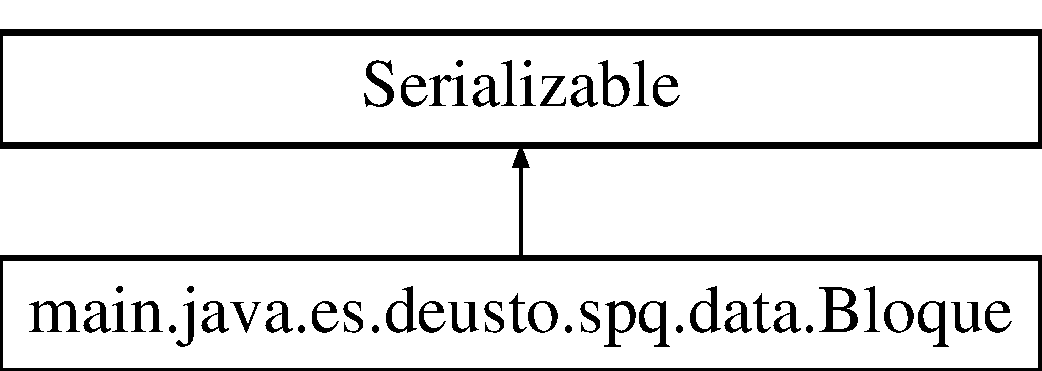
\includegraphics[height=2.000000cm]{classmain_1_1java_1_1es_1_1deusto_1_1spq_1_1data_1_1_bloque}
\end{center}
\end{figure}
\subsection*{Classes}
\begin{DoxyCompactItemize}
\item 
enum \hyperlink{enummain_1_1java_1_1es_1_1deusto_1_1spq_1_1data_1_1_bloque_1_1_tipo}{Tipo}
\end{DoxyCompactItemize}
\subsection*{Public Member Functions}
\begin{DoxyCompactItemize}
\item 
\hyperlink{classmain_1_1java_1_1es_1_1deusto_1_1spq_1_1data_1_1_bloque_a7b2e7048be726ab676f30aba17fd9525}{Bloque} (long tiempo, int pista, \hyperlink{enummain_1_1java_1_1es_1_1deusto_1_1spq_1_1data_1_1_bloque_1_1_tipo}{Tipo} tipo)
\item 
long \hyperlink{classmain_1_1java_1_1es_1_1deusto_1_1spq_1_1data_1_1_bloque_a07b95f7375eb215b787970b9ea2bf9a2}{get\+Tiempo} ()
\item 
void \hyperlink{classmain_1_1java_1_1es_1_1deusto_1_1spq_1_1data_1_1_bloque_a6b2064d83d0d4b7b29232c60768b9862}{set\+Tiempo} (long tiempo)
\item 
int \hyperlink{classmain_1_1java_1_1es_1_1deusto_1_1spq_1_1data_1_1_bloque_a2c1a9e5e23c1e02193c03bcb04d64d94}{get\+Pista} ()
\item 
void \hyperlink{classmain_1_1java_1_1es_1_1deusto_1_1spq_1_1data_1_1_bloque_a0cd770e3d3bbf78496bd2717f7f7b2e6}{set\+Pista} (int pista)
\item 
\hyperlink{enummain_1_1java_1_1es_1_1deusto_1_1spq_1_1data_1_1_bloque_1_1_tipo}{Tipo} \hyperlink{classmain_1_1java_1_1es_1_1deusto_1_1spq_1_1data_1_1_bloque_ad49cebd52cb2dcc25ac0d70a2a5fe28f}{get\+Tipo} ()
\item 
void \hyperlink{classmain_1_1java_1_1es_1_1deusto_1_1spq_1_1data_1_1_bloque_ae966d7da2545e1dff3ed02fc828933dc}{set\+Tipo} (\hyperlink{enummain_1_1java_1_1es_1_1deusto_1_1spq_1_1data_1_1_bloque_1_1_tipo}{Tipo} tipo)
\item 
void \hyperlink{classmain_1_1java_1_1es_1_1deusto_1_1spq_1_1data_1_1_bloque_a20587908c1aeede3bd189f441c268bf2}{quitar} ()
\end{DoxyCompactItemize}


\subsection{Detailed Description}
Clase para crear bloques con la informaci�n b�sica para el editor \begin{DoxyAuthor}{Author}
001 
\end{DoxyAuthor}


Definition at line 12 of file Bloque.\+java.



\subsection{Constructor \& Destructor Documentation}
\index{main\+::java\+::es\+::deusto\+::spq\+::data\+::\+Bloque@{main\+::java\+::es\+::deusto\+::spq\+::data\+::\+Bloque}!Bloque@{Bloque}}
\index{Bloque@{Bloque}!main\+::java\+::es\+::deusto\+::spq\+::data\+::\+Bloque@{main\+::java\+::es\+::deusto\+::spq\+::data\+::\+Bloque}}
\subsubsection[{\texorpdfstring{Bloque(long tiempo, int pista, Tipo tipo)}{Bloque(long tiempo, int pista, Tipo tipo)}}]{\setlength{\rightskip}{0pt plus 5cm}main.\+java.\+es.\+deusto.\+spq.\+data.\+Bloque.\+Bloque (
\begin{DoxyParamCaption}
\item[{long}]{tiempo, }
\item[{int}]{pista, }
\item[{{\bf Tipo}}]{tipo}
\end{DoxyParamCaption}
)}\hypertarget{classmain_1_1java_1_1es_1_1deusto_1_1spq_1_1data_1_1_bloque_a7b2e7048be726ab676f30aba17fd9525}{}\label{classmain_1_1java_1_1es_1_1deusto_1_1spq_1_1data_1_1_bloque_a7b2e7048be726ab676f30aba17fd9525}
Constructor de \hyperlink{classmain_1_1java_1_1es_1_1deusto_1_1spq_1_1data_1_1_bloque}{Bloque} 
\begin{DoxyParams}{Parameters}
{\em tiempo} & en el que aparece el bloque \\
\hline
{\em pista} & en la que aparece el bloque \\
\hline
{\em tipo} & de bloque \\
\hline
\end{DoxyParams}


Definition at line 24 of file Bloque.\+java.



\subsection{Member Function Documentation}
\index{main\+::java\+::es\+::deusto\+::spq\+::data\+::\+Bloque@{main\+::java\+::es\+::deusto\+::spq\+::data\+::\+Bloque}!get\+Pista@{get\+Pista}}
\index{get\+Pista@{get\+Pista}!main\+::java\+::es\+::deusto\+::spq\+::data\+::\+Bloque@{main\+::java\+::es\+::deusto\+::spq\+::data\+::\+Bloque}}
\subsubsection[{\texorpdfstring{get\+Pista()}{getPista()}}]{\setlength{\rightskip}{0pt plus 5cm}int main.\+java.\+es.\+deusto.\+spq.\+data.\+Bloque.\+get\+Pista (
\begin{DoxyParamCaption}
{}
\end{DoxyParamCaption}
)}\hypertarget{classmain_1_1java_1_1es_1_1deusto_1_1spq_1_1data_1_1_bloque_a2c1a9e5e23c1e02193c03bcb04d64d94}{}\label{classmain_1_1java_1_1es_1_1deusto_1_1spq_1_1data_1_1_bloque_a2c1a9e5e23c1e02193c03bcb04d64d94}
Devuelve la pista en la que se encuentra el bloque \begin{DoxyReturn}{Returns}
pista 
\end{DoxyReturn}


Definition at line 50 of file Bloque.\+java.

\index{main\+::java\+::es\+::deusto\+::spq\+::data\+::\+Bloque@{main\+::java\+::es\+::deusto\+::spq\+::data\+::\+Bloque}!get\+Tiempo@{get\+Tiempo}}
\index{get\+Tiempo@{get\+Tiempo}!main\+::java\+::es\+::deusto\+::spq\+::data\+::\+Bloque@{main\+::java\+::es\+::deusto\+::spq\+::data\+::\+Bloque}}
\subsubsection[{\texorpdfstring{get\+Tiempo()}{getTiempo()}}]{\setlength{\rightskip}{0pt plus 5cm}long main.\+java.\+es.\+deusto.\+spq.\+data.\+Bloque.\+get\+Tiempo (
\begin{DoxyParamCaption}
{}
\end{DoxyParamCaption}
)}\hypertarget{classmain_1_1java_1_1es_1_1deusto_1_1spq_1_1data_1_1_bloque_a07b95f7375eb215b787970b9ea2bf9a2}{}\label{classmain_1_1java_1_1es_1_1deusto_1_1spq_1_1data_1_1_bloque_a07b95f7375eb215b787970b9ea2bf9a2}
Devuelve el tiempo en el que aparece el bloque \begin{DoxyReturn}{Returns}
tiempo en el que aparece el bloque 
\end{DoxyReturn}


Definition at line 34 of file Bloque.\+java.

\index{main\+::java\+::es\+::deusto\+::spq\+::data\+::\+Bloque@{main\+::java\+::es\+::deusto\+::spq\+::data\+::\+Bloque}!get\+Tipo@{get\+Tipo}}
\index{get\+Tipo@{get\+Tipo}!main\+::java\+::es\+::deusto\+::spq\+::data\+::\+Bloque@{main\+::java\+::es\+::deusto\+::spq\+::data\+::\+Bloque}}
\subsubsection[{\texorpdfstring{get\+Tipo()}{getTipo()}}]{\setlength{\rightskip}{0pt plus 5cm}{\bf Tipo} main.\+java.\+es.\+deusto.\+spq.\+data.\+Bloque.\+get\+Tipo (
\begin{DoxyParamCaption}
{}
\end{DoxyParamCaption}
)}\hypertarget{classmain_1_1java_1_1es_1_1deusto_1_1spq_1_1data_1_1_bloque_ad49cebd52cb2dcc25ac0d70a2a5fe28f}{}\label{classmain_1_1java_1_1es_1_1deusto_1_1spq_1_1data_1_1_bloque_ad49cebd52cb2dcc25ac0d70a2a5fe28f}
Devuelve el tipo de bloque \begin{DoxyReturn}{Returns}
tipo 
\end{DoxyReturn}


Definition at line 66 of file Bloque.\+java.

\index{main\+::java\+::es\+::deusto\+::spq\+::data\+::\+Bloque@{main\+::java\+::es\+::deusto\+::spq\+::data\+::\+Bloque}!quitar@{quitar}}
\index{quitar@{quitar}!main\+::java\+::es\+::deusto\+::spq\+::data\+::\+Bloque@{main\+::java\+::es\+::deusto\+::spq\+::data\+::\+Bloque}}
\subsubsection[{\texorpdfstring{quitar()}{quitar()}}]{\setlength{\rightskip}{0pt plus 5cm}void main.\+java.\+es.\+deusto.\+spq.\+data.\+Bloque.\+quitar (
\begin{DoxyParamCaption}
{}
\end{DoxyParamCaption}
)}\hypertarget{classmain_1_1java_1_1es_1_1deusto_1_1spq_1_1data_1_1_bloque_a20587908c1aeede3bd189f441c268bf2}{}\label{classmain_1_1java_1_1es_1_1deusto_1_1spq_1_1data_1_1_bloque_a20587908c1aeede3bd189f441c268bf2}


Definition at line 88 of file Bloque.\+java.

\index{main\+::java\+::es\+::deusto\+::spq\+::data\+::\+Bloque@{main\+::java\+::es\+::deusto\+::spq\+::data\+::\+Bloque}!set\+Pista@{set\+Pista}}
\index{set\+Pista@{set\+Pista}!main\+::java\+::es\+::deusto\+::spq\+::data\+::\+Bloque@{main\+::java\+::es\+::deusto\+::spq\+::data\+::\+Bloque}}
\subsubsection[{\texorpdfstring{set\+Pista(int pista)}{setPista(int pista)}}]{\setlength{\rightskip}{0pt plus 5cm}void main.\+java.\+es.\+deusto.\+spq.\+data.\+Bloque.\+set\+Pista (
\begin{DoxyParamCaption}
\item[{int}]{pista}
\end{DoxyParamCaption}
)}\hypertarget{classmain_1_1java_1_1es_1_1deusto_1_1spq_1_1data_1_1_bloque_a0cd770e3d3bbf78496bd2717f7f7b2e6}{}\label{classmain_1_1java_1_1es_1_1deusto_1_1spq_1_1data_1_1_bloque_a0cd770e3d3bbf78496bd2717f7f7b2e6}
Establece la pista en la que se encuentra el bloque 
\begin{DoxyParams}{Parameters}
{\em pista} & a establecer \\
\hline
\end{DoxyParams}


Definition at line 58 of file Bloque.\+java.

\index{main\+::java\+::es\+::deusto\+::spq\+::data\+::\+Bloque@{main\+::java\+::es\+::deusto\+::spq\+::data\+::\+Bloque}!set\+Tiempo@{set\+Tiempo}}
\index{set\+Tiempo@{set\+Tiempo}!main\+::java\+::es\+::deusto\+::spq\+::data\+::\+Bloque@{main\+::java\+::es\+::deusto\+::spq\+::data\+::\+Bloque}}
\subsubsection[{\texorpdfstring{set\+Tiempo(long tiempo)}{setTiempo(long tiempo)}}]{\setlength{\rightskip}{0pt plus 5cm}void main.\+java.\+es.\+deusto.\+spq.\+data.\+Bloque.\+set\+Tiempo (
\begin{DoxyParamCaption}
\item[{long}]{tiempo}
\end{DoxyParamCaption}
)}\hypertarget{classmain_1_1java_1_1es_1_1deusto_1_1spq_1_1data_1_1_bloque_a6b2064d83d0d4b7b29232c60768b9862}{}\label{classmain_1_1java_1_1es_1_1deusto_1_1spq_1_1data_1_1_bloque_a6b2064d83d0d4b7b29232c60768b9862}
Establece el tiempo en que aparece el bloque 
\begin{DoxyParams}{Parameters}
{\em tiempo} & a establecer \\
\hline
\end{DoxyParams}


Definition at line 42 of file Bloque.\+java.

\index{main\+::java\+::es\+::deusto\+::spq\+::data\+::\+Bloque@{main\+::java\+::es\+::deusto\+::spq\+::data\+::\+Bloque}!set\+Tipo@{set\+Tipo}}
\index{set\+Tipo@{set\+Tipo}!main\+::java\+::es\+::deusto\+::spq\+::data\+::\+Bloque@{main\+::java\+::es\+::deusto\+::spq\+::data\+::\+Bloque}}
\subsubsection[{\texorpdfstring{set\+Tipo(\+Tipo tipo)}{setTipo(Tipo tipo)}}]{\setlength{\rightskip}{0pt plus 5cm}void main.\+java.\+es.\+deusto.\+spq.\+data.\+Bloque.\+set\+Tipo (
\begin{DoxyParamCaption}
\item[{{\bf Tipo}}]{tipo}
\end{DoxyParamCaption}
)}\hypertarget{classmain_1_1java_1_1es_1_1deusto_1_1spq_1_1data_1_1_bloque_ae966d7da2545e1dff3ed02fc828933dc}{}\label{classmain_1_1java_1_1es_1_1deusto_1_1spq_1_1data_1_1_bloque_ae966d7da2545e1dff3ed02fc828933dc}
Establece el tipo de bloque 
\begin{DoxyParams}{Parameters}
{\em tipo} & de bloque a establecer \\
\hline
\end{DoxyParams}


Definition at line 74 of file Bloque.\+java.



The documentation for this class was generated from the following file\+:\begin{DoxyCompactItemize}
\item 
src/main/java/es/deusto/spq/data/\hyperlink{_bloque_8java}{Bloque.\+java}\end{DoxyCompactItemize}

\hypertarget{classmain_1_1java_1_1es_1_1deusto_1_1spq_1_1data_1_1_bloque_grafico}{}\section{main.\+java.\+es.\+deusto.\+spq.\+data.\+Bloque\+Grafico Class Reference}
\label{classmain_1_1java_1_1es_1_1deusto_1_1spq_1_1data_1_1_bloque_grafico}\index{main.\+java.\+es.\+deusto.\+spq.\+data.\+Bloque\+Grafico@{main.\+java.\+es.\+deusto.\+spq.\+data.\+Bloque\+Grafico}}
Inheritance diagram for main.\+java.\+es.\+deusto.\+spq.\+data.\+Bloque\+Grafico\+:\begin{figure}[H]
\begin{center}
\leavevmode
\includegraphics[height=3.000000cm]{classmain_1_1java_1_1es_1_1deusto_1_1spq_1_1data_1_1_bloque_grafico}
\end{center}
\end{figure}
\subsection*{Public Member Functions}
\begin{DoxyCompactItemize}
\item 
\hyperlink{classmain_1_1java_1_1es_1_1deusto_1_1spq_1_1data_1_1_bloque_grafico_a69517caff67216c3ad78e0208bf45b51}{Bloque\+Grafico} (\hyperlink{classmain_1_1java_1_1es_1_1deusto_1_1spq_1_1data_1_1_bloque}{Bloque} b, String \hyperlink{classmain_1_1java_1_1es_1_1deusto_1_1spq_1_1windows_1_1_objeto_grafico_aaf5e1e8c4ebff8a39c72b07c8af6ca86}{nombre\+Imagen\+Objeto}, boolean visible)
\item 
int \hyperlink{classmain_1_1java_1_1es_1_1deusto_1_1spq_1_1data_1_1_bloque_grafico_a3b3246f25d904795805a35077736b401}{get\+PosX} ()
\item 
int \hyperlink{classmain_1_1java_1_1es_1_1deusto_1_1spq_1_1data_1_1_bloque_grafico_a8e7a3b1859ea6b3f2040323438c82ef6}{get\+PosY} ()
\item 
void \hyperlink{classmain_1_1java_1_1es_1_1deusto_1_1spq_1_1data_1_1_bloque_grafico_aaf8e5ff1114f980102c03f3215a508c1}{set\+PosY} (int posY)
\item 
\hyperlink{classmain_1_1java_1_1es_1_1deusto_1_1spq_1_1data_1_1_bloque}{Bloque} \hyperlink{classmain_1_1java_1_1es_1_1deusto_1_1spq_1_1data_1_1_bloque_grafico_a11b4f4a371cbe47cd5ddbb2718925a92}{get\+Bloque} ()
\item 
\hyperlink{classmain_1_1java_1_1es_1_1deusto_1_1spq_1_1windows_1_1_objeto_grafico}{Objeto\+Grafico} \hyperlink{classmain_1_1java_1_1es_1_1deusto_1_1spq_1_1data_1_1_bloque_grafico_a93c7c8717111e871aa234fd047c76ca5}{get\+Objeto} ()
\end{DoxyCompactItemize}
\subsection*{Additional Inherited Members}


\subsection{Detailed Description}
Clase para crear un bloque que aparece por pantalla \begin{DoxyAuthor}{Author}
001 
\end{DoxyAuthor}


Definition at line 10 of file Bloque\+Grafico.\+java.



\subsection{Constructor \& Destructor Documentation}
\index{main\+::java\+::es\+::deusto\+::spq\+::data\+::\+Bloque\+Grafico@{main\+::java\+::es\+::deusto\+::spq\+::data\+::\+Bloque\+Grafico}!Bloque\+Grafico@{Bloque\+Grafico}}
\index{Bloque\+Grafico@{Bloque\+Grafico}!main\+::java\+::es\+::deusto\+::spq\+::data\+::\+Bloque\+Grafico@{main\+::java\+::es\+::deusto\+::spq\+::data\+::\+Bloque\+Grafico}}
\subsubsection[{\texorpdfstring{Bloque\+Grafico(\+Bloque b, String nombre\+Imagen\+Objeto, boolean visible)}{BloqueGrafico(Bloque b, String nombreImagenObjeto, boolean visible)}}]{\setlength{\rightskip}{0pt plus 5cm}main.\+java.\+es.\+deusto.\+spq.\+data.\+Bloque\+Grafico.\+Bloque\+Grafico (
\begin{DoxyParamCaption}
\item[{{\bf Bloque}}]{b, }
\item[{String}]{nombre\+Imagen\+Objeto, }
\item[{boolean}]{visible}
\end{DoxyParamCaption}
)}\hypertarget{classmain_1_1java_1_1es_1_1deusto_1_1spq_1_1data_1_1_bloque_grafico_a69517caff67216c3ad78e0208bf45b51}{}\label{classmain_1_1java_1_1es_1_1deusto_1_1spq_1_1data_1_1_bloque_grafico_a69517caff67216c3ad78e0208bf45b51}
Constructor para crear un bloque gr�fico 
\begin{DoxyParams}{Parameters}
{\em b} & bloque con los datos de tiempo, pista y tipo \\
\hline
{\em nombre\+Imagen\+Objeto} & nombre del fichero de imagen del objeto \\
\hline
{\em visible} & si es visible por pantalla o no \\
\hline
\end{DoxyParams}


Definition at line 24 of file Bloque\+Grafico.\+java.



\subsection{Member Function Documentation}
\index{main\+::java\+::es\+::deusto\+::spq\+::data\+::\+Bloque\+Grafico@{main\+::java\+::es\+::deusto\+::spq\+::data\+::\+Bloque\+Grafico}!get\+Bloque@{get\+Bloque}}
\index{get\+Bloque@{get\+Bloque}!main\+::java\+::es\+::deusto\+::spq\+::data\+::\+Bloque\+Grafico@{main\+::java\+::es\+::deusto\+::spq\+::data\+::\+Bloque\+Grafico}}
\subsubsection[{\texorpdfstring{get\+Bloque()}{getBloque()}}]{\setlength{\rightskip}{0pt plus 5cm}{\bf Bloque} main.\+java.\+es.\+deusto.\+spq.\+data.\+Bloque\+Grafico.\+get\+Bloque (
\begin{DoxyParamCaption}
{}
\end{DoxyParamCaption}
)}\hypertarget{classmain_1_1java_1_1es_1_1deusto_1_1spq_1_1data_1_1_bloque_grafico_a11b4f4a371cbe47cd5ddbb2718925a92}{}\label{classmain_1_1java_1_1es_1_1deusto_1_1spq_1_1data_1_1_bloque_grafico_a11b4f4a371cbe47cd5ddbb2718925a92}
Devuelve el objeto bloque dentro de un bloque gr�fico \begin{DoxyReturn}{Returns}
b bloque 
\end{DoxyReturn}


Definition at line 75 of file Bloque\+Grafico.\+java.

\index{main\+::java\+::es\+::deusto\+::spq\+::data\+::\+Bloque\+Grafico@{main\+::java\+::es\+::deusto\+::spq\+::data\+::\+Bloque\+Grafico}!get\+Objeto@{get\+Objeto}}
\index{get\+Objeto@{get\+Objeto}!main\+::java\+::es\+::deusto\+::spq\+::data\+::\+Bloque\+Grafico@{main\+::java\+::es\+::deusto\+::spq\+::data\+::\+Bloque\+Grafico}}
\subsubsection[{\texorpdfstring{get\+Objeto()}{getObjeto()}}]{\setlength{\rightskip}{0pt plus 5cm}{\bf Objeto\+Grafico} main.\+java.\+es.\+deusto.\+spq.\+data.\+Bloque\+Grafico.\+get\+Objeto (
\begin{DoxyParamCaption}
{}
\end{DoxyParamCaption}
)}\hypertarget{classmain_1_1java_1_1es_1_1deusto_1_1spq_1_1data_1_1_bloque_grafico_a93c7c8717111e871aa234fd047c76ca5}{}\label{classmain_1_1java_1_1es_1_1deusto_1_1spq_1_1data_1_1_bloque_grafico_a93c7c8717111e871aa234fd047c76ca5}
Devuelve el objeto gr�fico de este bloque gr�fico \begin{DoxyReturn}{Returns}
Objeto gr�fico de este bloque 
\end{DoxyReturn}


Definition at line 83 of file Bloque\+Grafico.\+java.

\index{main\+::java\+::es\+::deusto\+::spq\+::data\+::\+Bloque\+Grafico@{main\+::java\+::es\+::deusto\+::spq\+::data\+::\+Bloque\+Grafico}!get\+PosX@{get\+PosX}}
\index{get\+PosX@{get\+PosX}!main\+::java\+::es\+::deusto\+::spq\+::data\+::\+Bloque\+Grafico@{main\+::java\+::es\+::deusto\+::spq\+::data\+::\+Bloque\+Grafico}}
\subsubsection[{\texorpdfstring{get\+Pos\+X()}{getPosX()}}]{\setlength{\rightskip}{0pt plus 5cm}int main.\+java.\+es.\+deusto.\+spq.\+data.\+Bloque\+Grafico.\+get\+PosX (
\begin{DoxyParamCaption}
{}
\end{DoxyParamCaption}
)}\hypertarget{classmain_1_1java_1_1es_1_1deusto_1_1spq_1_1data_1_1_bloque_grafico_a3b3246f25d904795805a35077736b401}{}\label{classmain_1_1java_1_1es_1_1deusto_1_1spq_1_1data_1_1_bloque_grafico_a3b3246f25d904795805a35077736b401}
Devuelve la posici�n x del bloque \begin{DoxyReturn}{Returns}
posX posici�n del bloque gr�fico 
\end{DoxyReturn}


Definition at line 51 of file Bloque\+Grafico.\+java.

\index{main\+::java\+::es\+::deusto\+::spq\+::data\+::\+Bloque\+Grafico@{main\+::java\+::es\+::deusto\+::spq\+::data\+::\+Bloque\+Grafico}!get\+PosY@{get\+PosY}}
\index{get\+PosY@{get\+PosY}!main\+::java\+::es\+::deusto\+::spq\+::data\+::\+Bloque\+Grafico@{main\+::java\+::es\+::deusto\+::spq\+::data\+::\+Bloque\+Grafico}}
\subsubsection[{\texorpdfstring{get\+Pos\+Y()}{getPosY()}}]{\setlength{\rightskip}{0pt plus 5cm}int main.\+java.\+es.\+deusto.\+spq.\+data.\+Bloque\+Grafico.\+get\+PosY (
\begin{DoxyParamCaption}
{}
\end{DoxyParamCaption}
)}\hypertarget{classmain_1_1java_1_1es_1_1deusto_1_1spq_1_1data_1_1_bloque_grafico_a8e7a3b1859ea6b3f2040323438c82ef6}{}\label{classmain_1_1java_1_1es_1_1deusto_1_1spq_1_1data_1_1_bloque_grafico_a8e7a3b1859ea6b3f2040323438c82ef6}
Devuelve la posici�n y del bloque \begin{DoxyReturn}{Returns}
posY posici�n y del bloque gr�fico 
\end{DoxyReturn}


Definition at line 59 of file Bloque\+Grafico.\+java.

\index{main\+::java\+::es\+::deusto\+::spq\+::data\+::\+Bloque\+Grafico@{main\+::java\+::es\+::deusto\+::spq\+::data\+::\+Bloque\+Grafico}!set\+PosY@{set\+PosY}}
\index{set\+PosY@{set\+PosY}!main\+::java\+::es\+::deusto\+::spq\+::data\+::\+Bloque\+Grafico@{main\+::java\+::es\+::deusto\+::spq\+::data\+::\+Bloque\+Grafico}}
\subsubsection[{\texorpdfstring{set\+Pos\+Y(int pos\+Y)}{setPosY(int posY)}}]{\setlength{\rightskip}{0pt plus 5cm}void main.\+java.\+es.\+deusto.\+spq.\+data.\+Bloque\+Grafico.\+set\+PosY (
\begin{DoxyParamCaption}
\item[{int}]{posY}
\end{DoxyParamCaption}
)}\hypertarget{classmain_1_1java_1_1es_1_1deusto_1_1spq_1_1data_1_1_bloque_grafico_aaf8e5ff1114f980102c03f3215a508c1}{}\label{classmain_1_1java_1_1es_1_1deusto_1_1spq_1_1data_1_1_bloque_grafico_aaf8e5ff1114f980102c03f3215a508c1}
Establece la posici�n y del bloque 
\begin{DoxyParams}{Parameters}
{\em posY} & posici�n y del bloque gr�fico \\
\hline
\end{DoxyParams}


Definition at line 67 of file Bloque\+Grafico.\+java.



The documentation for this class was generated from the following file\+:\begin{DoxyCompactItemize}
\item 
src/main/java/es/deusto/spq/data/\hyperlink{_bloque_grafico_8java}{Bloque\+Grafico.\+java}\end{DoxyCompactItemize}

\hypertarget{classmain_1_1java_1_1es_1_1deusto_1_1spq_1_1data_1_1_cancion}{}\section{main.\+java.\+es.\+deusto.\+spq.\+data.\+Cancion Class Reference}
\label{classmain_1_1java_1_1es_1_1deusto_1_1spq_1_1data_1_1_cancion}\index{main.\+java.\+es.\+deusto.\+spq.\+data.\+Cancion@{main.\+java.\+es.\+deusto.\+spq.\+data.\+Cancion}}
\subsection*{Public Member Functions}
\begin{DoxyCompactItemize}
\item 
\hyperlink{classmain_1_1java_1_1es_1_1deusto_1_1spq_1_1data_1_1_cancion_a378e14b5f95bad5189b50f57ec5ef475}{Cancion} (String titulo, String dir)
\item 
String \hyperlink{classmain_1_1java_1_1es_1_1deusto_1_1spq_1_1data_1_1_cancion_ad3d7b1cfcea3c4c3107feb8082e4bdf5}{get\+Titulo} ()
\item 
String \hyperlink{classmain_1_1java_1_1es_1_1deusto_1_1spq_1_1data_1_1_cancion_a12e64089a8fd660fcea838b96c0cd649}{get\+Dir} ()
\end{DoxyCompactItemize}


\subsection{Detailed Description}
Clase para crear objetos de tipo canci�n \begin{DoxyAuthor}{Author}
001 
\end{DoxyAuthor}


Definition at line 8 of file Cancion.\+java.



\subsection{Constructor \& Destructor Documentation}
\index{main\+::java\+::es\+::deusto\+::spq\+::data\+::\+Cancion@{main\+::java\+::es\+::deusto\+::spq\+::data\+::\+Cancion}!Cancion@{Cancion}}
\index{Cancion@{Cancion}!main\+::java\+::es\+::deusto\+::spq\+::data\+::\+Cancion@{main\+::java\+::es\+::deusto\+::spq\+::data\+::\+Cancion}}
\subsubsection[{\texorpdfstring{Cancion(\+String titulo, String dir)}{Cancion(String titulo, String dir)}}]{\setlength{\rightskip}{0pt plus 5cm}main.\+java.\+es.\+deusto.\+spq.\+data.\+Cancion.\+Cancion (
\begin{DoxyParamCaption}
\item[{String}]{titulo, }
\item[{String}]{dir}
\end{DoxyParamCaption}
)}\hypertarget{classmain_1_1java_1_1es_1_1deusto_1_1spq_1_1data_1_1_cancion_a378e14b5f95bad5189b50f57ec5ef475}{}\label{classmain_1_1java_1_1es_1_1deusto_1_1spq_1_1data_1_1_cancion_a378e14b5f95bad5189b50f57ec5ef475}
Constructor de la clase Canci�n 
\begin{DoxyParams}{Parameters}
{\em titulo} & de la canci�n \\
\hline
{\em dir} & direcci�n del archivo \\
\hline
{\em p\+Max} & puntuaci�n m�xima sacada en la canci�n \\
\hline
\end{DoxyParams}


Definition at line 18 of file Cancion.\+java.



\subsection{Member Function Documentation}
\index{main\+::java\+::es\+::deusto\+::spq\+::data\+::\+Cancion@{main\+::java\+::es\+::deusto\+::spq\+::data\+::\+Cancion}!get\+Dir@{get\+Dir}}
\index{get\+Dir@{get\+Dir}!main\+::java\+::es\+::deusto\+::spq\+::data\+::\+Cancion@{main\+::java\+::es\+::deusto\+::spq\+::data\+::\+Cancion}}
\subsubsection[{\texorpdfstring{get\+Dir()}{getDir()}}]{\setlength{\rightskip}{0pt plus 5cm}String main.\+java.\+es.\+deusto.\+spq.\+data.\+Cancion.\+get\+Dir (
\begin{DoxyParamCaption}
{}
\end{DoxyParamCaption}
)}\hypertarget{classmain_1_1java_1_1es_1_1deusto_1_1spq_1_1data_1_1_cancion_a12e64089a8fd660fcea838b96c0cd649}{}\label{classmain_1_1java_1_1es_1_1deusto_1_1spq_1_1data_1_1_cancion_a12e64089a8fd660fcea838b96c0cd649}
Devuelve la direcci�n del archivo \begin{DoxyReturn}{Returns}
direcci�n del archivo 
\end{DoxyReturn}


Definition at line 36 of file Cancion.\+java.

\index{main\+::java\+::es\+::deusto\+::spq\+::data\+::\+Cancion@{main\+::java\+::es\+::deusto\+::spq\+::data\+::\+Cancion}!get\+Titulo@{get\+Titulo}}
\index{get\+Titulo@{get\+Titulo}!main\+::java\+::es\+::deusto\+::spq\+::data\+::\+Cancion@{main\+::java\+::es\+::deusto\+::spq\+::data\+::\+Cancion}}
\subsubsection[{\texorpdfstring{get\+Titulo()}{getTitulo()}}]{\setlength{\rightskip}{0pt plus 5cm}String main.\+java.\+es.\+deusto.\+spq.\+data.\+Cancion.\+get\+Titulo (
\begin{DoxyParamCaption}
{}
\end{DoxyParamCaption}
)}\hypertarget{classmain_1_1java_1_1es_1_1deusto_1_1spq_1_1data_1_1_cancion_ad3d7b1cfcea3c4c3107feb8082e4bdf5}{}\label{classmain_1_1java_1_1es_1_1deusto_1_1spq_1_1data_1_1_cancion_ad3d7b1cfcea3c4c3107feb8082e4bdf5}
Devuelve el t�tulo de la canci�n \begin{DoxyReturn}{Returns}
titulo de la canci�n 
\end{DoxyReturn}


Definition at line 28 of file Cancion.\+java.



The documentation for this class was generated from the following file\+:\begin{DoxyCompactItemize}
\item 
src/main/java/es/deusto/spq/data/\hyperlink{_cancion_8java}{Cancion.\+java}\end{DoxyCompactItemize}

\hypertarget{classmain_1_1java_1_1es_1_1deusto_1_1spq_1_1utils_1_1_file_manager}{}\section{main.\+java.\+es.\+deusto.\+spq.\+utils.\+File\+Manager Class Reference}
\label{classmain_1_1java_1_1es_1_1deusto_1_1spq_1_1utils_1_1_file_manager}\index{main.\+java.\+es.\+deusto.\+spq.\+utils.\+File\+Manager@{main.\+java.\+es.\+deusto.\+spq.\+utils.\+File\+Manager}}
\subsection*{Static Public Member Functions}
\begin{DoxyCompactItemize}
\item 
static void \hyperlink{classmain_1_1java_1_1es_1_1deusto_1_1spq_1_1utils_1_1_file_manager_aaa99c5afe5162e5964859f6caf95cbae}{save\+Bloque\+To\+File} (Array\+List$<$ \hyperlink{classmain_1_1java_1_1es_1_1deusto_1_1spq_1_1data_1_1_bloque}{Bloque} $>$ lista\+Bloques\+Guardar, String titulo)  throws File\+Not\+Found\+Exception, I\+O\+Exception 
\item 
static Array\+List$<$ \hyperlink{classmain_1_1java_1_1es_1_1deusto_1_1spq_1_1data_1_1_bloque}{Bloque} $>$ \hyperlink{classmain_1_1java_1_1es_1_1deusto_1_1spq_1_1utils_1_1_file_manager_a202c7743f2fb4b3d2bfc1cd2cafdd06e}{read\+Bloque\+From\+File} (String titulo)  throws Exception 
\item 
static void \hyperlink{classmain_1_1java_1_1es_1_1deusto_1_1spq_1_1utils_1_1_file_manager_ae5e7b717e8cc0c81f3109c702f10ff40}{file\+Copy} (String source\+File, String destination\+File)
\end{DoxyCompactItemize}


\subsection{Detailed Description}
Clase para el manejo de ficheros \begin{DoxyAuthor}{Author}
001 
\end{DoxyAuthor}


Definition at line 12 of file File\+Manager.\+java.



\subsection{Member Function Documentation}
\index{main\+::java\+::es\+::deusto\+::spq\+::utils\+::\+File\+Manager@{main\+::java\+::es\+::deusto\+::spq\+::utils\+::\+File\+Manager}!file\+Copy@{file\+Copy}}
\index{file\+Copy@{file\+Copy}!main\+::java\+::es\+::deusto\+::spq\+::utils\+::\+File\+Manager@{main\+::java\+::es\+::deusto\+::spq\+::utils\+::\+File\+Manager}}
\subsubsection[{\texorpdfstring{file\+Copy(\+String source\+File, String destination\+File)}{fileCopy(String sourceFile, String destinationFile)}}]{\setlength{\rightskip}{0pt plus 5cm}static void main.\+java.\+es.\+deusto.\+spq.\+utils.\+File\+Manager.\+file\+Copy (
\begin{DoxyParamCaption}
\item[{String}]{source\+File, }
\item[{String}]{destination\+File}
\end{DoxyParamCaption}
)\hspace{0.3cm}{\ttfamily [static]}}\hypertarget{classmain_1_1java_1_1es_1_1deusto_1_1spq_1_1utils_1_1_file_manager_ae5e7b717e8cc0c81f3109c702f10ff40}{}\label{classmain_1_1java_1_1es_1_1deusto_1_1spq_1_1utils_1_1_file_manager_ae5e7b717e8cc0c81f3109c702f10ff40}
Copia un fichero en otro lugar 
\begin{DoxyParams}{Parameters}
{\em source\+File} & ruta del fichero original \\
\hline
{\em destination\+File} & ruta a la que copiamos el fichero \\
\hline
\end{DoxyParams}


Definition at line 48 of file File\+Manager.\+java.

\index{main\+::java\+::es\+::deusto\+::spq\+::utils\+::\+File\+Manager@{main\+::java\+::es\+::deusto\+::spq\+::utils\+::\+File\+Manager}!read\+Bloque\+From\+File@{read\+Bloque\+From\+File}}
\index{read\+Bloque\+From\+File@{read\+Bloque\+From\+File}!main\+::java\+::es\+::deusto\+::spq\+::utils\+::\+File\+Manager@{main\+::java\+::es\+::deusto\+::spq\+::utils\+::\+File\+Manager}}
\subsubsection[{\texorpdfstring{read\+Bloque\+From\+File(\+String titulo)}{readBloqueFromFile(String titulo)}}]{\setlength{\rightskip}{0pt plus 5cm}static Array\+List$<${\bf Bloque}$>$ main.\+java.\+es.\+deusto.\+spq.\+utils.\+File\+Manager.\+read\+Bloque\+From\+File (
\begin{DoxyParamCaption}
\item[{String}]{titulo}
\end{DoxyParamCaption}
) throws Exception\hspace{0.3cm}{\ttfamily [static]}}\hypertarget{classmain_1_1java_1_1es_1_1deusto_1_1spq_1_1utils_1_1_file_manager_a202c7743f2fb4b3d2bfc1cd2cafdd06e}{}\label{classmain_1_1java_1_1es_1_1deusto_1_1spq_1_1utils_1_1_file_manager_a202c7743f2fb4b3d2bfc1cd2cafdd06e}
Carga un fichero que tiene objetos de tipo bloque 
\begin{DoxyParams}{Parameters}
{\em titulo} & nombre del fichero a cargar \\
\hline
\end{DoxyParams}
\begin{DoxyReturn}{Returns}
arraylist de bloques 
\end{DoxyReturn}

\begin{DoxyExceptions}{Exceptions}
{\em Exception} & \\
\hline
\end{DoxyExceptions}


Definition at line 35 of file File\+Manager.\+java.

\index{main\+::java\+::es\+::deusto\+::spq\+::utils\+::\+File\+Manager@{main\+::java\+::es\+::deusto\+::spq\+::utils\+::\+File\+Manager}!save\+Bloque\+To\+File@{save\+Bloque\+To\+File}}
\index{save\+Bloque\+To\+File@{save\+Bloque\+To\+File}!main\+::java\+::es\+::deusto\+::spq\+::utils\+::\+File\+Manager@{main\+::java\+::es\+::deusto\+::spq\+::utils\+::\+File\+Manager}}
\subsubsection[{\texorpdfstring{save\+Bloque\+To\+File(\+Array\+List$<$ Bloque $>$ lista\+Bloques\+Guardar, String titulo)}{saveBloqueToFile(ArrayList< Bloque > listaBloquesGuardar, String titulo)}}]{\setlength{\rightskip}{0pt plus 5cm}static void main.\+java.\+es.\+deusto.\+spq.\+utils.\+File\+Manager.\+save\+Bloque\+To\+File (
\begin{DoxyParamCaption}
\item[{Array\+List$<$ {\bf Bloque} $>$}]{lista\+Bloques\+Guardar, }
\item[{String}]{titulo}
\end{DoxyParamCaption}
) throws File\+Not\+Found\+Exception, I\+O\+Exception\hspace{0.3cm}{\ttfamily [static]}}\hypertarget{classmain_1_1java_1_1es_1_1deusto_1_1spq_1_1utils_1_1_file_manager_aaa99c5afe5162e5964859f6caf95cbae}{}\label{classmain_1_1java_1_1es_1_1deusto_1_1spq_1_1utils_1_1_file_manager_aaa99c5afe5162e5964859f6caf95cbae}
Guarda un fichero con objetos de tipo bloque 
\begin{DoxyParams}{Parameters}
{\em lista\+Bloques\+Guardar} & arraylist de tipo bloque, es lo que se guarda \\
\hline
{\em titulo} & nombre del fichero \\
\hline
\end{DoxyParams}

\begin{DoxyExceptions}{Exceptions}
{\em File\+Not\+Found\+Exception} & \\
\hline
{\em I\+O\+Exception} & \\
\hline
\end{DoxyExceptions}


Definition at line 21 of file File\+Manager.\+java.



The documentation for this class was generated from the following file\+:\begin{DoxyCompactItemize}
\item 
src/main/java/es/deusto/spq/utils/\hyperlink{_file_manager_8java}{File\+Manager.\+java}\end{DoxyCompactItemize}

\hypertarget{classmain_1_1java_1_1es_1_1deusto_1_1spq_1_1windows_1_1_menu_window}{}\section{main.\+java.\+es.\+deusto.\+spq.\+windows.\+Menu\+Window Class Reference}
\label{classmain_1_1java_1_1es_1_1deusto_1_1spq_1_1windows_1_1_menu_window}\index{main.\+java.\+es.\+deusto.\+spq.\+windows.\+Menu\+Window@{main.\+java.\+es.\+deusto.\+spq.\+windows.\+Menu\+Window}}
Inheritance diagram for main.\+java.\+es.\+deusto.\+spq.\+windows.\+Menu\+Window\+:\begin{figure}[H]
\begin{center}
\leavevmode
\includegraphics[height=1.951219cm]{classmain_1_1java_1_1es_1_1deusto_1_1spq_1_1windows_1_1_menu_window}
\end{center}
\end{figure}
\subsection*{Classes}
\begin{DoxyCompactItemize}
\item 
class {\bfseries Quit}
\end{DoxyCompactItemize}
\subsection*{Public Member Functions}
\begin{DoxyCompactItemize}
\item 
\hyperlink{classmain_1_1java_1_1es_1_1deusto_1_1spq_1_1windows_1_1_menu_window_a873f49767242873a6267f460dcf0f41d}{Menu\+Window} ()
\item 
void \hyperlink{classmain_1_1java_1_1es_1_1deusto_1_1spq_1_1windows_1_1_menu_window_a03b991737dc73a911d888d114e57656b}{action\+Performed} (Action\+Event arg0)
\end{DoxyCompactItemize}
\subsection*{Static Public Member Functions}
\begin{DoxyCompactItemize}
\item 
static void \hyperlink{classmain_1_1java_1_1es_1_1deusto_1_1spq_1_1windows_1_1_menu_window_a4f4ad79d75c1fe7fa91cd8bb42e199b3}{main} (String\mbox{[}$\,$\mbox{]} args)
\end{DoxyCompactItemize}


\subsection{Detailed Description}
Clase que crea la ventana del menu de juego \begin{DoxyAuthor}{Author}
001 
\end{DoxyAuthor}


Definition at line 35 of file Menu\+Window.\+java.



\subsection{Constructor \& Destructor Documentation}
\index{main\+::java\+::es\+::deusto\+::spq\+::windows\+::\+Menu\+Window@{main\+::java\+::es\+::deusto\+::spq\+::windows\+::\+Menu\+Window}!Menu\+Window@{Menu\+Window}}
\index{Menu\+Window@{Menu\+Window}!main\+::java\+::es\+::deusto\+::spq\+::windows\+::\+Menu\+Window@{main\+::java\+::es\+::deusto\+::spq\+::windows\+::\+Menu\+Window}}
\subsubsection[{\texorpdfstring{Menu\+Window()}{MenuWindow()}}]{\setlength{\rightskip}{0pt plus 5cm}main.\+java.\+es.\+deusto.\+spq.\+windows.\+Menu\+Window.\+Menu\+Window (
\begin{DoxyParamCaption}
{}
\end{DoxyParamCaption}
)}\hypertarget{classmain_1_1java_1_1es_1_1deusto_1_1spq_1_1windows_1_1_menu_window_a873f49767242873a6267f460dcf0f41d}{}\label{classmain_1_1java_1_1es_1_1deusto_1_1spq_1_1windows_1_1_menu_window_a873f49767242873a6267f460dcf0f41d}
Constructor de la ventana 

Definition at line 65 of file Menu\+Window.\+java.



\subsection{Member Function Documentation}
\index{main\+::java\+::es\+::deusto\+::spq\+::windows\+::\+Menu\+Window@{main\+::java\+::es\+::deusto\+::spq\+::windows\+::\+Menu\+Window}!action\+Performed@{action\+Performed}}
\index{action\+Performed@{action\+Performed}!main\+::java\+::es\+::deusto\+::spq\+::windows\+::\+Menu\+Window@{main\+::java\+::es\+::deusto\+::spq\+::windows\+::\+Menu\+Window}}
\subsubsection[{\texorpdfstring{action\+Performed(\+Action\+Event arg0)}{actionPerformed(ActionEvent arg0)}}]{\setlength{\rightskip}{0pt plus 5cm}void main.\+java.\+es.\+deusto.\+spq.\+windows.\+Menu\+Window.\+action\+Performed (
\begin{DoxyParamCaption}
\item[{Action\+Event}]{arg0}
\end{DoxyParamCaption}
)}\hypertarget{classmain_1_1java_1_1es_1_1deusto_1_1spq_1_1windows_1_1_menu_window_a03b991737dc73a911d888d114e57656b}{}\label{classmain_1_1java_1_1es_1_1deusto_1_1spq_1_1windows_1_1_menu_window_a03b991737dc73a911d888d114e57656b}
M�todo del action\+Listener 

Definition at line 143 of file Menu\+Window.\+java.

\index{main\+::java\+::es\+::deusto\+::spq\+::windows\+::\+Menu\+Window@{main\+::java\+::es\+::deusto\+::spq\+::windows\+::\+Menu\+Window}!main@{main}}
\index{main@{main}!main\+::java\+::es\+::deusto\+::spq\+::windows\+::\+Menu\+Window@{main\+::java\+::es\+::deusto\+::spq\+::windows\+::\+Menu\+Window}}
\subsubsection[{\texorpdfstring{main(\+String[] args)}{main(String[] args)}}]{\setlength{\rightskip}{0pt plus 5cm}static void main.\+java.\+es.\+deusto.\+spq.\+windows.\+Menu\+Window.\+main (
\begin{DoxyParamCaption}
\item[{String\mbox{[}$\,$\mbox{]}}]{args}
\end{DoxyParamCaption}
)\hspace{0.3cm}{\ttfamily [static]}}\hypertarget{classmain_1_1java_1_1es_1_1deusto_1_1spq_1_1windows_1_1_menu_window_a4f4ad79d75c1fe7fa91cd8bb42e199b3}{}\label{classmain_1_1java_1_1es_1_1deusto_1_1spq_1_1windows_1_1_menu_window_a4f4ad79d75c1fe7fa91cd8bb42e199b3}
M�todo main para el inicio del men� 

Definition at line 43 of file Menu\+Window.\+java.



The documentation for this class was generated from the following file\+:\begin{DoxyCompactItemize}
\item 
src/main/java/es/deusto/spq/windows/\hyperlink{_menu_window_8java}{Menu\+Window.\+java}\end{DoxyCompactItemize}

\hypertarget{classmain_1_1java_1_1es_1_1deusto_1_1spq_1_1data_1_1_nave}{}\section{main.\+java.\+es.\+deusto.\+spq.\+data.\+Nave Class Reference}
\label{classmain_1_1java_1_1es_1_1deusto_1_1spq_1_1data_1_1_nave}\index{main.\+java.\+es.\+deusto.\+spq.\+data.\+Nave@{main.\+java.\+es.\+deusto.\+spq.\+data.\+Nave}}
Inheritance diagram for main.\+java.\+es.\+deusto.\+spq.\+data.\+Nave\+:\begin{figure}[H]
\begin{center}
\leavevmode
\includegraphics[height=3.000000cm]{classmain_1_1java_1_1es_1_1deusto_1_1spq_1_1data_1_1_nave}
\end{center}
\end{figure}
\subsection*{Public Member Functions}
\begin{DoxyCompactItemize}
\item 
\hyperlink{classmain_1_1java_1_1es_1_1deusto_1_1spq_1_1data_1_1_nave_ad2df839aa519eed3dc6969a4292c919b}{Nave} (int pista, String nombre\+Imagen\+Objeto, boolean visible)
\item 
int \hyperlink{classmain_1_1java_1_1es_1_1deusto_1_1spq_1_1data_1_1_nave_a4a54dc025123f959846957e133459958}{get\+Pista} ()
\item 
void \hyperlink{classmain_1_1java_1_1es_1_1deusto_1_1spq_1_1data_1_1_nave_a07d4110ba3ac3e0297e630ae6e7a5a00}{set\+Pista} (int pista)
\item 
int \hyperlink{classmain_1_1java_1_1es_1_1deusto_1_1spq_1_1data_1_1_nave_aefcef801bb26ef25482cc1f492c33172}{get\+PosX} ()
\item 
int \hyperlink{classmain_1_1java_1_1es_1_1deusto_1_1spq_1_1data_1_1_nave_af53c86dfc920b5bf22fe98db02fc1ce1}{get\+PosY} ()
\item 
void \hyperlink{classmain_1_1java_1_1es_1_1deusto_1_1spq_1_1data_1_1_nave_aac3371b6d4f834a98d4e75597f907f02}{set\+PosX} (int posX)
\item 
\hyperlink{classmain_1_1java_1_1es_1_1deusto_1_1spq_1_1windows_1_1_objeto_grafico}{Objeto\+Grafico} \hyperlink{classmain_1_1java_1_1es_1_1deusto_1_1spq_1_1data_1_1_nave_a710104076a257d0ddfcf79287d7863f1}{get\+Objeto} ()
\end{DoxyCompactItemize}
\subsection*{Additional Inherited Members}


\subsection{Detailed Description}
Clase para crear la nave que aparece en pantalla en el juego \begin{DoxyAuthor}{Author}
001 
\end{DoxyAuthor}


Definition at line 10 of file Nave.\+java.



\subsection{Constructor \& Destructor Documentation}
\index{main\+::java\+::es\+::deusto\+::spq\+::data\+::\+Nave@{main\+::java\+::es\+::deusto\+::spq\+::data\+::\+Nave}!Nave@{Nave}}
\index{Nave@{Nave}!main\+::java\+::es\+::deusto\+::spq\+::data\+::\+Nave@{main\+::java\+::es\+::deusto\+::spq\+::data\+::\+Nave}}
\subsubsection[{\texorpdfstring{Nave(int pista, String nombre\+Imagen\+Objeto, boolean visible)}{Nave(int pista, String nombreImagenObjeto, boolean visible)}}]{\setlength{\rightskip}{0pt plus 5cm}main.\+java.\+es.\+deusto.\+spq.\+data.\+Nave.\+Nave (
\begin{DoxyParamCaption}
\item[{int}]{pista, }
\item[{String}]{nombre\+Imagen\+Objeto, }
\item[{boolean}]{visible}
\end{DoxyParamCaption}
)}\hypertarget{classmain_1_1java_1_1es_1_1deusto_1_1spq_1_1data_1_1_nave_ad2df839aa519eed3dc6969a4292c919b}{}\label{classmain_1_1java_1_1es_1_1deusto_1_1spq_1_1data_1_1_nave_ad2df839aa519eed3dc6969a4292c919b}
Constructor para un objeto de tipo nave 
\begin{DoxyParams}{Parameters}
{\em pista} & en la que aparece la nave \\
\hline
{\em nombre\+Imagen\+Objeto} & nombre de la imagen a utilizar \\
\hline
{\em visible} & si es visible o no \\
\hline
\end{DoxyParams}


Definition at line 25 of file Nave.\+java.



\subsection{Member Function Documentation}
\index{main\+::java\+::es\+::deusto\+::spq\+::data\+::\+Nave@{main\+::java\+::es\+::deusto\+::spq\+::data\+::\+Nave}!get\+Objeto@{get\+Objeto}}
\index{get\+Objeto@{get\+Objeto}!main\+::java\+::es\+::deusto\+::spq\+::data\+::\+Nave@{main\+::java\+::es\+::deusto\+::spq\+::data\+::\+Nave}}
\subsubsection[{\texorpdfstring{get\+Objeto()}{getObjeto()}}]{\setlength{\rightskip}{0pt plus 5cm}{\bf Objeto\+Grafico} main.\+java.\+es.\+deusto.\+spq.\+data.\+Nave.\+get\+Objeto (
\begin{DoxyParamCaption}
{}
\end{DoxyParamCaption}
)}\hypertarget{classmain_1_1java_1_1es_1_1deusto_1_1spq_1_1data_1_1_nave_a710104076a257d0ddfcf79287d7863f1}{}\label{classmain_1_1java_1_1es_1_1deusto_1_1spq_1_1data_1_1_nave_a710104076a257d0ddfcf79287d7863f1}
Devuelve el objeto gr�fico de esta nave \begin{DoxyReturn}{Returns}
Objeto gr�fico de esta nave 
\end{DoxyReturn}


Definition at line 87 of file Nave.\+java.

\index{main\+::java\+::es\+::deusto\+::spq\+::data\+::\+Nave@{main\+::java\+::es\+::deusto\+::spq\+::data\+::\+Nave}!get\+Pista@{get\+Pista}}
\index{get\+Pista@{get\+Pista}!main\+::java\+::es\+::deusto\+::spq\+::data\+::\+Nave@{main\+::java\+::es\+::deusto\+::spq\+::data\+::\+Nave}}
\subsubsection[{\texorpdfstring{get\+Pista()}{getPista()}}]{\setlength{\rightskip}{0pt plus 5cm}int main.\+java.\+es.\+deusto.\+spq.\+data.\+Nave.\+get\+Pista (
\begin{DoxyParamCaption}
{}
\end{DoxyParamCaption}
)}\hypertarget{classmain_1_1java_1_1es_1_1deusto_1_1spq_1_1data_1_1_nave_a4a54dc025123f959846957e133459958}{}\label{classmain_1_1java_1_1es_1_1deusto_1_1spq_1_1data_1_1_nave_a4a54dc025123f959846957e133459958}
Devuelve la pista en la que est� la nave \begin{DoxyReturn}{Returns}
pista en la que est� la nave 
\end{DoxyReturn}


Definition at line 47 of file Nave.\+java.

\index{main\+::java\+::es\+::deusto\+::spq\+::data\+::\+Nave@{main\+::java\+::es\+::deusto\+::spq\+::data\+::\+Nave}!get\+PosX@{get\+PosX}}
\index{get\+PosX@{get\+PosX}!main\+::java\+::es\+::deusto\+::spq\+::data\+::\+Nave@{main\+::java\+::es\+::deusto\+::spq\+::data\+::\+Nave}}
\subsubsection[{\texorpdfstring{get\+Pos\+X()}{getPosX()}}]{\setlength{\rightskip}{0pt plus 5cm}int main.\+java.\+es.\+deusto.\+spq.\+data.\+Nave.\+get\+PosX (
\begin{DoxyParamCaption}
{}
\end{DoxyParamCaption}
)}\hypertarget{classmain_1_1java_1_1es_1_1deusto_1_1spq_1_1data_1_1_nave_aefcef801bb26ef25482cc1f492c33172}{}\label{classmain_1_1java_1_1es_1_1deusto_1_1spq_1_1data_1_1_nave_aefcef801bb26ef25482cc1f492c33172}
Devuelve la posici�n x de la nave \begin{DoxyReturn}{Returns}
posX posici�n x de la nave 
\end{DoxyReturn}


Definition at line 63 of file Nave.\+java.

\index{main\+::java\+::es\+::deusto\+::spq\+::data\+::\+Nave@{main\+::java\+::es\+::deusto\+::spq\+::data\+::\+Nave}!get\+PosY@{get\+PosY}}
\index{get\+PosY@{get\+PosY}!main\+::java\+::es\+::deusto\+::spq\+::data\+::\+Nave@{main\+::java\+::es\+::deusto\+::spq\+::data\+::\+Nave}}
\subsubsection[{\texorpdfstring{get\+Pos\+Y()}{getPosY()}}]{\setlength{\rightskip}{0pt plus 5cm}int main.\+java.\+es.\+deusto.\+spq.\+data.\+Nave.\+get\+PosY (
\begin{DoxyParamCaption}
{}
\end{DoxyParamCaption}
)}\hypertarget{classmain_1_1java_1_1es_1_1deusto_1_1spq_1_1data_1_1_nave_af53c86dfc920b5bf22fe98db02fc1ce1}{}\label{classmain_1_1java_1_1es_1_1deusto_1_1spq_1_1data_1_1_nave_af53c86dfc920b5bf22fe98db02fc1ce1}
Devuelve la posici�n y de la nave \begin{DoxyReturn}{Returns}
posY posici�n y de la nave 
\end{DoxyReturn}


Definition at line 71 of file Nave.\+java.

\index{main\+::java\+::es\+::deusto\+::spq\+::data\+::\+Nave@{main\+::java\+::es\+::deusto\+::spq\+::data\+::\+Nave}!set\+Pista@{set\+Pista}}
\index{set\+Pista@{set\+Pista}!main\+::java\+::es\+::deusto\+::spq\+::data\+::\+Nave@{main\+::java\+::es\+::deusto\+::spq\+::data\+::\+Nave}}
\subsubsection[{\texorpdfstring{set\+Pista(int pista)}{setPista(int pista)}}]{\setlength{\rightskip}{0pt plus 5cm}void main.\+java.\+es.\+deusto.\+spq.\+data.\+Nave.\+set\+Pista (
\begin{DoxyParamCaption}
\item[{int}]{pista}
\end{DoxyParamCaption}
)}\hypertarget{classmain_1_1java_1_1es_1_1deusto_1_1spq_1_1data_1_1_nave_a07d4110ba3ac3e0297e630ae6e7a5a00}{}\label{classmain_1_1java_1_1es_1_1deusto_1_1spq_1_1data_1_1_nave_a07d4110ba3ac3e0297e630ae6e7a5a00}
Establece la pista en la que est� la nave 
\begin{DoxyParams}{Parameters}
{\em pista} & en la que est� la nave \\
\hline
\end{DoxyParams}


Definition at line 55 of file Nave.\+java.

\index{main\+::java\+::es\+::deusto\+::spq\+::data\+::\+Nave@{main\+::java\+::es\+::deusto\+::spq\+::data\+::\+Nave}!set\+PosX@{set\+PosX}}
\index{set\+PosX@{set\+PosX}!main\+::java\+::es\+::deusto\+::spq\+::data\+::\+Nave@{main\+::java\+::es\+::deusto\+::spq\+::data\+::\+Nave}}
\subsubsection[{\texorpdfstring{set\+Pos\+X(int pos\+X)}{setPosX(int posX)}}]{\setlength{\rightskip}{0pt plus 5cm}void main.\+java.\+es.\+deusto.\+spq.\+data.\+Nave.\+set\+PosX (
\begin{DoxyParamCaption}
\item[{int}]{posX}
\end{DoxyParamCaption}
)}\hypertarget{classmain_1_1java_1_1es_1_1deusto_1_1spq_1_1data_1_1_nave_aac3371b6d4f834a98d4e75597f907f02}{}\label{classmain_1_1java_1_1es_1_1deusto_1_1spq_1_1data_1_1_nave_aac3371b6d4f834a98d4e75597f907f02}
Establece la posici�n x de la nave 
\begin{DoxyParams}{Parameters}
{\em posX} & posici�n x de la nave \\
\hline
\end{DoxyParams}


Definition at line 79 of file Nave.\+java.



The documentation for this class was generated from the following file\+:\begin{DoxyCompactItemize}
\item 
src/main/java/es/deusto/spq/data/\hyperlink{_nave_8java}{Nave.\+java}\end{DoxyCompactItemize}

\hypertarget{classmain_1_1java_1_1es_1_1deusto_1_1spq_1_1windows_1_1_objeto_grafico}{}\section{main.\+java.\+es.\+deusto.\+spq.\+windows.\+Objeto\+Grafico Class Reference}
\label{classmain_1_1java_1_1es_1_1deusto_1_1spq_1_1windows_1_1_objeto_grafico}\index{main.\+java.\+es.\+deusto.\+spq.\+windows.\+Objeto\+Grafico@{main.\+java.\+es.\+deusto.\+spq.\+windows.\+Objeto\+Grafico}}
Inheritance diagram for main.\+java.\+es.\+deusto.\+spq.\+windows.\+Objeto\+Grafico\+:\begin{figure}[H]
\begin{center}
\leavevmode
\includegraphics[height=2.896552cm]{classmain_1_1java_1_1es_1_1deusto_1_1spq_1_1windows_1_1_objeto_grafico}
\end{center}
\end{figure}
\subsection*{Public Member Functions}
\begin{DoxyCompactItemize}
\item 
\hyperlink{classmain_1_1java_1_1es_1_1deusto_1_1spq_1_1windows_1_1_objeto_grafico_a7145bbe2008b90d921197df64f2c5419}{Objeto\+Grafico} (String \hyperlink{classmain_1_1java_1_1es_1_1deusto_1_1spq_1_1windows_1_1_objeto_grafico_aaf5e1e8c4ebff8a39c72b07c8af6ca86}{nombre\+Imagen\+Objeto}, boolean visible, int anchura, int altura)
\item 
\hyperlink{classmain_1_1java_1_1es_1_1deusto_1_1spq_1_1windows_1_1_objeto_grafico_ae202df29f4ef2c92f619da2a21e1f60d}{Objeto\+Grafico} (String \hyperlink{classmain_1_1java_1_1es_1_1deusto_1_1spq_1_1windows_1_1_objeto_grafico_aaf5e1e8c4ebff8a39c72b07c8af6ca86}{nombre\+Imagen\+Objeto}, boolean visible)
\item 
void \hyperlink{classmain_1_1java_1_1es_1_1deusto_1_1spq_1_1windows_1_1_objeto_grafico_a6fd4a42a5bb4d836307a8b1f43b87ab4}{set\+Visible} (boolean visible)
\item 
int \hyperlink{classmain_1_1java_1_1es_1_1deusto_1_1spq_1_1windows_1_1_objeto_grafico_af9a411491d0da60af2c25f1eb32ee13d}{get\+Anchura\+Objeto} ()
\item 
int \hyperlink{classmain_1_1java_1_1es_1_1deusto_1_1spq_1_1windows_1_1_objeto_grafico_a27282110d7d80eb3ba6adbf920fa614f}{get\+Altura\+Objeto} ()
\end{DoxyCompactItemize}
\subsection*{Protected Member Functions}
\begin{DoxyCompactItemize}
\item 
void \hyperlink{classmain_1_1java_1_1es_1_1deusto_1_1spq_1_1windows_1_1_objeto_grafico_aa524727f2facdc9ae5ae7f7d5e5c490e}{paint\+Component} (Graphics g)
\end{DoxyCompactItemize}
\subsection*{Protected Attributes}
\begin{DoxyCompactItemize}
\item 
String \hyperlink{classmain_1_1java_1_1es_1_1deusto_1_1spq_1_1windows_1_1_objeto_grafico_aaf5e1e8c4ebff8a39c72b07c8af6ca86}{nombre\+Imagen\+Objeto}
\item 
J\+Panel \hyperlink{classmain_1_1java_1_1es_1_1deusto_1_1spq_1_1windows_1_1_objeto_grafico_a59e4c02190cec52f781b454584c2566a}{panel\+Juego}
\item 
boolean \hyperlink{classmain_1_1java_1_1es_1_1deusto_1_1spq_1_1windows_1_1_objeto_grafico_a87de9fa710e3a57cda731cba8a2c5bde}{es\+Visible}
\item 
int \hyperlink{classmain_1_1java_1_1es_1_1deusto_1_1spq_1_1windows_1_1_objeto_grafico_a5beac5851a3a53b84e12a0d46ab0d233}{anchura\+Objeto}
\item 
int \hyperlink{classmain_1_1java_1_1es_1_1deusto_1_1spq_1_1windows_1_1_objeto_grafico_a5dad55f2e39a93a3da737641faf4b123}{altura\+Objeto}
\item 
Image\+Icon \hyperlink{classmain_1_1java_1_1es_1_1deusto_1_1spq_1_1windows_1_1_objeto_grafico_a28289aaee40dfd19df3f653f30048176}{icono}
\item 
boolean \hyperlink{classmain_1_1java_1_1es_1_1deusto_1_1spq_1_1windows_1_1_objeto_grafico_a751c7dffa70c3f3da364d7fef5f8e0c4}{escalado}
\item 
Buffered\+Image \hyperlink{classmain_1_1java_1_1es_1_1deusto_1_1spq_1_1windows_1_1_objeto_grafico_ac0b5a00ee1ef9e9604b1cfb017c24f52}{imagen\+Objeto}
\end{DoxyCompactItemize}


\subsection{Detailed Description}
Clase de objeto visible en pantalla en juego \begin{DoxyAuthor}{Author}
001 
\end{DoxyAuthor}


Definition at line 15 of file Objeto\+Grafico.\+java.



\subsection{Constructor \& Destructor Documentation}
\index{main\+::java\+::es\+::deusto\+::spq\+::windows\+::\+Objeto\+Grafico@{main\+::java\+::es\+::deusto\+::spq\+::windows\+::\+Objeto\+Grafico}!Objeto\+Grafico@{Objeto\+Grafico}}
\index{Objeto\+Grafico@{Objeto\+Grafico}!main\+::java\+::es\+::deusto\+::spq\+::windows\+::\+Objeto\+Grafico@{main\+::java\+::es\+::deusto\+::spq\+::windows\+::\+Objeto\+Grafico}}
\subsubsection[{\texorpdfstring{Objeto\+Grafico(\+String nombre\+Imagen\+Objeto, boolean visible, int anchura, int altura)}{ObjetoGrafico(String nombreImagenObjeto, boolean visible, int anchura, int altura)}}]{\setlength{\rightskip}{0pt plus 5cm}main.\+java.\+es.\+deusto.\+spq.\+windows.\+Objeto\+Grafico.\+Objeto\+Grafico (
\begin{DoxyParamCaption}
\item[{String}]{nombre\+Imagen\+Objeto, }
\item[{boolean}]{visible, }
\item[{int}]{anchura, }
\item[{int}]{altura}
\end{DoxyParamCaption}
)}\hypertarget{classmain_1_1java_1_1es_1_1deusto_1_1spq_1_1windows_1_1_objeto_grafico_a7145bbe2008b90d921197df64f2c5419}{}\label{classmain_1_1java_1_1es_1_1deusto_1_1spq_1_1windows_1_1_objeto_grafico_a7145bbe2008b90d921197df64f2c5419}
Crea un nuevo objeto gr�fico de ventana para juegos. Si no existe el fichero de imagen, se crea un rect�ngulo blanco con borde rojo 
\begin{DoxyParams}{Parameters}
{\em nombre\+Imagen\+Objeto} & Nombre fichero donde est� la imagen del objeto (carpeta resources) \\
\hline
{\em visible} & true si se quiere ver, false si se quiere tener oculto \\
\hline
{\em anchura} & Anchura del objeto en p�xels \\
\hline
{\em altura} & Altura del objeto en p�xels \\
\hline
\end{DoxyParams}


Definition at line 35 of file Objeto\+Grafico.\+java.

\index{main\+::java\+::es\+::deusto\+::spq\+::windows\+::\+Objeto\+Grafico@{main\+::java\+::es\+::deusto\+::spq\+::windows\+::\+Objeto\+Grafico}!Objeto\+Grafico@{Objeto\+Grafico}}
\index{Objeto\+Grafico@{Objeto\+Grafico}!main\+::java\+::es\+::deusto\+::spq\+::windows\+::\+Objeto\+Grafico@{main\+::java\+::es\+::deusto\+::spq\+::windows\+::\+Objeto\+Grafico}}
\subsubsection[{\texorpdfstring{Objeto\+Grafico(\+String nombre\+Imagen\+Objeto, boolean visible)}{ObjetoGrafico(String nombreImagenObjeto, boolean visible)}}]{\setlength{\rightskip}{0pt plus 5cm}main.\+java.\+es.\+deusto.\+spq.\+windows.\+Objeto\+Grafico.\+Objeto\+Grafico (
\begin{DoxyParamCaption}
\item[{String}]{nombre\+Imagen\+Objeto, }
\item[{boolean}]{visible}
\end{DoxyParamCaption}
)}\hypertarget{classmain_1_1java_1_1es_1_1deusto_1_1spq_1_1windows_1_1_objeto_grafico_ae202df29f4ef2c92f619da2a21e1f60d}{}\label{classmain_1_1java_1_1es_1_1deusto_1_1spq_1_1windows_1_1_objeto_grafico_ae202df29f4ef2c92f619da2a21e1f60d}
Crea un nuevo objeto gr�fico de ventana para juegos.~\newline
 Si no existe el fichero de imagen, se crea un rect�ngulo blanco con borde rojo de 10x10 p�xels~\newline
 Si existe, se toma la anchura y la altura de esa imagen. 
\begin{DoxyParams}{Parameters}
{\em nombre\+Imagen\+Objeto} & Nombre fichero donde est� la imagen del objeto (carpeta resources) \\
\hline
{\em visible} & Panel en el que se debe dibujar el objeto \\
\hline
\end{DoxyParams}


Definition at line 91 of file Objeto\+Grafico.\+java.



\subsection{Member Function Documentation}
\index{main\+::java\+::es\+::deusto\+::spq\+::windows\+::\+Objeto\+Grafico@{main\+::java\+::es\+::deusto\+::spq\+::windows\+::\+Objeto\+Grafico}!get\+Altura\+Objeto@{get\+Altura\+Objeto}}
\index{get\+Altura\+Objeto@{get\+Altura\+Objeto}!main\+::java\+::es\+::deusto\+::spq\+::windows\+::\+Objeto\+Grafico@{main\+::java\+::es\+::deusto\+::spq\+::windows\+::\+Objeto\+Grafico}}
\subsubsection[{\texorpdfstring{get\+Altura\+Objeto()}{getAlturaObjeto()}}]{\setlength{\rightskip}{0pt plus 5cm}int main.\+java.\+es.\+deusto.\+spq.\+windows.\+Objeto\+Grafico.\+get\+Altura\+Objeto (
\begin{DoxyParamCaption}
{}
\end{DoxyParamCaption}
)}\hypertarget{classmain_1_1java_1_1es_1_1deusto_1_1spq_1_1windows_1_1_objeto_grafico_a27282110d7d80eb3ba6adbf920fa614f}{}\label{classmain_1_1java_1_1es_1_1deusto_1_1spq_1_1windows_1_1_objeto_grafico_a27282110d7d80eb3ba6adbf920fa614f}
Devuelve la altura del rect�ngulo gr�fico del objeto \begin{DoxyReturn}{Returns}
Altura 
\end{DoxyReturn}


Definition at line 121 of file Objeto\+Grafico.\+java.

\index{main\+::java\+::es\+::deusto\+::spq\+::windows\+::\+Objeto\+Grafico@{main\+::java\+::es\+::deusto\+::spq\+::windows\+::\+Objeto\+Grafico}!get\+Anchura\+Objeto@{get\+Anchura\+Objeto}}
\index{get\+Anchura\+Objeto@{get\+Anchura\+Objeto}!main\+::java\+::es\+::deusto\+::spq\+::windows\+::\+Objeto\+Grafico@{main\+::java\+::es\+::deusto\+::spq\+::windows\+::\+Objeto\+Grafico}}
\subsubsection[{\texorpdfstring{get\+Anchura\+Objeto()}{getAnchuraObjeto()}}]{\setlength{\rightskip}{0pt plus 5cm}int main.\+java.\+es.\+deusto.\+spq.\+windows.\+Objeto\+Grafico.\+get\+Anchura\+Objeto (
\begin{DoxyParamCaption}
{}
\end{DoxyParamCaption}
)}\hypertarget{classmain_1_1java_1_1es_1_1deusto_1_1spq_1_1windows_1_1_objeto_grafico_af9a411491d0da60af2c25f1eb32ee13d}{}\label{classmain_1_1java_1_1es_1_1deusto_1_1spq_1_1windows_1_1_objeto_grafico_af9a411491d0da60af2c25f1eb32ee13d}
Devuelve la anchura del rect�ngulo gr�fico del objeto \begin{DoxyReturn}{Returns}
Anchura 
\end{DoxyReturn}


Definition at line 113 of file Objeto\+Grafico.\+java.

\index{main\+::java\+::es\+::deusto\+::spq\+::windows\+::\+Objeto\+Grafico@{main\+::java\+::es\+::deusto\+::spq\+::windows\+::\+Objeto\+Grafico}!paint\+Component@{paint\+Component}}
\index{paint\+Component@{paint\+Component}!main\+::java\+::es\+::deusto\+::spq\+::windows\+::\+Objeto\+Grafico@{main\+::java\+::es\+::deusto\+::spq\+::windows\+::\+Objeto\+Grafico}}
\subsubsection[{\texorpdfstring{paint\+Component(\+Graphics g)}{paintComponent(Graphics g)}}]{\setlength{\rightskip}{0pt plus 5cm}void main.\+java.\+es.\+deusto.\+spq.\+windows.\+Objeto\+Grafico.\+paint\+Component (
\begin{DoxyParamCaption}
\item[{Graphics}]{g}
\end{DoxyParamCaption}
)\hspace{0.3cm}{\ttfamily [protected]}}\hypertarget{classmain_1_1java_1_1es_1_1deusto_1_1spq_1_1windows_1_1_objeto_grafico_aa524727f2facdc9ae5ae7f7d5e5c490e}{}\label{classmain_1_1java_1_1es_1_1deusto_1_1spq_1_1windows_1_1_objeto_grafico_aa524727f2facdc9ae5ae7f7d5e5c490e}


Definition at line 127 of file Objeto\+Grafico.\+java.

\index{main\+::java\+::es\+::deusto\+::spq\+::windows\+::\+Objeto\+Grafico@{main\+::java\+::es\+::deusto\+::spq\+::windows\+::\+Objeto\+Grafico}!set\+Visible@{set\+Visible}}
\index{set\+Visible@{set\+Visible}!main\+::java\+::es\+::deusto\+::spq\+::windows\+::\+Objeto\+Grafico@{main\+::java\+::es\+::deusto\+::spq\+::windows\+::\+Objeto\+Grafico}}
\subsubsection[{\texorpdfstring{set\+Visible(boolean visible)}{setVisible(boolean visible)}}]{\setlength{\rightskip}{0pt plus 5cm}void main.\+java.\+es.\+deusto.\+spq.\+windows.\+Objeto\+Grafico.\+set\+Visible (
\begin{DoxyParamCaption}
\item[{boolean}]{visible}
\end{DoxyParamCaption}
)}\hypertarget{classmain_1_1java_1_1es_1_1deusto_1_1spq_1_1windows_1_1_objeto_grafico_a6fd4a42a5bb4d836307a8b1f43b87ab4}{}\label{classmain_1_1java_1_1es_1_1deusto_1_1spq_1_1windows_1_1_objeto_grafico_a6fd4a42a5bb4d836307a8b1f43b87ab4}
Activa o desactiva la visualizaci�n del objeto 
\begin{DoxyParams}{Parameters}
{\em visible} & true si se quiere ver, false si se quiere tener oculto \\
\hline
\end{DoxyParams}


Definition at line 104 of file Objeto\+Grafico.\+java.



\subsection{Member Data Documentation}
\index{main\+::java\+::es\+::deusto\+::spq\+::windows\+::\+Objeto\+Grafico@{main\+::java\+::es\+::deusto\+::spq\+::windows\+::\+Objeto\+Grafico}!altura\+Objeto@{altura\+Objeto}}
\index{altura\+Objeto@{altura\+Objeto}!main\+::java\+::es\+::deusto\+::spq\+::windows\+::\+Objeto\+Grafico@{main\+::java\+::es\+::deusto\+::spq\+::windows\+::\+Objeto\+Grafico}}
\subsubsection[{\texorpdfstring{altura\+Objeto}{alturaObjeto}}]{\setlength{\rightskip}{0pt plus 5cm}int main.\+java.\+es.\+deusto.\+spq.\+windows.\+Objeto\+Grafico.\+altura\+Objeto\hspace{0.3cm}{\ttfamily [protected]}}\hypertarget{classmain_1_1java_1_1es_1_1deusto_1_1spq_1_1windows_1_1_objeto_grafico_a5dad55f2e39a93a3da737641faf4b123}{}\label{classmain_1_1java_1_1es_1_1deusto_1_1spq_1_1windows_1_1_objeto_grafico_a5dad55f2e39a93a3da737641faf4b123}


Definition at line 21 of file Objeto\+Grafico.\+java.

\index{main\+::java\+::es\+::deusto\+::spq\+::windows\+::\+Objeto\+Grafico@{main\+::java\+::es\+::deusto\+::spq\+::windows\+::\+Objeto\+Grafico}!anchura\+Objeto@{anchura\+Objeto}}
\index{anchura\+Objeto@{anchura\+Objeto}!main\+::java\+::es\+::deusto\+::spq\+::windows\+::\+Objeto\+Grafico@{main\+::java\+::es\+::deusto\+::spq\+::windows\+::\+Objeto\+Grafico}}
\subsubsection[{\texorpdfstring{anchura\+Objeto}{anchuraObjeto}}]{\setlength{\rightskip}{0pt plus 5cm}int main.\+java.\+es.\+deusto.\+spq.\+windows.\+Objeto\+Grafico.\+anchura\+Objeto\hspace{0.3cm}{\ttfamily [protected]}}\hypertarget{classmain_1_1java_1_1es_1_1deusto_1_1spq_1_1windows_1_1_objeto_grafico_a5beac5851a3a53b84e12a0d46ab0d233}{}\label{classmain_1_1java_1_1es_1_1deusto_1_1spq_1_1windows_1_1_objeto_grafico_a5beac5851a3a53b84e12a0d46ab0d233}


Definition at line 20 of file Objeto\+Grafico.\+java.

\index{main\+::java\+::es\+::deusto\+::spq\+::windows\+::\+Objeto\+Grafico@{main\+::java\+::es\+::deusto\+::spq\+::windows\+::\+Objeto\+Grafico}!escalado@{escalado}}
\index{escalado@{escalado}!main\+::java\+::es\+::deusto\+::spq\+::windows\+::\+Objeto\+Grafico@{main\+::java\+::es\+::deusto\+::spq\+::windows\+::\+Objeto\+Grafico}}
\subsubsection[{\texorpdfstring{escalado}{escalado}}]{\setlength{\rightskip}{0pt plus 5cm}boolean main.\+java.\+es.\+deusto.\+spq.\+windows.\+Objeto\+Grafico.\+escalado\hspace{0.3cm}{\ttfamily [protected]}}\hypertarget{classmain_1_1java_1_1es_1_1deusto_1_1spq_1_1windows_1_1_objeto_grafico_a751c7dffa70c3f3da364d7fef5f8e0c4}{}\label{classmain_1_1java_1_1es_1_1deusto_1_1spq_1_1windows_1_1_objeto_grafico_a751c7dffa70c3f3da364d7fef5f8e0c4}


Definition at line 23 of file Objeto\+Grafico.\+java.

\index{main\+::java\+::es\+::deusto\+::spq\+::windows\+::\+Objeto\+Grafico@{main\+::java\+::es\+::deusto\+::spq\+::windows\+::\+Objeto\+Grafico}!es\+Visible@{es\+Visible}}
\index{es\+Visible@{es\+Visible}!main\+::java\+::es\+::deusto\+::spq\+::windows\+::\+Objeto\+Grafico@{main\+::java\+::es\+::deusto\+::spq\+::windows\+::\+Objeto\+Grafico}}
\subsubsection[{\texorpdfstring{es\+Visible}{esVisible}}]{\setlength{\rightskip}{0pt plus 5cm}boolean main.\+java.\+es.\+deusto.\+spq.\+windows.\+Objeto\+Grafico.\+es\+Visible\hspace{0.3cm}{\ttfamily [protected]}}\hypertarget{classmain_1_1java_1_1es_1_1deusto_1_1spq_1_1windows_1_1_objeto_grafico_a87de9fa710e3a57cda731cba8a2c5bde}{}\label{classmain_1_1java_1_1es_1_1deusto_1_1spq_1_1windows_1_1_objeto_grafico_a87de9fa710e3a57cda731cba8a2c5bde}


Definition at line 19 of file Objeto\+Grafico.\+java.

\index{main\+::java\+::es\+::deusto\+::spq\+::windows\+::\+Objeto\+Grafico@{main\+::java\+::es\+::deusto\+::spq\+::windows\+::\+Objeto\+Grafico}!icono@{icono}}
\index{icono@{icono}!main\+::java\+::es\+::deusto\+::spq\+::windows\+::\+Objeto\+Grafico@{main\+::java\+::es\+::deusto\+::spq\+::windows\+::\+Objeto\+Grafico}}
\subsubsection[{\texorpdfstring{icono}{icono}}]{\setlength{\rightskip}{0pt plus 5cm}Image\+Icon main.\+java.\+es.\+deusto.\+spq.\+windows.\+Objeto\+Grafico.\+icono\hspace{0.3cm}{\ttfamily [protected]}}\hypertarget{classmain_1_1java_1_1es_1_1deusto_1_1spq_1_1windows_1_1_objeto_grafico_a28289aaee40dfd19df3f653f30048176}{}\label{classmain_1_1java_1_1es_1_1deusto_1_1spq_1_1windows_1_1_objeto_grafico_a28289aaee40dfd19df3f653f30048176}


Definition at line 22 of file Objeto\+Grafico.\+java.

\index{main\+::java\+::es\+::deusto\+::spq\+::windows\+::\+Objeto\+Grafico@{main\+::java\+::es\+::deusto\+::spq\+::windows\+::\+Objeto\+Grafico}!imagen\+Objeto@{imagen\+Objeto}}
\index{imagen\+Objeto@{imagen\+Objeto}!main\+::java\+::es\+::deusto\+::spq\+::windows\+::\+Objeto\+Grafico@{main\+::java\+::es\+::deusto\+::spq\+::windows\+::\+Objeto\+Grafico}}
\subsubsection[{\texorpdfstring{imagen\+Objeto}{imagenObjeto}}]{\setlength{\rightskip}{0pt plus 5cm}Buffered\+Image main.\+java.\+es.\+deusto.\+spq.\+windows.\+Objeto\+Grafico.\+imagen\+Objeto\hspace{0.3cm}{\ttfamily [protected]}}\hypertarget{classmain_1_1java_1_1es_1_1deusto_1_1spq_1_1windows_1_1_objeto_grafico_ac0b5a00ee1ef9e9604b1cfb017c24f52}{}\label{classmain_1_1java_1_1es_1_1deusto_1_1spq_1_1windows_1_1_objeto_grafico_ac0b5a00ee1ef9e9604b1cfb017c24f52}


Definition at line 24 of file Objeto\+Grafico.\+java.

\index{main\+::java\+::es\+::deusto\+::spq\+::windows\+::\+Objeto\+Grafico@{main\+::java\+::es\+::deusto\+::spq\+::windows\+::\+Objeto\+Grafico}!nombre\+Imagen\+Objeto@{nombre\+Imagen\+Objeto}}
\index{nombre\+Imagen\+Objeto@{nombre\+Imagen\+Objeto}!main\+::java\+::es\+::deusto\+::spq\+::windows\+::\+Objeto\+Grafico@{main\+::java\+::es\+::deusto\+::spq\+::windows\+::\+Objeto\+Grafico}}
\subsubsection[{\texorpdfstring{nombre\+Imagen\+Objeto}{nombreImagenObjeto}}]{\setlength{\rightskip}{0pt plus 5cm}String main.\+java.\+es.\+deusto.\+spq.\+windows.\+Objeto\+Grafico.\+nombre\+Imagen\+Objeto\hspace{0.3cm}{\ttfamily [protected]}}\hypertarget{classmain_1_1java_1_1es_1_1deusto_1_1spq_1_1windows_1_1_objeto_grafico_aaf5e1e8c4ebff8a39c72b07c8af6ca86}{}\label{classmain_1_1java_1_1es_1_1deusto_1_1spq_1_1windows_1_1_objeto_grafico_aaf5e1e8c4ebff8a39c72b07c8af6ca86}


Definition at line 17 of file Objeto\+Grafico.\+java.

\index{main\+::java\+::es\+::deusto\+::spq\+::windows\+::\+Objeto\+Grafico@{main\+::java\+::es\+::deusto\+::spq\+::windows\+::\+Objeto\+Grafico}!panel\+Juego@{panel\+Juego}}
\index{panel\+Juego@{panel\+Juego}!main\+::java\+::es\+::deusto\+::spq\+::windows\+::\+Objeto\+Grafico@{main\+::java\+::es\+::deusto\+::spq\+::windows\+::\+Objeto\+Grafico}}
\subsubsection[{\texorpdfstring{panel\+Juego}{panelJuego}}]{\setlength{\rightskip}{0pt plus 5cm}J\+Panel main.\+java.\+es.\+deusto.\+spq.\+windows.\+Objeto\+Grafico.\+panel\+Juego\hspace{0.3cm}{\ttfamily [protected]}}\hypertarget{classmain_1_1java_1_1es_1_1deusto_1_1spq_1_1windows_1_1_objeto_grafico_a59e4c02190cec52f781b454584c2566a}{}\label{classmain_1_1java_1_1es_1_1deusto_1_1spq_1_1windows_1_1_objeto_grafico_a59e4c02190cec52f781b454584c2566a}


Definition at line 18 of file Objeto\+Grafico.\+java.



The documentation for this class was generated from the following file\+:\begin{DoxyCompactItemize}
\item 
src/main/java/es/deusto/spq/windows/\hyperlink{_objeto_grafico_8java}{Objeto\+Grafico.\+java}\end{DoxyCompactItemize}

\hypertarget{classmain_1_1java_1_1es_1_1deusto_1_1spq_1_1data_1_1_reproducir_canciones}{}\section{main.\+java.\+es.\+deusto.\+spq.\+data.\+Reproducir\+Canciones Class Reference}
\label{classmain_1_1java_1_1es_1_1deusto_1_1spq_1_1data_1_1_reproducir_canciones}\index{main.\+java.\+es.\+deusto.\+spq.\+data.\+Reproducir\+Canciones@{main.\+java.\+es.\+deusto.\+spq.\+data.\+Reproducir\+Canciones}}
Inheritance diagram for main.\+java.\+es.\+deusto.\+spq.\+data.\+Reproducir\+Canciones\+:\begin{figure}[H]
\begin{center}
\leavevmode
\includegraphics[height=2.000000cm]{classmain_1_1java_1_1es_1_1deusto_1_1spq_1_1data_1_1_reproducir_canciones}
\end{center}
\end{figure}
\subsection*{Public Member Functions}
\begin{DoxyCompactItemize}
\item 
void \hyperlink{classmain_1_1java_1_1es_1_1deusto_1_1spq_1_1data_1_1_reproducir_canciones_a46c7246e92c3dc722ae252edc8d1ec7d}{update} (Line\+Event event)
\end{DoxyCompactItemize}
\subsection*{Static Public Member Functions}
\begin{DoxyCompactItemize}
\item 
static void \hyperlink{classmain_1_1java_1_1es_1_1deusto_1_1spq_1_1data_1_1_reproducir_canciones_a5270ef0f2e3307718ecb188b124b6e76}{play} (String filename)
\item 
static void \hyperlink{classmain_1_1java_1_1es_1_1deusto_1_1spq_1_1data_1_1_reproducir_canciones_aab5c175533d7e5292d6a884941bbc07b}{play\+Once} (String filename)
\item 
static void \hyperlink{classmain_1_1java_1_1es_1_1deusto_1_1spq_1_1data_1_1_reproducir_canciones_a45d852d99dac03c6831de7df135a08f9}{apagar\+Sonidos} ()  throws Line\+Unavailable\+Exception, I\+O\+Exception, Unsupported\+Audio\+File\+Exception 
\end{DoxyCompactItemize}


\subsection{Detailed Description}
Clase para la reproducci�n y detenci�n de canciones \begin{DoxyAuthor}{Author}
001 
\end{DoxyAuthor}


Definition at line 19 of file Reproducir\+Canciones.\+java.



\subsection{Member Function Documentation}
\index{main\+::java\+::es\+::deusto\+::spq\+::data\+::\+Reproducir\+Canciones@{main\+::java\+::es\+::deusto\+::spq\+::data\+::\+Reproducir\+Canciones}!apagar\+Sonidos@{apagar\+Sonidos}}
\index{apagar\+Sonidos@{apagar\+Sonidos}!main\+::java\+::es\+::deusto\+::spq\+::data\+::\+Reproducir\+Canciones@{main\+::java\+::es\+::deusto\+::spq\+::data\+::\+Reproducir\+Canciones}}
\subsubsection[{\texorpdfstring{apagar\+Sonidos()}{apagarSonidos()}}]{\setlength{\rightskip}{0pt plus 5cm}static void main.\+java.\+es.\+deusto.\+spq.\+data.\+Reproducir\+Canciones.\+apagar\+Sonidos (
\begin{DoxyParamCaption}
{}
\end{DoxyParamCaption}
) throws Line\+Unavailable\+Exception, I\+O\+Exception, Unsupported\+Audio\+File\+Exception\hspace{0.3cm}{\ttfamily [static]}}\hypertarget{classmain_1_1java_1_1es_1_1deusto_1_1spq_1_1data_1_1_reproducir_canciones_a45d852d99dac03c6831de7df135a08f9}{}\label{classmain_1_1java_1_1es_1_1deusto_1_1spq_1_1data_1_1_reproducir_canciones_a45d852d99dac03c6831de7df135a08f9}
Detiene la canci�n en curso 
\begin{DoxyExceptions}{Exceptions}
{\em Line\+Unavailable\+Exception} & \\
\hline
{\em I\+O\+Exception} & \\
\hline
{\em Unsupported\+Audio\+File\+Exception} & \\
\hline
\end{DoxyExceptions}


Definition at line 71 of file Reproducir\+Canciones.\+java.

\index{main\+::java\+::es\+::deusto\+::spq\+::data\+::\+Reproducir\+Canciones@{main\+::java\+::es\+::deusto\+::spq\+::data\+::\+Reproducir\+Canciones}!play@{play}}
\index{play@{play}!main\+::java\+::es\+::deusto\+::spq\+::data\+::\+Reproducir\+Canciones@{main\+::java\+::es\+::deusto\+::spq\+::data\+::\+Reproducir\+Canciones}}
\subsubsection[{\texorpdfstring{play(\+String filename)}{play(String filename)}}]{\setlength{\rightskip}{0pt plus 5cm}static void main.\+java.\+es.\+deusto.\+spq.\+data.\+Reproducir\+Canciones.\+play (
\begin{DoxyParamCaption}
\item[{String}]{filename}
\end{DoxyParamCaption}
)\hspace{0.3cm}{\ttfamily [static]}}\hypertarget{classmain_1_1java_1_1es_1_1deusto_1_1spq_1_1data_1_1_reproducir_canciones_a5270ef0f2e3307718ecb188b124b6e76}{}\label{classmain_1_1java_1_1es_1_1deusto_1_1spq_1_1data_1_1_reproducir_canciones_a5270ef0f2e3307718ecb188b124b6e76}
Reproduce una canción en loop 
\begin{DoxyParams}{Parameters}
{\em filename} & nombre de la canción \\
\hline
\end{DoxyParams}


Definition at line 27 of file Reproducir\+Canciones.\+java.

\index{main\+::java\+::es\+::deusto\+::spq\+::data\+::\+Reproducir\+Canciones@{main\+::java\+::es\+::deusto\+::spq\+::data\+::\+Reproducir\+Canciones}!play\+Once@{play\+Once}}
\index{play\+Once@{play\+Once}!main\+::java\+::es\+::deusto\+::spq\+::data\+::\+Reproducir\+Canciones@{main\+::java\+::es\+::deusto\+::spq\+::data\+::\+Reproducir\+Canciones}}
\subsubsection[{\texorpdfstring{play\+Once(\+String filename)}{playOnce(String filename)}}]{\setlength{\rightskip}{0pt plus 5cm}static void main.\+java.\+es.\+deusto.\+spq.\+data.\+Reproducir\+Canciones.\+play\+Once (
\begin{DoxyParamCaption}
\item[{String}]{filename}
\end{DoxyParamCaption}
)\hspace{0.3cm}{\ttfamily [static]}}\hypertarget{classmain_1_1java_1_1es_1_1deusto_1_1spq_1_1data_1_1_reproducir_canciones_aab5c175533d7e5292d6a884941bbc07b}{}\label{classmain_1_1java_1_1es_1_1deusto_1_1spq_1_1data_1_1_reproducir_canciones_aab5c175533d7e5292d6a884941bbc07b}
Reproduce una canci�n una sola vez 
\begin{DoxyParams}{Parameters}
{\em filename} & nombre de la canci�n \\
\hline
\end{DoxyParams}


Definition at line 42 of file Reproducir\+Canciones.\+java.

\index{main\+::java\+::es\+::deusto\+::spq\+::data\+::\+Reproducir\+Canciones@{main\+::java\+::es\+::deusto\+::spq\+::data\+::\+Reproducir\+Canciones}!update@{update}}
\index{update@{update}!main\+::java\+::es\+::deusto\+::spq\+::data\+::\+Reproducir\+Canciones@{main\+::java\+::es\+::deusto\+::spq\+::data\+::\+Reproducir\+Canciones}}
\subsubsection[{\texorpdfstring{update(\+Line\+Event event)}{update(LineEvent event)}}]{\setlength{\rightskip}{0pt plus 5cm}void main.\+java.\+es.\+deusto.\+spq.\+data.\+Reproducir\+Canciones.\+update (
\begin{DoxyParamCaption}
\item[{Line\+Event}]{event}
\end{DoxyParamCaption}
)}\hypertarget{classmain_1_1java_1_1es_1_1deusto_1_1spq_1_1data_1_1_reproducir_canciones_a46c7246e92c3dc722ae252edc8d1ec7d}{}\label{classmain_1_1java_1_1es_1_1deusto_1_1spq_1_1data_1_1_reproducir_canciones_a46c7246e92c3dc722ae252edc8d1ec7d}


Definition at line 77 of file Reproducir\+Canciones.\+java.



The documentation for this class was generated from the following file\+:\begin{DoxyCompactItemize}
\item 
src/main/java/es/deusto/spq/data/\hyperlink{_reproducir_canciones_8java}{Reproducir\+Canciones.\+java}\end{DoxyCompactItemize}

\hypertarget{classtest_1_1java_1_1es_1_1deusto_1_1spq_1_1_test_bloque}{}\section{test.\+java.\+es.\+deusto.\+spq.\+Test\+Bloque Class Reference}
\label{classtest_1_1java_1_1es_1_1deusto_1_1spq_1_1_test_bloque}\index{test.\+java.\+es.\+deusto.\+spq.\+Test\+Bloque@{test.\+java.\+es.\+deusto.\+spq.\+Test\+Bloque}}
\subsection*{Public Member Functions}
\begin{DoxyCompactItemize}
\item 
void \hyperlink{classtest_1_1java_1_1es_1_1deusto_1_1spq_1_1_test_bloque_ab4a0d5ee9f67ba2b6502b7caa1835ec8}{set\+Up} ()  throws Exception 
\item 
void \hyperlink{classtest_1_1java_1_1es_1_1deusto_1_1spq_1_1_test_bloque_a2ca5a729eb901bc6f77b4ed2bb895e29}{tear\+Down} ()  throws Exception 
\item 
void \hyperlink{classtest_1_1java_1_1es_1_1deusto_1_1spq_1_1_test_bloque_ae339dae2945cab51fbb0f7ef22d48ef4}{test\+Tiempo} ()  throws Exception 
\item 
void \hyperlink{classtest_1_1java_1_1es_1_1deusto_1_1spq_1_1_test_bloque_ac1f0fcd16a450f2c791de3d78e2df9c4}{test\+Pista} ()  throws Exception 
\end{DoxyCompactItemize}
\subsection*{Static Public Member Functions}
\begin{DoxyCompactItemize}
\item 
static junit.\+framework.\+Test \hyperlink{classtest_1_1java_1_1es_1_1deusto_1_1spq_1_1_test_bloque_a8b5a61035b6f549f4268f5f0fa145036}{suite} ()
\end{DoxyCompactItemize}
\subsection*{Public Attributes}
\begin{DoxyCompactItemize}
\item 
Conti\+Perf\+Rule \hyperlink{classtest_1_1java_1_1es_1_1deusto_1_1spq_1_1_test_bloque_a16e61375484212082690ea20320b4546}{rule} = new Conti\+Perf\+Rule()
\end{DoxyCompactItemize}


\subsection{Detailed Description}


Definition at line 24 of file Test\+Bloque.\+java.



\subsection{Member Function Documentation}
\index{test\+::java\+::es\+::deusto\+::spq\+::\+Test\+Bloque@{test\+::java\+::es\+::deusto\+::spq\+::\+Test\+Bloque}!set\+Up@{set\+Up}}
\index{set\+Up@{set\+Up}!test\+::java\+::es\+::deusto\+::spq\+::\+Test\+Bloque@{test\+::java\+::es\+::deusto\+::spq\+::\+Test\+Bloque}}
\subsubsection[{\texorpdfstring{set\+Up()}{setUp()}}]{\setlength{\rightskip}{0pt plus 5cm}void test.\+java.\+es.\+deusto.\+spq.\+Test\+Bloque.\+set\+Up (
\begin{DoxyParamCaption}
{}
\end{DoxyParamCaption}
) throws Exception}\hypertarget{classtest_1_1java_1_1es_1_1deusto_1_1spq_1_1_test_bloque_ab4a0d5ee9f67ba2b6502b7caa1835ec8}{}\label{classtest_1_1java_1_1es_1_1deusto_1_1spq_1_1_test_bloque_ab4a0d5ee9f67ba2b6502b7caa1835ec8}


Definition at line 35 of file Test\+Bloque.\+java.

\index{test\+::java\+::es\+::deusto\+::spq\+::\+Test\+Bloque@{test\+::java\+::es\+::deusto\+::spq\+::\+Test\+Bloque}!suite@{suite}}
\index{suite@{suite}!test\+::java\+::es\+::deusto\+::spq\+::\+Test\+Bloque@{test\+::java\+::es\+::deusto\+::spq\+::\+Test\+Bloque}}
\subsubsection[{\texorpdfstring{suite()}{suite()}}]{\setlength{\rightskip}{0pt plus 5cm}static junit.\+framework.\+Test test.\+java.\+es.\+deusto.\+spq.\+Test\+Bloque.\+suite (
\begin{DoxyParamCaption}
{}
\end{DoxyParamCaption}
)\hspace{0.3cm}{\ttfamily [static]}}\hypertarget{classtest_1_1java_1_1es_1_1deusto_1_1spq_1_1_test_bloque_a8b5a61035b6f549f4268f5f0fa145036}{}\label{classtest_1_1java_1_1es_1_1deusto_1_1spq_1_1_test_bloque_a8b5a61035b6f549f4268f5f0fa145036}


Definition at line 30 of file Test\+Bloque.\+java.

\index{test\+::java\+::es\+::deusto\+::spq\+::\+Test\+Bloque@{test\+::java\+::es\+::deusto\+::spq\+::\+Test\+Bloque}!tear\+Down@{tear\+Down}}
\index{tear\+Down@{tear\+Down}!test\+::java\+::es\+::deusto\+::spq\+::\+Test\+Bloque@{test\+::java\+::es\+::deusto\+::spq\+::\+Test\+Bloque}}
\subsubsection[{\texorpdfstring{tear\+Down()}{tearDown()}}]{\setlength{\rightskip}{0pt plus 5cm}void test.\+java.\+es.\+deusto.\+spq.\+Test\+Bloque.\+tear\+Down (
\begin{DoxyParamCaption}
{}
\end{DoxyParamCaption}
) throws Exception}\hypertarget{classtest_1_1java_1_1es_1_1deusto_1_1spq_1_1_test_bloque_a2ca5a729eb901bc6f77b4ed2bb895e29}{}\label{classtest_1_1java_1_1es_1_1deusto_1_1spq_1_1_test_bloque_a2ca5a729eb901bc6f77b4ed2bb895e29}


Definition at line 43 of file Test\+Bloque.\+java.

\index{test\+::java\+::es\+::deusto\+::spq\+::\+Test\+Bloque@{test\+::java\+::es\+::deusto\+::spq\+::\+Test\+Bloque}!test\+Pista@{test\+Pista}}
\index{test\+Pista@{test\+Pista}!test\+::java\+::es\+::deusto\+::spq\+::\+Test\+Bloque@{test\+::java\+::es\+::deusto\+::spq\+::\+Test\+Bloque}}
\subsubsection[{\texorpdfstring{test\+Pista()}{testPista()}}]{\setlength{\rightskip}{0pt plus 5cm}void test.\+java.\+es.\+deusto.\+spq.\+Test\+Bloque.\+test\+Pista (
\begin{DoxyParamCaption}
{}
\end{DoxyParamCaption}
) throws Exception}\hypertarget{classtest_1_1java_1_1es_1_1deusto_1_1spq_1_1_test_bloque_ac1f0fcd16a450f2c791de3d78e2df9c4}{}\label{classtest_1_1java_1_1es_1_1deusto_1_1spq_1_1_test_bloque_ac1f0fcd16a450f2c791de3d78e2df9c4}


Definition at line 55 of file Test\+Bloque.\+java.

\index{test\+::java\+::es\+::deusto\+::spq\+::\+Test\+Bloque@{test\+::java\+::es\+::deusto\+::spq\+::\+Test\+Bloque}!test\+Tiempo@{test\+Tiempo}}
\index{test\+Tiempo@{test\+Tiempo}!test\+::java\+::es\+::deusto\+::spq\+::\+Test\+Bloque@{test\+::java\+::es\+::deusto\+::spq\+::\+Test\+Bloque}}
\subsubsection[{\texorpdfstring{test\+Tiempo()}{testTiempo()}}]{\setlength{\rightskip}{0pt plus 5cm}void test.\+java.\+es.\+deusto.\+spq.\+Test\+Bloque.\+test\+Tiempo (
\begin{DoxyParamCaption}
{}
\end{DoxyParamCaption}
) throws Exception}\hypertarget{classtest_1_1java_1_1es_1_1deusto_1_1spq_1_1_test_bloque_ae339dae2945cab51fbb0f7ef22d48ef4}{}\label{classtest_1_1java_1_1es_1_1deusto_1_1spq_1_1_test_bloque_ae339dae2945cab51fbb0f7ef22d48ef4}


Definition at line 48 of file Test\+Bloque.\+java.



\subsection{Member Data Documentation}
\index{test\+::java\+::es\+::deusto\+::spq\+::\+Test\+Bloque@{test\+::java\+::es\+::deusto\+::spq\+::\+Test\+Bloque}!rule@{rule}}
\index{rule@{rule}!test\+::java\+::es\+::deusto\+::spq\+::\+Test\+Bloque@{test\+::java\+::es\+::deusto\+::spq\+::\+Test\+Bloque}}
\subsubsection[{\texorpdfstring{rule}{rule}}]{\setlength{\rightskip}{0pt plus 5cm}Conti\+Perf\+Rule test.\+java.\+es.\+deusto.\+spq.\+Test\+Bloque.\+rule = new Conti\+Perf\+Rule()}\hypertarget{classtest_1_1java_1_1es_1_1deusto_1_1spq_1_1_test_bloque_a16e61375484212082690ea20320b4546}{}\label{classtest_1_1java_1_1es_1_1deusto_1_1spq_1_1_test_bloque_a16e61375484212082690ea20320b4546}


Definition at line 28 of file Test\+Bloque.\+java.



The documentation for this class was generated from the following file\+:\begin{DoxyCompactItemize}
\item 
src/test/java/es/deusto/spq/\hyperlink{_test_bloque_8java}{Test\+Bloque.\+java}\end{DoxyCompactItemize}

\hypertarget{classtest_1_1java_1_1es_1_1deusto_1_1spq_1_1_test_bloque_grafico}{}\section{test.\+java.\+es.\+deusto.\+spq.\+Test\+Bloque\+Grafico Class Reference}
\label{classtest_1_1java_1_1es_1_1deusto_1_1spq_1_1_test_bloque_grafico}\index{test.\+java.\+es.\+deusto.\+spq.\+Test\+Bloque\+Grafico@{test.\+java.\+es.\+deusto.\+spq.\+Test\+Bloque\+Grafico}}
\subsection*{Public Member Functions}
\begin{DoxyCompactItemize}
\item 
void \hyperlink{classtest_1_1java_1_1es_1_1deusto_1_1spq_1_1_test_bloque_grafico_a07a9de548bc0329b0d31c56b2292788f}{set\+Up} ()  throws Exception 
\item 
void \hyperlink{classtest_1_1java_1_1es_1_1deusto_1_1spq_1_1_test_bloque_grafico_a042ab9b04d21090e3fd4dd34ab749d30}{tear\+Down} ()  throws Exception 
\item 
void \hyperlink{classtest_1_1java_1_1es_1_1deusto_1_1spq_1_1_test_bloque_grafico_a554e9adfab0fa345027f055904d0134c}{testX} ()
\item 
void \hyperlink{classtest_1_1java_1_1es_1_1deusto_1_1spq_1_1_test_bloque_grafico_a1ee74ceabe8d673d7552e0a2b6673053}{testY} ()
\item 
void \hyperlink{classtest_1_1java_1_1es_1_1deusto_1_1spq_1_1_test_bloque_grafico_ab54edc1bbe849b9979e0c36c3641412d}{test\+Bloque} ()
\item 
void \hyperlink{classtest_1_1java_1_1es_1_1deusto_1_1spq_1_1_test_bloque_grafico_a7f7a7b9684118a9041f5e7b0508b5c9d}{test\+Objeto\+Grafico} ()
\end{DoxyCompactItemize}
\subsection*{Static Public Member Functions}
\begin{DoxyCompactItemize}
\item 
static junit.\+framework.\+Test \hyperlink{classtest_1_1java_1_1es_1_1deusto_1_1spq_1_1_test_bloque_grafico_a5b32469bb3fb226a46e01e26189e89e0}{suite} ()
\end{DoxyCompactItemize}
\subsection*{Public Attributes}
\begin{DoxyCompactItemize}
\item 
Conti\+Perf\+Rule \hyperlink{classtest_1_1java_1_1es_1_1deusto_1_1spq_1_1_test_bloque_grafico_aa38de09c9a4a9ac5445c4b6cc66c6aa6}{rule} = new Conti\+Perf\+Rule()
\end{DoxyCompactItemize}


\subsection{Detailed Description}


Definition at line 26 of file Test\+Bloque\+Grafico.\+java.



\subsection{Member Function Documentation}
\index{test\+::java\+::es\+::deusto\+::spq\+::\+Test\+Bloque\+Grafico@{test\+::java\+::es\+::deusto\+::spq\+::\+Test\+Bloque\+Grafico}!set\+Up@{set\+Up}}
\index{set\+Up@{set\+Up}!test\+::java\+::es\+::deusto\+::spq\+::\+Test\+Bloque\+Grafico@{test\+::java\+::es\+::deusto\+::spq\+::\+Test\+Bloque\+Grafico}}
\subsubsection[{\texorpdfstring{set\+Up()}{setUp()}}]{\setlength{\rightskip}{0pt plus 5cm}void test.\+java.\+es.\+deusto.\+spq.\+Test\+Bloque\+Grafico.\+set\+Up (
\begin{DoxyParamCaption}
{}
\end{DoxyParamCaption}
) throws Exception}\hypertarget{classtest_1_1java_1_1es_1_1deusto_1_1spq_1_1_test_bloque_grafico_a07a9de548bc0329b0d31c56b2292788f}{}\label{classtest_1_1java_1_1es_1_1deusto_1_1spq_1_1_test_bloque_grafico_a07a9de548bc0329b0d31c56b2292788f}


Definition at line 38 of file Test\+Bloque\+Grafico.\+java.

\index{test\+::java\+::es\+::deusto\+::spq\+::\+Test\+Bloque\+Grafico@{test\+::java\+::es\+::deusto\+::spq\+::\+Test\+Bloque\+Grafico}!suite@{suite}}
\index{suite@{suite}!test\+::java\+::es\+::deusto\+::spq\+::\+Test\+Bloque\+Grafico@{test\+::java\+::es\+::deusto\+::spq\+::\+Test\+Bloque\+Grafico}}
\subsubsection[{\texorpdfstring{suite()}{suite()}}]{\setlength{\rightskip}{0pt plus 5cm}static junit.\+framework.\+Test test.\+java.\+es.\+deusto.\+spq.\+Test\+Bloque\+Grafico.\+suite (
\begin{DoxyParamCaption}
{}
\end{DoxyParamCaption}
)\hspace{0.3cm}{\ttfamily [static]}}\hypertarget{classtest_1_1java_1_1es_1_1deusto_1_1spq_1_1_test_bloque_grafico_a5b32469bb3fb226a46e01e26189e89e0}{}\label{classtest_1_1java_1_1es_1_1deusto_1_1spq_1_1_test_bloque_grafico_a5b32469bb3fb226a46e01e26189e89e0}


Definition at line 33 of file Test\+Bloque\+Grafico.\+java.

\index{test\+::java\+::es\+::deusto\+::spq\+::\+Test\+Bloque\+Grafico@{test\+::java\+::es\+::deusto\+::spq\+::\+Test\+Bloque\+Grafico}!tear\+Down@{tear\+Down}}
\index{tear\+Down@{tear\+Down}!test\+::java\+::es\+::deusto\+::spq\+::\+Test\+Bloque\+Grafico@{test\+::java\+::es\+::deusto\+::spq\+::\+Test\+Bloque\+Grafico}}
\subsubsection[{\texorpdfstring{tear\+Down()}{tearDown()}}]{\setlength{\rightskip}{0pt plus 5cm}void test.\+java.\+es.\+deusto.\+spq.\+Test\+Bloque\+Grafico.\+tear\+Down (
\begin{DoxyParamCaption}
{}
\end{DoxyParamCaption}
) throws Exception}\hypertarget{classtest_1_1java_1_1es_1_1deusto_1_1spq_1_1_test_bloque_grafico_a042ab9b04d21090e3fd4dd34ab749d30}{}\label{classtest_1_1java_1_1es_1_1deusto_1_1spq_1_1_test_bloque_grafico_a042ab9b04d21090e3fd4dd34ab749d30}


Definition at line 46 of file Test\+Bloque\+Grafico.\+java.

\index{test\+::java\+::es\+::deusto\+::spq\+::\+Test\+Bloque\+Grafico@{test\+::java\+::es\+::deusto\+::spq\+::\+Test\+Bloque\+Grafico}!test\+Bloque@{test\+Bloque}}
\index{test\+Bloque@{test\+Bloque}!test\+::java\+::es\+::deusto\+::spq\+::\+Test\+Bloque\+Grafico@{test\+::java\+::es\+::deusto\+::spq\+::\+Test\+Bloque\+Grafico}}
\subsubsection[{\texorpdfstring{test\+Bloque()}{testBloque()}}]{\setlength{\rightskip}{0pt plus 5cm}void test.\+java.\+es.\+deusto.\+spq.\+Test\+Bloque\+Grafico.\+test\+Bloque (
\begin{DoxyParamCaption}
{}
\end{DoxyParamCaption}
)}\hypertarget{classtest_1_1java_1_1es_1_1deusto_1_1spq_1_1_test_bloque_grafico_ab54edc1bbe849b9979e0c36c3641412d}{}\label{classtest_1_1java_1_1es_1_1deusto_1_1spq_1_1_test_bloque_grafico_ab54edc1bbe849b9979e0c36c3641412d}


Definition at line 65 of file Test\+Bloque\+Grafico.\+java.

\index{test\+::java\+::es\+::deusto\+::spq\+::\+Test\+Bloque\+Grafico@{test\+::java\+::es\+::deusto\+::spq\+::\+Test\+Bloque\+Grafico}!test\+Objeto\+Grafico@{test\+Objeto\+Grafico}}
\index{test\+Objeto\+Grafico@{test\+Objeto\+Grafico}!test\+::java\+::es\+::deusto\+::spq\+::\+Test\+Bloque\+Grafico@{test\+::java\+::es\+::deusto\+::spq\+::\+Test\+Bloque\+Grafico}}
\subsubsection[{\texorpdfstring{test\+Objeto\+Grafico()}{testObjetoGrafico()}}]{\setlength{\rightskip}{0pt plus 5cm}void test.\+java.\+es.\+deusto.\+spq.\+Test\+Bloque\+Grafico.\+test\+Objeto\+Grafico (
\begin{DoxyParamCaption}
{}
\end{DoxyParamCaption}
)}\hypertarget{classtest_1_1java_1_1es_1_1deusto_1_1spq_1_1_test_bloque_grafico_a7f7a7b9684118a9041f5e7b0508b5c9d}{}\label{classtest_1_1java_1_1es_1_1deusto_1_1spq_1_1_test_bloque_grafico_a7f7a7b9684118a9041f5e7b0508b5c9d}


Definition at line 72 of file Test\+Bloque\+Grafico.\+java.

\index{test\+::java\+::es\+::deusto\+::spq\+::\+Test\+Bloque\+Grafico@{test\+::java\+::es\+::deusto\+::spq\+::\+Test\+Bloque\+Grafico}!testX@{testX}}
\index{testX@{testX}!test\+::java\+::es\+::deusto\+::spq\+::\+Test\+Bloque\+Grafico@{test\+::java\+::es\+::deusto\+::spq\+::\+Test\+Bloque\+Grafico}}
\subsubsection[{\texorpdfstring{test\+X()}{testX()}}]{\setlength{\rightskip}{0pt plus 5cm}void test.\+java.\+es.\+deusto.\+spq.\+Test\+Bloque\+Grafico.\+testX (
\begin{DoxyParamCaption}
{}
\end{DoxyParamCaption}
)}\hypertarget{classtest_1_1java_1_1es_1_1deusto_1_1spq_1_1_test_bloque_grafico_a554e9adfab0fa345027f055904d0134c}{}\label{classtest_1_1java_1_1es_1_1deusto_1_1spq_1_1_test_bloque_grafico_a554e9adfab0fa345027f055904d0134c}


Definition at line 51 of file Test\+Bloque\+Grafico.\+java.

\index{test\+::java\+::es\+::deusto\+::spq\+::\+Test\+Bloque\+Grafico@{test\+::java\+::es\+::deusto\+::spq\+::\+Test\+Bloque\+Grafico}!testY@{testY}}
\index{testY@{testY}!test\+::java\+::es\+::deusto\+::spq\+::\+Test\+Bloque\+Grafico@{test\+::java\+::es\+::deusto\+::spq\+::\+Test\+Bloque\+Grafico}}
\subsubsection[{\texorpdfstring{test\+Y()}{testY()}}]{\setlength{\rightskip}{0pt plus 5cm}void test.\+java.\+es.\+deusto.\+spq.\+Test\+Bloque\+Grafico.\+testY (
\begin{DoxyParamCaption}
{}
\end{DoxyParamCaption}
)}\hypertarget{classtest_1_1java_1_1es_1_1deusto_1_1spq_1_1_test_bloque_grafico_a1ee74ceabe8d673d7552e0a2b6673053}{}\label{classtest_1_1java_1_1es_1_1deusto_1_1spq_1_1_test_bloque_grafico_a1ee74ceabe8d673d7552e0a2b6673053}


Definition at line 58 of file Test\+Bloque\+Grafico.\+java.



\subsection{Member Data Documentation}
\index{test\+::java\+::es\+::deusto\+::spq\+::\+Test\+Bloque\+Grafico@{test\+::java\+::es\+::deusto\+::spq\+::\+Test\+Bloque\+Grafico}!rule@{rule}}
\index{rule@{rule}!test\+::java\+::es\+::deusto\+::spq\+::\+Test\+Bloque\+Grafico@{test\+::java\+::es\+::deusto\+::spq\+::\+Test\+Bloque\+Grafico}}
\subsubsection[{\texorpdfstring{rule}{rule}}]{\setlength{\rightskip}{0pt plus 5cm}Conti\+Perf\+Rule test.\+java.\+es.\+deusto.\+spq.\+Test\+Bloque\+Grafico.\+rule = new Conti\+Perf\+Rule()}\hypertarget{classtest_1_1java_1_1es_1_1deusto_1_1spq_1_1_test_bloque_grafico_aa38de09c9a4a9ac5445c4b6cc66c6aa6}{}\label{classtest_1_1java_1_1es_1_1deusto_1_1spq_1_1_test_bloque_grafico_aa38de09c9a4a9ac5445c4b6cc66c6aa6}


Definition at line 31 of file Test\+Bloque\+Grafico.\+java.



The documentation for this class was generated from the following file\+:\begin{DoxyCompactItemize}
\item 
src/test/java/es/deusto/spq/\hyperlink{_test_bloque_grafico_8java}{Test\+Bloque\+Grafico.\+java}\end{DoxyCompactItemize}

\hypertarget{classtest_1_1java_1_1es_1_1deusto_1_1spq_1_1_test_mover_nave}{}\section{test.\+java.\+es.\+deusto.\+spq.\+Test\+Mover\+Nave Class Reference}
\label{classtest_1_1java_1_1es_1_1deusto_1_1spq_1_1_test_mover_nave}\index{test.\+java.\+es.\+deusto.\+spq.\+Test\+Mover\+Nave@{test.\+java.\+es.\+deusto.\+spq.\+Test\+Mover\+Nave}}
\subsection*{Public Member Functions}
\begin{DoxyCompactItemize}
\item 
void \hyperlink{classtest_1_1java_1_1es_1_1deusto_1_1spq_1_1_test_mover_nave_acde2aceb4fb33f56a564f70aa6c944a4}{set\+Up} ()  throws Exception 
\item 
void \hyperlink{classtest_1_1java_1_1es_1_1deusto_1_1spq_1_1_test_mover_nave_a9439f41e02b43ea7a274b887192e2d72}{tear\+Down} ()  throws Exception 
\item 
void \hyperlink{classtest_1_1java_1_1es_1_1deusto_1_1spq_1_1_test_mover_nave_a62bf61a941ef7323ecdb2a2ed5b3d932}{test\+Mover\+Izquierda} ()
\item 
void \hyperlink{classtest_1_1java_1_1es_1_1deusto_1_1spq_1_1_test_mover_nave_ab89d7cdccbf1920955d4a80cfe4bfe2a}{test\+Mover\+Derecha} ()
\end{DoxyCompactItemize}


\subsection{Detailed Description}


Definition at line 22 of file Test\+Mover\+Nave.\+java.



\subsection{Member Function Documentation}
\index{test\+::java\+::es\+::deusto\+::spq\+::\+Test\+Mover\+Nave@{test\+::java\+::es\+::deusto\+::spq\+::\+Test\+Mover\+Nave}!set\+Up@{set\+Up}}
\index{set\+Up@{set\+Up}!test\+::java\+::es\+::deusto\+::spq\+::\+Test\+Mover\+Nave@{test\+::java\+::es\+::deusto\+::spq\+::\+Test\+Mover\+Nave}}
\subsubsection[{\texorpdfstring{set\+Up()}{setUp()}}]{\setlength{\rightskip}{0pt plus 5cm}void test.\+java.\+es.\+deusto.\+spq.\+Test\+Mover\+Nave.\+set\+Up (
\begin{DoxyParamCaption}
{}
\end{DoxyParamCaption}
) throws Exception}\hypertarget{classtest_1_1java_1_1es_1_1deusto_1_1spq_1_1_test_mover_nave_acde2aceb4fb33f56a564f70aa6c944a4}{}\label{classtest_1_1java_1_1es_1_1deusto_1_1spq_1_1_test_mover_nave_acde2aceb4fb33f56a564f70aa6c944a4}


Definition at line 35 of file Test\+Mover\+Nave.\+java.

\index{test\+::java\+::es\+::deusto\+::spq\+::\+Test\+Mover\+Nave@{test\+::java\+::es\+::deusto\+::spq\+::\+Test\+Mover\+Nave}!tear\+Down@{tear\+Down}}
\index{tear\+Down@{tear\+Down}!test\+::java\+::es\+::deusto\+::spq\+::\+Test\+Mover\+Nave@{test\+::java\+::es\+::deusto\+::spq\+::\+Test\+Mover\+Nave}}
\subsubsection[{\texorpdfstring{tear\+Down()}{tearDown()}}]{\setlength{\rightskip}{0pt plus 5cm}void test.\+java.\+es.\+deusto.\+spq.\+Test\+Mover\+Nave.\+tear\+Down (
\begin{DoxyParamCaption}
{}
\end{DoxyParamCaption}
) throws Exception}\hypertarget{classtest_1_1java_1_1es_1_1deusto_1_1spq_1_1_test_mover_nave_a9439f41e02b43ea7a274b887192e2d72}{}\label{classtest_1_1java_1_1es_1_1deusto_1_1spq_1_1_test_mover_nave_a9439f41e02b43ea7a274b887192e2d72}


Definition at line 43 of file Test\+Mover\+Nave.\+java.

\index{test\+::java\+::es\+::deusto\+::spq\+::\+Test\+Mover\+Nave@{test\+::java\+::es\+::deusto\+::spq\+::\+Test\+Mover\+Nave}!test\+Mover\+Derecha@{test\+Mover\+Derecha}}
\index{test\+Mover\+Derecha@{test\+Mover\+Derecha}!test\+::java\+::es\+::deusto\+::spq\+::\+Test\+Mover\+Nave@{test\+::java\+::es\+::deusto\+::spq\+::\+Test\+Mover\+Nave}}
\subsubsection[{\texorpdfstring{test\+Mover\+Derecha()}{testMoverDerecha()}}]{\setlength{\rightskip}{0pt plus 5cm}void test.\+java.\+es.\+deusto.\+spq.\+Test\+Mover\+Nave.\+test\+Mover\+Derecha (
\begin{DoxyParamCaption}
{}
\end{DoxyParamCaption}
)}\hypertarget{classtest_1_1java_1_1es_1_1deusto_1_1spq_1_1_test_mover_nave_ab89d7cdccbf1920955d4a80cfe4bfe2a}{}\label{classtest_1_1java_1_1es_1_1deusto_1_1spq_1_1_test_mover_nave_ab89d7cdccbf1920955d4a80cfe4bfe2a}


Definition at line 56 of file Test\+Mover\+Nave.\+java.

\index{test\+::java\+::es\+::deusto\+::spq\+::\+Test\+Mover\+Nave@{test\+::java\+::es\+::deusto\+::spq\+::\+Test\+Mover\+Nave}!test\+Mover\+Izquierda@{test\+Mover\+Izquierda}}
\index{test\+Mover\+Izquierda@{test\+Mover\+Izquierda}!test\+::java\+::es\+::deusto\+::spq\+::\+Test\+Mover\+Nave@{test\+::java\+::es\+::deusto\+::spq\+::\+Test\+Mover\+Nave}}
\subsubsection[{\texorpdfstring{test\+Mover\+Izquierda()}{testMoverIzquierda()}}]{\setlength{\rightskip}{0pt plus 5cm}void test.\+java.\+es.\+deusto.\+spq.\+Test\+Mover\+Nave.\+test\+Mover\+Izquierda (
\begin{DoxyParamCaption}
{}
\end{DoxyParamCaption}
)}\hypertarget{classtest_1_1java_1_1es_1_1deusto_1_1spq_1_1_test_mover_nave_a62bf61a941ef7323ecdb2a2ed5b3d932}{}\label{classtest_1_1java_1_1es_1_1deusto_1_1spq_1_1_test_mover_nave_a62bf61a941ef7323ecdb2a2ed5b3d932}


Definition at line 48 of file Test\+Mover\+Nave.\+java.



The documentation for this class was generated from the following file\+:\begin{DoxyCompactItemize}
\item 
src/test/java/es/deusto/spq/\hyperlink{_test_mover_nave_8java}{Test\+Mover\+Nave.\+java}\end{DoxyCompactItemize}

\hypertarget{classtest_1_1java_1_1es_1_1deusto_1_1spq_1_1_test_objeto_grafico}{}\section{test.\+java.\+es.\+deusto.\+spq.\+Test\+Objeto\+Grafico Class Reference}
\label{classtest_1_1java_1_1es_1_1deusto_1_1spq_1_1_test_objeto_grafico}\index{test.\+java.\+es.\+deusto.\+spq.\+Test\+Objeto\+Grafico@{test.\+java.\+es.\+deusto.\+spq.\+Test\+Objeto\+Grafico}}
\subsection*{Public Member Functions}
\begin{DoxyCompactItemize}
\item 
void \hyperlink{classtest_1_1java_1_1es_1_1deusto_1_1spq_1_1_test_objeto_grafico_a426010615402253c98d1e08e1403b0f1}{set\+Up} ()  throws Exception 
\item 
void \hyperlink{classtest_1_1java_1_1es_1_1deusto_1_1spq_1_1_test_objeto_grafico_aa9730e4bbb1036cd198bd2f71d520e62}{tear\+Down} ()  throws Exception 
\item 
void \hyperlink{classtest_1_1java_1_1es_1_1deusto_1_1spq_1_1_test_objeto_grafico_a94feb62634d7d894c43446d1a5edf1c1}{test\+Tamanyo} ()
\end{DoxyCompactItemize}
\subsection*{Static Public Member Functions}
\begin{DoxyCompactItemize}
\item 
static junit.\+framework.\+Test \hyperlink{classtest_1_1java_1_1es_1_1deusto_1_1spq_1_1_test_objeto_grafico_adcaa0a065e086b90e097adf89a7b220e}{suite} ()
\end{DoxyCompactItemize}
\subsection*{Public Attributes}
\begin{DoxyCompactItemize}
\item 
Conti\+Perf\+Rule \hyperlink{classtest_1_1java_1_1es_1_1deusto_1_1spq_1_1_test_objeto_grafico_ab09daf1234d471e4a3fda9be3d8c3f0c}{rule} = new Conti\+Perf\+Rule()
\end{DoxyCompactItemize}


\subsection{Detailed Description}


Definition at line 23 of file Test\+Objeto\+Grafico.\+java.



\subsection{Member Function Documentation}
\index{test\+::java\+::es\+::deusto\+::spq\+::\+Test\+Objeto\+Grafico@{test\+::java\+::es\+::deusto\+::spq\+::\+Test\+Objeto\+Grafico}!set\+Up@{set\+Up}}
\index{set\+Up@{set\+Up}!test\+::java\+::es\+::deusto\+::spq\+::\+Test\+Objeto\+Grafico@{test\+::java\+::es\+::deusto\+::spq\+::\+Test\+Objeto\+Grafico}}
\subsubsection[{\texorpdfstring{set\+Up()}{setUp()}}]{\setlength{\rightskip}{0pt plus 5cm}void test.\+java.\+es.\+deusto.\+spq.\+Test\+Objeto\+Grafico.\+set\+Up (
\begin{DoxyParamCaption}
{}
\end{DoxyParamCaption}
) throws Exception}\hypertarget{classtest_1_1java_1_1es_1_1deusto_1_1spq_1_1_test_objeto_grafico_a426010615402253c98d1e08e1403b0f1}{}\label{classtest_1_1java_1_1es_1_1deusto_1_1spq_1_1_test_objeto_grafico_a426010615402253c98d1e08e1403b0f1}


Definition at line 36 of file Test\+Objeto\+Grafico.\+java.

\index{test\+::java\+::es\+::deusto\+::spq\+::\+Test\+Objeto\+Grafico@{test\+::java\+::es\+::deusto\+::spq\+::\+Test\+Objeto\+Grafico}!suite@{suite}}
\index{suite@{suite}!test\+::java\+::es\+::deusto\+::spq\+::\+Test\+Objeto\+Grafico@{test\+::java\+::es\+::deusto\+::spq\+::\+Test\+Objeto\+Grafico}}
\subsubsection[{\texorpdfstring{suite()}{suite()}}]{\setlength{\rightskip}{0pt plus 5cm}static junit.\+framework.\+Test test.\+java.\+es.\+deusto.\+spq.\+Test\+Objeto\+Grafico.\+suite (
\begin{DoxyParamCaption}
{}
\end{DoxyParamCaption}
)\hspace{0.3cm}{\ttfamily [static]}}\hypertarget{classtest_1_1java_1_1es_1_1deusto_1_1spq_1_1_test_objeto_grafico_adcaa0a065e086b90e097adf89a7b220e}{}\label{classtest_1_1java_1_1es_1_1deusto_1_1spq_1_1_test_objeto_grafico_adcaa0a065e086b90e097adf89a7b220e}


Definition at line 30 of file Test\+Objeto\+Grafico.\+java.

\index{test\+::java\+::es\+::deusto\+::spq\+::\+Test\+Objeto\+Grafico@{test\+::java\+::es\+::deusto\+::spq\+::\+Test\+Objeto\+Grafico}!tear\+Down@{tear\+Down}}
\index{tear\+Down@{tear\+Down}!test\+::java\+::es\+::deusto\+::spq\+::\+Test\+Objeto\+Grafico@{test\+::java\+::es\+::deusto\+::spq\+::\+Test\+Objeto\+Grafico}}
\subsubsection[{\texorpdfstring{tear\+Down()}{tearDown()}}]{\setlength{\rightskip}{0pt plus 5cm}void test.\+java.\+es.\+deusto.\+spq.\+Test\+Objeto\+Grafico.\+tear\+Down (
\begin{DoxyParamCaption}
{}
\end{DoxyParamCaption}
) throws Exception}\hypertarget{classtest_1_1java_1_1es_1_1deusto_1_1spq_1_1_test_objeto_grafico_aa9730e4bbb1036cd198bd2f71d520e62}{}\label{classtest_1_1java_1_1es_1_1deusto_1_1spq_1_1_test_objeto_grafico_aa9730e4bbb1036cd198bd2f71d520e62}


Definition at line 44 of file Test\+Objeto\+Grafico.\+java.

\index{test\+::java\+::es\+::deusto\+::spq\+::\+Test\+Objeto\+Grafico@{test\+::java\+::es\+::deusto\+::spq\+::\+Test\+Objeto\+Grafico}!test\+Tamanyo@{test\+Tamanyo}}
\index{test\+Tamanyo@{test\+Tamanyo}!test\+::java\+::es\+::deusto\+::spq\+::\+Test\+Objeto\+Grafico@{test\+::java\+::es\+::deusto\+::spq\+::\+Test\+Objeto\+Grafico}}
\subsubsection[{\texorpdfstring{test\+Tamanyo()}{testTamanyo()}}]{\setlength{\rightskip}{0pt plus 5cm}void test.\+java.\+es.\+deusto.\+spq.\+Test\+Objeto\+Grafico.\+test\+Tamanyo (
\begin{DoxyParamCaption}
{}
\end{DoxyParamCaption}
)}\hypertarget{classtest_1_1java_1_1es_1_1deusto_1_1spq_1_1_test_objeto_grafico_a94feb62634d7d894c43446d1a5edf1c1}{}\label{classtest_1_1java_1_1es_1_1deusto_1_1spq_1_1_test_objeto_grafico_a94feb62634d7d894c43446d1a5edf1c1}


Definition at line 58 of file Test\+Objeto\+Grafico.\+java.



\subsection{Member Data Documentation}
\index{test\+::java\+::es\+::deusto\+::spq\+::\+Test\+Objeto\+Grafico@{test\+::java\+::es\+::deusto\+::spq\+::\+Test\+Objeto\+Grafico}!rule@{rule}}
\index{rule@{rule}!test\+::java\+::es\+::deusto\+::spq\+::\+Test\+Objeto\+Grafico@{test\+::java\+::es\+::deusto\+::spq\+::\+Test\+Objeto\+Grafico}}
\subsubsection[{\texorpdfstring{rule}{rule}}]{\setlength{\rightskip}{0pt plus 5cm}Conti\+Perf\+Rule test.\+java.\+es.\+deusto.\+spq.\+Test\+Objeto\+Grafico.\+rule = new Conti\+Perf\+Rule()}\hypertarget{classtest_1_1java_1_1es_1_1deusto_1_1spq_1_1_test_objeto_grafico_ab09daf1234d471e4a3fda9be3d8c3f0c}{}\label{classtest_1_1java_1_1es_1_1deusto_1_1spq_1_1_test_objeto_grafico_ab09daf1234d471e4a3fda9be3d8c3f0c}


Definition at line 28 of file Test\+Objeto\+Grafico.\+java.



The documentation for this class was generated from the following file\+:\begin{DoxyCompactItemize}
\item 
src/test/java/es/deusto/spq/\hyperlink{_test_objeto_grafico_8java}{Test\+Objeto\+Grafico.\+java}\end{DoxyCompactItemize}

\hypertarget{classtest_1_1java_1_1es_1_1deusto_1_1spq_1_1_test_ventana_juego}{}\section{test.\+java.\+es.\+deusto.\+spq.\+Test\+Ventana\+Juego Class Reference}
\label{classtest_1_1java_1_1es_1_1deusto_1_1spq_1_1_test_ventana_juego}\index{test.\+java.\+es.\+deusto.\+spq.\+Test\+Ventana\+Juego@{test.\+java.\+es.\+deusto.\+spq.\+Test\+Ventana\+Juego}}
\subsection*{Public Member Functions}
\begin{DoxyCompactItemize}
\item 
void \hyperlink{classtest_1_1java_1_1es_1_1deusto_1_1spq_1_1_test_ventana_juego_a78c33408d874b69f96f848fb3c21e9a1}{set\+Up} ()  throws Exception 
\item 
void \hyperlink{classtest_1_1java_1_1es_1_1deusto_1_1spq_1_1_test_ventana_juego_a2fd86095b29fb71a00a9dbcd02608cf2}{tear\+Down} ()  throws Exception 
\item 
void \hyperlink{classtest_1_1java_1_1es_1_1deusto_1_1spq_1_1_test_ventana_juego_a02d5fd88aedf10c675ae38fba5d43663}{test\+Choque} ()
\end{DoxyCompactItemize}
\subsection*{Static Public Member Functions}
\begin{DoxyCompactItemize}
\item 
static junit.\+framework.\+Test \hyperlink{classtest_1_1java_1_1es_1_1deusto_1_1spq_1_1_test_ventana_juego_a3db606a48863443704b46a2149ec7469}{suite} ()
\end{DoxyCompactItemize}
\subsection*{Public Attributes}
\begin{DoxyCompactItemize}
\item 
Conti\+Perf\+Rule \hyperlink{classtest_1_1java_1_1es_1_1deusto_1_1spq_1_1_test_ventana_juego_a5ab79d2400e88b633e243e5a46e73400}{rule} = new Conti\+Perf\+Rule()
\end{DoxyCompactItemize}


\subsection{Detailed Description}


Definition at line 26 of file Test\+Ventana\+Juego.\+java.



\subsection{Member Function Documentation}
\index{test\+::java\+::es\+::deusto\+::spq\+::\+Test\+Ventana\+Juego@{test\+::java\+::es\+::deusto\+::spq\+::\+Test\+Ventana\+Juego}!set\+Up@{set\+Up}}
\index{set\+Up@{set\+Up}!test\+::java\+::es\+::deusto\+::spq\+::\+Test\+Ventana\+Juego@{test\+::java\+::es\+::deusto\+::spq\+::\+Test\+Ventana\+Juego}}
\subsubsection[{\texorpdfstring{set\+Up()}{setUp()}}]{\setlength{\rightskip}{0pt plus 5cm}void test.\+java.\+es.\+deusto.\+spq.\+Test\+Ventana\+Juego.\+set\+Up (
\begin{DoxyParamCaption}
{}
\end{DoxyParamCaption}
) throws Exception}\hypertarget{classtest_1_1java_1_1es_1_1deusto_1_1spq_1_1_test_ventana_juego_a78c33408d874b69f96f848fb3c21e9a1}{}\label{classtest_1_1java_1_1es_1_1deusto_1_1spq_1_1_test_ventana_juego_a78c33408d874b69f96f848fb3c21e9a1}


Definition at line 38 of file Test\+Ventana\+Juego.\+java.

\index{test\+::java\+::es\+::deusto\+::spq\+::\+Test\+Ventana\+Juego@{test\+::java\+::es\+::deusto\+::spq\+::\+Test\+Ventana\+Juego}!suite@{suite}}
\index{suite@{suite}!test\+::java\+::es\+::deusto\+::spq\+::\+Test\+Ventana\+Juego@{test\+::java\+::es\+::deusto\+::spq\+::\+Test\+Ventana\+Juego}}
\subsubsection[{\texorpdfstring{suite()}{suite()}}]{\setlength{\rightskip}{0pt plus 5cm}static junit.\+framework.\+Test test.\+java.\+es.\+deusto.\+spq.\+Test\+Ventana\+Juego.\+suite (
\begin{DoxyParamCaption}
{}
\end{DoxyParamCaption}
)\hspace{0.3cm}{\ttfamily [static]}}\hypertarget{classtest_1_1java_1_1es_1_1deusto_1_1spq_1_1_test_ventana_juego_a3db606a48863443704b46a2149ec7469}{}\label{classtest_1_1java_1_1es_1_1deusto_1_1spq_1_1_test_ventana_juego_a3db606a48863443704b46a2149ec7469}


Definition at line 33 of file Test\+Ventana\+Juego.\+java.

\index{test\+::java\+::es\+::deusto\+::spq\+::\+Test\+Ventana\+Juego@{test\+::java\+::es\+::deusto\+::spq\+::\+Test\+Ventana\+Juego}!tear\+Down@{tear\+Down}}
\index{tear\+Down@{tear\+Down}!test\+::java\+::es\+::deusto\+::spq\+::\+Test\+Ventana\+Juego@{test\+::java\+::es\+::deusto\+::spq\+::\+Test\+Ventana\+Juego}}
\subsubsection[{\texorpdfstring{tear\+Down()}{tearDown()}}]{\setlength{\rightskip}{0pt plus 5cm}void test.\+java.\+es.\+deusto.\+spq.\+Test\+Ventana\+Juego.\+tear\+Down (
\begin{DoxyParamCaption}
{}
\end{DoxyParamCaption}
) throws Exception}\hypertarget{classtest_1_1java_1_1es_1_1deusto_1_1spq_1_1_test_ventana_juego_a2fd86095b29fb71a00a9dbcd02608cf2}{}\label{classtest_1_1java_1_1es_1_1deusto_1_1spq_1_1_test_ventana_juego_a2fd86095b29fb71a00a9dbcd02608cf2}


Definition at line 46 of file Test\+Ventana\+Juego.\+java.

\index{test\+::java\+::es\+::deusto\+::spq\+::\+Test\+Ventana\+Juego@{test\+::java\+::es\+::deusto\+::spq\+::\+Test\+Ventana\+Juego}!test\+Choque@{test\+Choque}}
\index{test\+Choque@{test\+Choque}!test\+::java\+::es\+::deusto\+::spq\+::\+Test\+Ventana\+Juego@{test\+::java\+::es\+::deusto\+::spq\+::\+Test\+Ventana\+Juego}}
\subsubsection[{\texorpdfstring{test\+Choque()}{testChoque()}}]{\setlength{\rightskip}{0pt plus 5cm}void test.\+java.\+es.\+deusto.\+spq.\+Test\+Ventana\+Juego.\+test\+Choque (
\begin{DoxyParamCaption}
{}
\end{DoxyParamCaption}
)}\hypertarget{classtest_1_1java_1_1es_1_1deusto_1_1spq_1_1_test_ventana_juego_a02d5fd88aedf10c675ae38fba5d43663}{}\label{classtest_1_1java_1_1es_1_1deusto_1_1spq_1_1_test_ventana_juego_a02d5fd88aedf10c675ae38fba5d43663}


Definition at line 51 of file Test\+Ventana\+Juego.\+java.



\subsection{Member Data Documentation}
\index{test\+::java\+::es\+::deusto\+::spq\+::\+Test\+Ventana\+Juego@{test\+::java\+::es\+::deusto\+::spq\+::\+Test\+Ventana\+Juego}!rule@{rule}}
\index{rule@{rule}!test\+::java\+::es\+::deusto\+::spq\+::\+Test\+Ventana\+Juego@{test\+::java\+::es\+::deusto\+::spq\+::\+Test\+Ventana\+Juego}}
\subsubsection[{\texorpdfstring{rule}{rule}}]{\setlength{\rightskip}{0pt plus 5cm}Conti\+Perf\+Rule test.\+java.\+es.\+deusto.\+spq.\+Test\+Ventana\+Juego.\+rule = new Conti\+Perf\+Rule()}\hypertarget{classtest_1_1java_1_1es_1_1deusto_1_1spq_1_1_test_ventana_juego_a5ab79d2400e88b633e243e5a46e73400}{}\label{classtest_1_1java_1_1es_1_1deusto_1_1spq_1_1_test_ventana_juego_a5ab79d2400e88b633e243e5a46e73400}


Definition at line 31 of file Test\+Ventana\+Juego.\+java.



The documentation for this class was generated from the following file\+:\begin{DoxyCompactItemize}
\item 
src/test/java/es/deusto/spq/\hyperlink{_test_ventana_juego_8java}{Test\+Ventana\+Juego.\+java}\end{DoxyCompactItemize}

\hypertarget{enummain_1_1java_1_1es_1_1deusto_1_1spq_1_1data_1_1_bloque_1_1_tipo}{}\section{main.\+java.\+es.\+deusto.\+spq.\+data.\+Bloque.\+Tipo Enum Reference}
\label{enummain_1_1java_1_1es_1_1deusto_1_1spq_1_1data_1_1_bloque_1_1_tipo}\index{main.\+java.\+es.\+deusto.\+spq.\+data.\+Bloque.\+Tipo@{main.\+java.\+es.\+deusto.\+spq.\+data.\+Bloque.\+Tipo}}
\subsection*{Public Attributes}
\begin{DoxyCompactItemize}
\item 
\hyperlink{enummain_1_1java_1_1es_1_1deusto_1_1spq_1_1data_1_1_bloque_1_1_tipo_aa00bb1fc4a841bd07186be450d92ffd5}{gris}
\item 
\hyperlink{enummain_1_1java_1_1es_1_1deusto_1_1spq_1_1data_1_1_bloque_1_1_tipo_a90a8e213811a3f3a630880b8c1b85a53}{color}
\end{DoxyCompactItemize}


\subsection{Detailed Description}
Clase que establece el tipo que puede adoptar un bloque Puede ser gris o color

\begin{DoxyAuthor}{Author}
001 
\end{DoxyAuthor}


Definition at line 84 of file Bloque.\+java.



\subsection{Member Data Documentation}
\index{main\+::java\+::es\+::deusto\+::spq\+::data\+::\+Bloque\+::\+Tipo@{main\+::java\+::es\+::deusto\+::spq\+::data\+::\+Bloque\+::\+Tipo}!color@{color}}
\index{color@{color}!main\+::java\+::es\+::deusto\+::spq\+::data\+::\+Bloque\+::\+Tipo@{main\+::java\+::es\+::deusto\+::spq\+::data\+::\+Bloque\+::\+Tipo}}
\subsubsection[{\texorpdfstring{color}{color}}]{\setlength{\rightskip}{0pt plus 5cm}main.\+java.\+es.\+deusto.\+spq.\+data.\+Bloque.\+Tipo.\+color}\hypertarget{enummain_1_1java_1_1es_1_1deusto_1_1spq_1_1data_1_1_bloque_1_1_tipo_a90a8e213811a3f3a630880b8c1b85a53}{}\label{enummain_1_1java_1_1es_1_1deusto_1_1spq_1_1data_1_1_bloque_1_1_tipo_a90a8e213811a3f3a630880b8c1b85a53}


Definition at line 85 of file Bloque.\+java.

\index{main\+::java\+::es\+::deusto\+::spq\+::data\+::\+Bloque\+::\+Tipo@{main\+::java\+::es\+::deusto\+::spq\+::data\+::\+Bloque\+::\+Tipo}!gris@{gris}}
\index{gris@{gris}!main\+::java\+::es\+::deusto\+::spq\+::data\+::\+Bloque\+::\+Tipo@{main\+::java\+::es\+::deusto\+::spq\+::data\+::\+Bloque\+::\+Tipo}}
\subsubsection[{\texorpdfstring{gris}{gris}}]{\setlength{\rightskip}{0pt plus 5cm}main.\+java.\+es.\+deusto.\+spq.\+data.\+Bloque.\+Tipo.\+gris}\hypertarget{enummain_1_1java_1_1es_1_1deusto_1_1spq_1_1data_1_1_bloque_1_1_tipo_aa00bb1fc4a841bd07186be450d92ffd5}{}\label{enummain_1_1java_1_1es_1_1deusto_1_1spq_1_1data_1_1_bloque_1_1_tipo_aa00bb1fc4a841bd07186be450d92ffd5}


Definition at line 85 of file Bloque.\+java.



The documentation for this enum was generated from the following file\+:\begin{DoxyCompactItemize}
\item 
src/main/java/es/deusto/spq/data/\hyperlink{_bloque_8java}{Bloque.\+java}\end{DoxyCompactItemize}

\hypertarget{classmain_1_1java_1_1es_1_1deusto_1_1spq_1_1windows_1_1_ventana_editor}{}\section{main.\+java.\+es.\+deusto.\+spq.\+windows.\+Ventana\+Editor Class Reference}
\label{classmain_1_1java_1_1es_1_1deusto_1_1spq_1_1windows_1_1_ventana_editor}\index{main.\+java.\+es.\+deusto.\+spq.\+windows.\+Ventana\+Editor@{main.\+java.\+es.\+deusto.\+spq.\+windows.\+Ventana\+Editor}}
Inheritance diagram for main.\+java.\+es.\+deusto.\+spq.\+windows.\+Ventana\+Editor\+:\begin{figure}[H]
\begin{center}
\leavevmode
\includegraphics[height=1.924399cm]{classmain_1_1java_1_1es_1_1deusto_1_1spq_1_1windows_1_1_ventana_editor}
\end{center}
\end{figure}
\subsection*{Public Member Functions}
\begin{DoxyCompactItemize}
\item 
\hyperlink{classmain_1_1java_1_1es_1_1deusto_1_1spq_1_1windows_1_1_ventana_editor_a8ddc1e3afda659e6d75f67cdd98d4551}{Ventana\+Editor} ()
\item 
void \hyperlink{classmain_1_1java_1_1es_1_1deusto_1_1spq_1_1windows_1_1_ventana_editor_a8c78e9eb7e62561cc8c5da3343c1fd08}{key\+Pressed} (Key\+Event arg0)
\item 
void \hyperlink{classmain_1_1java_1_1es_1_1deusto_1_1spq_1_1windows_1_1_ventana_editor_adef802086413f3de89885fb6ce759b55}{key\+Released} (Key\+Event arg0)
\item 
void \hyperlink{classmain_1_1java_1_1es_1_1deusto_1_1spq_1_1windows_1_1_ventana_editor_a215e84672781d3acdcb116773375dbf7}{key\+Typed} (Key\+Event arg0)
\end{DoxyCompactItemize}
\subsection*{Public Attributes}
\begin{DoxyCompactItemize}
\item 
String \hyperlink{classmain_1_1java_1_1es_1_1deusto_1_1spq_1_1windows_1_1_ventana_editor_af24a9643b65eae249994f5859e2a3b94}{titulo\+Cancion}
\end{DoxyCompactItemize}
\subsection*{Static Public Attributes}
\begin{DoxyCompactItemize}
\item 
static boolean \hyperlink{classmain_1_1java_1_1es_1_1deusto_1_1spq_1_1windows_1_1_ventana_editor_abcea14e39008c7edc3161192e7975c64}{reproducir} = false
\end{DoxyCompactItemize}


\subsection{Detailed Description}
Ventana del editor del juego \begin{DoxyAuthor}{Author}
001 
\end{DoxyAuthor}


Definition at line 41 of file Ventana\+Editor.\+java.



\subsection{Constructor \& Destructor Documentation}
\index{main\+::java\+::es\+::deusto\+::spq\+::windows\+::\+Ventana\+Editor@{main\+::java\+::es\+::deusto\+::spq\+::windows\+::\+Ventana\+Editor}!Ventana\+Editor@{Ventana\+Editor}}
\index{Ventana\+Editor@{Ventana\+Editor}!main\+::java\+::es\+::deusto\+::spq\+::windows\+::\+Ventana\+Editor@{main\+::java\+::es\+::deusto\+::spq\+::windows\+::\+Ventana\+Editor}}
\subsubsection[{\texorpdfstring{Ventana\+Editor()}{VentanaEditor()}}]{\setlength{\rightskip}{0pt plus 5cm}main.\+java.\+es.\+deusto.\+spq.\+windows.\+Ventana\+Editor.\+Ventana\+Editor (
\begin{DoxyParamCaption}
{}
\end{DoxyParamCaption}
)}\hypertarget{classmain_1_1java_1_1es_1_1deusto_1_1spq_1_1windows_1_1_ventana_editor_a8ddc1e3afda659e6d75f67cdd98d4551}{}\label{classmain_1_1java_1_1es_1_1deusto_1_1spq_1_1windows_1_1_ventana_editor_a8ddc1e3afda659e6d75f67cdd98d4551}
Constructor de la ventana editor 

Definition at line 66 of file Ventana\+Editor.\+java.



\subsection{Member Function Documentation}
\index{main\+::java\+::es\+::deusto\+::spq\+::windows\+::\+Ventana\+Editor@{main\+::java\+::es\+::deusto\+::spq\+::windows\+::\+Ventana\+Editor}!key\+Pressed@{key\+Pressed}}
\index{key\+Pressed@{key\+Pressed}!main\+::java\+::es\+::deusto\+::spq\+::windows\+::\+Ventana\+Editor@{main\+::java\+::es\+::deusto\+::spq\+::windows\+::\+Ventana\+Editor}}
\subsubsection[{\texorpdfstring{key\+Pressed(\+Key\+Event arg0)}{keyPressed(KeyEvent arg0)}}]{\setlength{\rightskip}{0pt plus 5cm}void main.\+java.\+es.\+deusto.\+spq.\+windows.\+Ventana\+Editor.\+key\+Pressed (
\begin{DoxyParamCaption}
\item[{Key\+Event}]{arg0}
\end{DoxyParamCaption}
)}\hypertarget{classmain_1_1java_1_1es_1_1deusto_1_1spq_1_1windows_1_1_ventana_editor_a8c78e9eb7e62561cc8c5da3343c1fd08}{}\label{classmain_1_1java_1_1es_1_1deusto_1_1spq_1_1windows_1_1_ventana_editor_a8c78e9eb7e62561cc8c5da3343c1fd08}
Para introducir los bloques se utilizan las teclas q w e r t que meten un bloque gris en el orden de pista de las letras a s d f g que meten un bloque de color en el orden de pista de las letras 

Definition at line 236 of file Ventana\+Editor.\+java.

\index{main\+::java\+::es\+::deusto\+::spq\+::windows\+::\+Ventana\+Editor@{main\+::java\+::es\+::deusto\+::spq\+::windows\+::\+Ventana\+Editor}!key\+Released@{key\+Released}}
\index{key\+Released@{key\+Released}!main\+::java\+::es\+::deusto\+::spq\+::windows\+::\+Ventana\+Editor@{main\+::java\+::es\+::deusto\+::spq\+::windows\+::\+Ventana\+Editor}}
\subsubsection[{\texorpdfstring{key\+Released(\+Key\+Event arg0)}{keyReleased(KeyEvent arg0)}}]{\setlength{\rightskip}{0pt plus 5cm}void main.\+java.\+es.\+deusto.\+spq.\+windows.\+Ventana\+Editor.\+key\+Released (
\begin{DoxyParamCaption}
\item[{Key\+Event}]{arg0}
\end{DoxyParamCaption}
)}\hypertarget{classmain_1_1java_1_1es_1_1deusto_1_1spq_1_1windows_1_1_ventana_editor_adef802086413f3de89885fb6ce759b55}{}\label{classmain_1_1java_1_1es_1_1deusto_1_1spq_1_1windows_1_1_ventana_editor_adef802086413f3de89885fb6ce759b55}


Definition at line 296 of file Ventana\+Editor.\+java.

\index{main\+::java\+::es\+::deusto\+::spq\+::windows\+::\+Ventana\+Editor@{main\+::java\+::es\+::deusto\+::spq\+::windows\+::\+Ventana\+Editor}!key\+Typed@{key\+Typed}}
\index{key\+Typed@{key\+Typed}!main\+::java\+::es\+::deusto\+::spq\+::windows\+::\+Ventana\+Editor@{main\+::java\+::es\+::deusto\+::spq\+::windows\+::\+Ventana\+Editor}}
\subsubsection[{\texorpdfstring{key\+Typed(\+Key\+Event arg0)}{keyTyped(KeyEvent arg0)}}]{\setlength{\rightskip}{0pt plus 5cm}void main.\+java.\+es.\+deusto.\+spq.\+windows.\+Ventana\+Editor.\+key\+Typed (
\begin{DoxyParamCaption}
\item[{Key\+Event}]{arg0}
\end{DoxyParamCaption}
)}\hypertarget{classmain_1_1java_1_1es_1_1deusto_1_1spq_1_1windows_1_1_ventana_editor_a215e84672781d3acdcb116773375dbf7}{}\label{classmain_1_1java_1_1es_1_1deusto_1_1spq_1_1windows_1_1_ventana_editor_a215e84672781d3acdcb116773375dbf7}


Definition at line 301 of file Ventana\+Editor.\+java.



\subsection{Member Data Documentation}
\index{main\+::java\+::es\+::deusto\+::spq\+::windows\+::\+Ventana\+Editor@{main\+::java\+::es\+::deusto\+::spq\+::windows\+::\+Ventana\+Editor}!reproducir@{reproducir}}
\index{reproducir@{reproducir}!main\+::java\+::es\+::deusto\+::spq\+::windows\+::\+Ventana\+Editor@{main\+::java\+::es\+::deusto\+::spq\+::windows\+::\+Ventana\+Editor}}
\subsubsection[{\texorpdfstring{reproducir}{reproducir}}]{\setlength{\rightskip}{0pt plus 5cm}boolean main.\+java.\+es.\+deusto.\+spq.\+windows.\+Ventana\+Editor.\+reproducir = false\hspace{0.3cm}{\ttfamily [static]}}\hypertarget{classmain_1_1java_1_1es_1_1deusto_1_1spq_1_1windows_1_1_ventana_editor_abcea14e39008c7edc3161192e7975c64}{}\label{classmain_1_1java_1_1es_1_1deusto_1_1spq_1_1windows_1_1_ventana_editor_abcea14e39008c7edc3161192e7975c64}


Definition at line 51 of file Ventana\+Editor.\+java.

\index{main\+::java\+::es\+::deusto\+::spq\+::windows\+::\+Ventana\+Editor@{main\+::java\+::es\+::deusto\+::spq\+::windows\+::\+Ventana\+Editor}!titulo\+Cancion@{titulo\+Cancion}}
\index{titulo\+Cancion@{titulo\+Cancion}!main\+::java\+::es\+::deusto\+::spq\+::windows\+::\+Ventana\+Editor@{main\+::java\+::es\+::deusto\+::spq\+::windows\+::\+Ventana\+Editor}}
\subsubsection[{\texorpdfstring{titulo\+Cancion}{tituloCancion}}]{\setlength{\rightskip}{0pt plus 5cm}String main.\+java.\+es.\+deusto.\+spq.\+windows.\+Ventana\+Editor.\+titulo\+Cancion}\hypertarget{classmain_1_1java_1_1es_1_1deusto_1_1spq_1_1windows_1_1_ventana_editor_af24a9643b65eae249994f5859e2a3b94}{}\label{classmain_1_1java_1_1es_1_1deusto_1_1spq_1_1windows_1_1_ventana_editor_af24a9643b65eae249994f5859e2a3b94}


Definition at line 48 of file Ventana\+Editor.\+java.



The documentation for this class was generated from the following file\+:\begin{DoxyCompactItemize}
\item 
src/main/java/es/deusto/spq/windows/\hyperlink{_ventana_editor_8java}{Ventana\+Editor.\+java}\end{DoxyCompactItemize}

\hypertarget{classmain_1_1java_1_1es_1_1deusto_1_1spq_1_1windows_1_1_ventana_juego}{}\section{main.\+java.\+es.\+deusto.\+spq.\+windows.\+Ventana\+Juego Class Reference}
\label{classmain_1_1java_1_1es_1_1deusto_1_1spq_1_1windows_1_1_ventana_juego}\index{main.\+java.\+es.\+deusto.\+spq.\+windows.\+Ventana\+Juego@{main.\+java.\+es.\+deusto.\+spq.\+windows.\+Ventana\+Juego}}
Inheritance diagram for main.\+java.\+es.\+deusto.\+spq.\+windows.\+Ventana\+Juego\+:\begin{figure}[H]
\begin{center}
\leavevmode
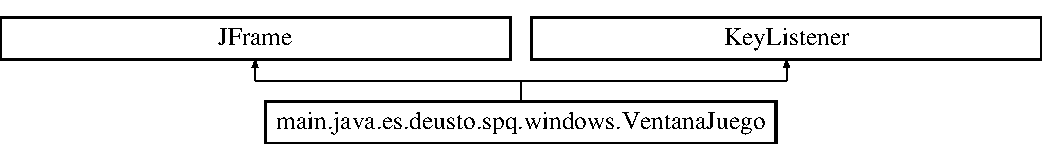
\includegraphics[height=1.911263cm]{classmain_1_1java_1_1es_1_1deusto_1_1spq_1_1windows_1_1_ventana_juego}
\end{center}
\end{figure}
\subsection*{Classes}
\begin{DoxyCompactItemize}
\item 
class {\bfseries Bajar\+Bloque}
\item 
class {\bfseries Bajar\+Ultimo\+Bloque}
\end{DoxyCompactItemize}
\subsection*{Public Member Functions}
\begin{DoxyCompactItemize}
\item 
\hyperlink{classmain_1_1java_1_1es_1_1deusto_1_1spq_1_1windows_1_1_ventana_juego_a833609fce8caed610b70524b8ce084bf}{Ventana\+Juego} (String titulo)
\item 
void \hyperlink{classmain_1_1java_1_1es_1_1deusto_1_1spq_1_1windows_1_1_ventana_juego_a325da4c37e78002e4326c5124f6a5fc5}{mover\+Bloque} (\hyperlink{classmain_1_1java_1_1es_1_1deusto_1_1spq_1_1data_1_1_bloque_grafico}{Bloque\+Grafico} bg)
\item 
void \hyperlink{classmain_1_1java_1_1es_1_1deusto_1_1spq_1_1windows_1_1_ventana_juego_ab157fd35f3fdf2c96f75e15709856e6a}{quitar\+Bloque} (\hyperlink{classmain_1_1java_1_1es_1_1deusto_1_1spq_1_1data_1_1_bloque_grafico}{Bloque\+Grafico} bg)
\item 
void \hyperlink{classmain_1_1java_1_1es_1_1deusto_1_1spq_1_1windows_1_1_ventana_juego_a90d331448fab674e578eedefed060a35}{add\+Bloque} (final \hyperlink{classmain_1_1java_1_1es_1_1deusto_1_1spq_1_1data_1_1_bloque_grafico}{Bloque\+Grafico} bg)
\item 
void \hyperlink{classmain_1_1java_1_1es_1_1deusto_1_1spq_1_1windows_1_1_ventana_juego_aac0f0bd3f21919ad6438f0c0c02497a8}{add\+Nave} (final \hyperlink{classmain_1_1java_1_1es_1_1deusto_1_1spq_1_1data_1_1_nave}{Nave} \hyperlink{classmain_1_1java_1_1es_1_1deusto_1_1spq_1_1windows_1_1_ventana_juego_a3e59bf8641104a1a8224d7def9866ead}{nv})
\item 
void \hyperlink{classmain_1_1java_1_1es_1_1deusto_1_1spq_1_1windows_1_1_ventana_juego_a2a3af9abbc02ea9b2b87cb87c30725bc}{mover\+Izquierda} ()
\item 
void \hyperlink{classmain_1_1java_1_1es_1_1deusto_1_1spq_1_1windows_1_1_ventana_juego_a4cc6b6ffb77ae2ba9a89cb18fe020e4c}{mover\+Derecha} ()
\item 
void \hyperlink{classmain_1_1java_1_1es_1_1deusto_1_1spq_1_1windows_1_1_ventana_juego_a6b215785ca3eaec27e8310989eaa5d9a}{suma\+Puntos} (\hyperlink{classmain_1_1java_1_1es_1_1deusto_1_1spq_1_1data_1_1_bloque_grafico}{Bloque\+Grafico} bg)
\item 
void \hyperlink{classmain_1_1java_1_1es_1_1deusto_1_1spq_1_1windows_1_1_ventana_juego_ad65c27316b3297db27f8dc3f3f6ae701}{key\+Pressed} (Key\+Event arg0)
\item 
void \hyperlink{classmain_1_1java_1_1es_1_1deusto_1_1spq_1_1windows_1_1_ventana_juego_ac5ce1d9ce49c1a312b0bebe279a1adec}{key\+Released} (Key\+Event arg0)
\item 
void \hyperlink{classmain_1_1java_1_1es_1_1deusto_1_1spq_1_1windows_1_1_ventana_juego_a86ac378bce474baad7622fecaf8721c0}{key\+Typed} (Key\+Event arg0)
\end{DoxyCompactItemize}
\subsection*{Static Public Attributes}
\begin{DoxyCompactItemize}
\item 
static \hyperlink{classmain_1_1java_1_1es_1_1deusto_1_1spq_1_1data_1_1_nave}{Nave} \hyperlink{classmain_1_1java_1_1es_1_1deusto_1_1spq_1_1windows_1_1_ventana_juego_a3e59bf8641104a1a8224d7def9866ead}{nv}
\end{DoxyCompactItemize}


\subsection{Detailed Description}
Creaci�n de la ventana de juego con el funcionamiento del juego principal \begin{DoxyAuthor}{Author}
001 
\end{DoxyAuthor}


Definition at line 32 of file Ventana\+Juego.\+java.



\subsection{Constructor \& Destructor Documentation}
\index{main\+::java\+::es\+::deusto\+::spq\+::windows\+::\+Ventana\+Juego@{main\+::java\+::es\+::deusto\+::spq\+::windows\+::\+Ventana\+Juego}!Ventana\+Juego@{Ventana\+Juego}}
\index{Ventana\+Juego@{Ventana\+Juego}!main\+::java\+::es\+::deusto\+::spq\+::windows\+::\+Ventana\+Juego@{main\+::java\+::es\+::deusto\+::spq\+::windows\+::\+Ventana\+Juego}}
\subsubsection[{\texorpdfstring{Ventana\+Juego(\+String titulo)}{VentanaJuego(String titulo)}}]{\setlength{\rightskip}{0pt plus 5cm}main.\+java.\+es.\+deusto.\+spq.\+windows.\+Ventana\+Juego.\+Ventana\+Juego (
\begin{DoxyParamCaption}
\item[{String}]{titulo}
\end{DoxyParamCaption}
)}\hypertarget{classmain_1_1java_1_1es_1_1deusto_1_1spq_1_1windows_1_1_ventana_juego_a833609fce8caed610b70524b8ce084bf}{}\label{classmain_1_1java_1_1es_1_1deusto_1_1spq_1_1windows_1_1_ventana_juego_a833609fce8caed610b70524b8ce084bf}
Constructor de la ventana de juego 

Definition at line 46 of file Ventana\+Juego.\+java.



\subsection{Member Function Documentation}
\index{main\+::java\+::es\+::deusto\+::spq\+::windows\+::\+Ventana\+Juego@{main\+::java\+::es\+::deusto\+::spq\+::windows\+::\+Ventana\+Juego}!add\+Bloque@{add\+Bloque}}
\index{add\+Bloque@{add\+Bloque}!main\+::java\+::es\+::deusto\+::spq\+::windows\+::\+Ventana\+Juego@{main\+::java\+::es\+::deusto\+::spq\+::windows\+::\+Ventana\+Juego}}
\subsubsection[{\texorpdfstring{add\+Bloque(final Bloque\+Grafico bg)}{addBloque(final BloqueGrafico bg)}}]{\setlength{\rightskip}{0pt plus 5cm}void main.\+java.\+es.\+deusto.\+spq.\+windows.\+Ventana\+Juego.\+add\+Bloque (
\begin{DoxyParamCaption}
\item[{final {\bf Bloque\+Grafico}}]{bg}
\end{DoxyParamCaption}
)}\hypertarget{classmain_1_1java_1_1es_1_1deusto_1_1spq_1_1windows_1_1_ventana_juego_a90d331448fab674e578eedefed060a35}{}\label{classmain_1_1java_1_1es_1_1deusto_1_1spq_1_1windows_1_1_ventana_juego_a90d331448fab674e578eedefed060a35}
A�ade a la ventana un bloque gr�fico, que se visualizar� inmediatamente si est� marcado para ser visible. 
\begin{DoxyParams}{Parameters}
{\em bg} & bloque gr�fico a introducir \\
\hline
\end{DoxyParams}


Definition at line 207 of file Ventana\+Juego.\+java.

\index{main\+::java\+::es\+::deusto\+::spq\+::windows\+::\+Ventana\+Juego@{main\+::java\+::es\+::deusto\+::spq\+::windows\+::\+Ventana\+Juego}!add\+Nave@{add\+Nave}}
\index{add\+Nave@{add\+Nave}!main\+::java\+::es\+::deusto\+::spq\+::windows\+::\+Ventana\+Juego@{main\+::java\+::es\+::deusto\+::spq\+::windows\+::\+Ventana\+Juego}}
\subsubsection[{\texorpdfstring{add\+Nave(final Nave nv)}{addNave(final Nave nv)}}]{\setlength{\rightskip}{0pt plus 5cm}void main.\+java.\+es.\+deusto.\+spq.\+windows.\+Ventana\+Juego.\+add\+Nave (
\begin{DoxyParamCaption}
\item[{final {\bf Nave}}]{nv}
\end{DoxyParamCaption}
)}\hypertarget{classmain_1_1java_1_1es_1_1deusto_1_1spq_1_1windows_1_1_ventana_juego_aac0f0bd3f21919ad6438f0c0c02497a8}{}\label{classmain_1_1java_1_1es_1_1deusto_1_1spq_1_1windows_1_1_ventana_juego_aac0f0bd3f21919ad6438f0c0c02497a8}
A�ade la nave de juego en la ventana 
\begin{DoxyParams}{Parameters}
{\em nv} & nave de juego a a�adir \\
\hline
\end{DoxyParams}


Definition at line 217 of file Ventana\+Juego.\+java.

\index{main\+::java\+::es\+::deusto\+::spq\+::windows\+::\+Ventana\+Juego@{main\+::java\+::es\+::deusto\+::spq\+::windows\+::\+Ventana\+Juego}!key\+Pressed@{key\+Pressed}}
\index{key\+Pressed@{key\+Pressed}!main\+::java\+::es\+::deusto\+::spq\+::windows\+::\+Ventana\+Juego@{main\+::java\+::es\+::deusto\+::spq\+::windows\+::\+Ventana\+Juego}}
\subsubsection[{\texorpdfstring{key\+Pressed(\+Key\+Event arg0)}{keyPressed(KeyEvent arg0)}}]{\setlength{\rightskip}{0pt plus 5cm}void main.\+java.\+es.\+deusto.\+spq.\+windows.\+Ventana\+Juego.\+key\+Pressed (
\begin{DoxyParamCaption}
\item[{Key\+Event}]{arg0}
\end{DoxyParamCaption}
)}\hypertarget{classmain_1_1java_1_1es_1_1deusto_1_1spq_1_1windows_1_1_ventana_juego_ad65c27316b3297db27f8dc3f3f6ae701}{}\label{classmain_1_1java_1_1es_1_1deusto_1_1spq_1_1windows_1_1_ventana_juego_ad65c27316b3297db27f8dc3f3f6ae701}


Definition at line 258 of file Ventana\+Juego.\+java.

\index{main\+::java\+::es\+::deusto\+::spq\+::windows\+::\+Ventana\+Juego@{main\+::java\+::es\+::deusto\+::spq\+::windows\+::\+Ventana\+Juego}!key\+Released@{key\+Released}}
\index{key\+Released@{key\+Released}!main\+::java\+::es\+::deusto\+::spq\+::windows\+::\+Ventana\+Juego@{main\+::java\+::es\+::deusto\+::spq\+::windows\+::\+Ventana\+Juego}}
\subsubsection[{\texorpdfstring{key\+Released(\+Key\+Event arg0)}{keyReleased(KeyEvent arg0)}}]{\setlength{\rightskip}{0pt plus 5cm}void main.\+java.\+es.\+deusto.\+spq.\+windows.\+Ventana\+Juego.\+key\+Released (
\begin{DoxyParamCaption}
\item[{Key\+Event}]{arg0}
\end{DoxyParamCaption}
)}\hypertarget{classmain_1_1java_1_1es_1_1deusto_1_1spq_1_1windows_1_1_ventana_juego_ac5ce1d9ce49c1a312b0bebe279a1adec}{}\label{classmain_1_1java_1_1es_1_1deusto_1_1spq_1_1windows_1_1_ventana_juego_ac5ce1d9ce49c1a312b0bebe279a1adec}


Definition at line 271 of file Ventana\+Juego.\+java.

\index{main\+::java\+::es\+::deusto\+::spq\+::windows\+::\+Ventana\+Juego@{main\+::java\+::es\+::deusto\+::spq\+::windows\+::\+Ventana\+Juego}!key\+Typed@{key\+Typed}}
\index{key\+Typed@{key\+Typed}!main\+::java\+::es\+::deusto\+::spq\+::windows\+::\+Ventana\+Juego@{main\+::java\+::es\+::deusto\+::spq\+::windows\+::\+Ventana\+Juego}}
\subsubsection[{\texorpdfstring{key\+Typed(\+Key\+Event arg0)}{keyTyped(KeyEvent arg0)}}]{\setlength{\rightskip}{0pt plus 5cm}void main.\+java.\+es.\+deusto.\+spq.\+windows.\+Ventana\+Juego.\+key\+Typed (
\begin{DoxyParamCaption}
\item[{Key\+Event}]{arg0}
\end{DoxyParamCaption}
)}\hypertarget{classmain_1_1java_1_1es_1_1deusto_1_1spq_1_1windows_1_1_ventana_juego_a86ac378bce474baad7622fecaf8721c0}{}\label{classmain_1_1java_1_1es_1_1deusto_1_1spq_1_1windows_1_1_ventana_juego_a86ac378bce474baad7622fecaf8721c0}


Definition at line 276 of file Ventana\+Juego.\+java.

\index{main\+::java\+::es\+::deusto\+::spq\+::windows\+::\+Ventana\+Juego@{main\+::java\+::es\+::deusto\+::spq\+::windows\+::\+Ventana\+Juego}!mover\+Bloque@{mover\+Bloque}}
\index{mover\+Bloque@{mover\+Bloque}!main\+::java\+::es\+::deusto\+::spq\+::windows\+::\+Ventana\+Juego@{main\+::java\+::es\+::deusto\+::spq\+::windows\+::\+Ventana\+Juego}}
\subsubsection[{\texorpdfstring{mover\+Bloque(\+Bloque\+Grafico bg)}{moverBloque(BloqueGrafico bg)}}]{\setlength{\rightskip}{0pt plus 5cm}void main.\+java.\+es.\+deusto.\+spq.\+windows.\+Ventana\+Juego.\+mover\+Bloque (
\begin{DoxyParamCaption}
\item[{{\bf Bloque\+Grafico}}]{bg}
\end{DoxyParamCaption}
)}\hypertarget{classmain_1_1java_1_1es_1_1deusto_1_1spq_1_1windows_1_1_ventana_juego_a325da4c37e78002e4326c5124f6a5fc5}{}\label{classmain_1_1java_1_1es_1_1deusto_1_1spq_1_1windows_1_1_ventana_juego_a325da4c37e78002e4326c5124f6a5fc5}
M�todo para mover un bloque gr�fico hasta cierta altura Desaparece al llegar abajo o al chocar con la nave 
\begin{DoxyParams}{Parameters}
{\em bg} & bloque gr�fico a mover \\
\hline
\end{DoxyParams}


Definition at line 175 of file Ventana\+Juego.\+java.

\index{main\+::java\+::es\+::deusto\+::spq\+::windows\+::\+Ventana\+Juego@{main\+::java\+::es\+::deusto\+::spq\+::windows\+::\+Ventana\+Juego}!mover\+Derecha@{mover\+Derecha}}
\index{mover\+Derecha@{mover\+Derecha}!main\+::java\+::es\+::deusto\+::spq\+::windows\+::\+Ventana\+Juego@{main\+::java\+::es\+::deusto\+::spq\+::windows\+::\+Ventana\+Juego}}
\subsubsection[{\texorpdfstring{mover\+Derecha()}{moverDerecha()}}]{\setlength{\rightskip}{0pt plus 5cm}void main.\+java.\+es.\+deusto.\+spq.\+windows.\+Ventana\+Juego.\+mover\+Derecha (
\begin{DoxyParamCaption}
{}
\end{DoxyParamCaption}
)}\hypertarget{classmain_1_1java_1_1es_1_1deusto_1_1spq_1_1windows_1_1_ventana_juego_a4cc6b6ffb77ae2ba9a89cb18fe020e4c}{}\label{classmain_1_1java_1_1es_1_1deusto_1_1spq_1_1windows_1_1_ventana_juego_a4cc6b6ffb77ae2ba9a89cb18fe020e4c}
Desplaza la nave a la siguiente posici�n a la derecha 

Definition at line 237 of file Ventana\+Juego.\+java.

\index{main\+::java\+::es\+::deusto\+::spq\+::windows\+::\+Ventana\+Juego@{main\+::java\+::es\+::deusto\+::spq\+::windows\+::\+Ventana\+Juego}!mover\+Izquierda@{mover\+Izquierda}}
\index{mover\+Izquierda@{mover\+Izquierda}!main\+::java\+::es\+::deusto\+::spq\+::windows\+::\+Ventana\+Juego@{main\+::java\+::es\+::deusto\+::spq\+::windows\+::\+Ventana\+Juego}}
\subsubsection[{\texorpdfstring{mover\+Izquierda()}{moverIzquierda()}}]{\setlength{\rightskip}{0pt plus 5cm}void main.\+java.\+es.\+deusto.\+spq.\+windows.\+Ventana\+Juego.\+mover\+Izquierda (
\begin{DoxyParamCaption}
{}
\end{DoxyParamCaption}
)}\hypertarget{classmain_1_1java_1_1es_1_1deusto_1_1spq_1_1windows_1_1_ventana_juego_a2a3af9abbc02ea9b2b87cb87c30725bc}{}\label{classmain_1_1java_1_1es_1_1deusto_1_1spq_1_1windows_1_1_ventana_juego_a2a3af9abbc02ea9b2b87cb87c30725bc}
Desplaza la nave a la siguiente posici�n a la izquierda 

Definition at line 226 of file Ventana\+Juego.\+java.

\index{main\+::java\+::es\+::deusto\+::spq\+::windows\+::\+Ventana\+Juego@{main\+::java\+::es\+::deusto\+::spq\+::windows\+::\+Ventana\+Juego}!quitar\+Bloque@{quitar\+Bloque}}
\index{quitar\+Bloque@{quitar\+Bloque}!main\+::java\+::es\+::deusto\+::spq\+::windows\+::\+Ventana\+Juego@{main\+::java\+::es\+::deusto\+::spq\+::windows\+::\+Ventana\+Juego}}
\subsubsection[{\texorpdfstring{quitar\+Bloque(\+Bloque\+Grafico bg)}{quitarBloque(BloqueGrafico bg)}}]{\setlength{\rightskip}{0pt plus 5cm}void main.\+java.\+es.\+deusto.\+spq.\+windows.\+Ventana\+Juego.\+quitar\+Bloque (
\begin{DoxyParamCaption}
\item[{{\bf Bloque\+Grafico}}]{bg}
\end{DoxyParamCaption}
)}\hypertarget{classmain_1_1java_1_1es_1_1deusto_1_1spq_1_1windows_1_1_ventana_juego_ab157fd35f3fdf2c96f75e15709856e6a}{}\label{classmain_1_1java_1_1es_1_1deusto_1_1spq_1_1windows_1_1_ventana_juego_ab157fd35f3fdf2c96f75e15709856e6a}
M�todo para eliminar un bloque gr�fico 
\begin{DoxyParams}{Parameters}
{\em bg} & bloque gr�fico a eliminar \\
\hline
\end{DoxyParams}


Definition at line 198 of file Ventana\+Juego.\+java.

\index{main\+::java\+::es\+::deusto\+::spq\+::windows\+::\+Ventana\+Juego@{main\+::java\+::es\+::deusto\+::spq\+::windows\+::\+Ventana\+Juego}!suma\+Puntos@{suma\+Puntos}}
\index{suma\+Puntos@{suma\+Puntos}!main\+::java\+::es\+::deusto\+::spq\+::windows\+::\+Ventana\+Juego@{main\+::java\+::es\+::deusto\+::spq\+::windows\+::\+Ventana\+Juego}}
\subsubsection[{\texorpdfstring{suma\+Puntos(\+Bloque\+Grafico bg)}{sumaPuntos(BloqueGrafico bg)}}]{\setlength{\rightskip}{0pt plus 5cm}void main.\+java.\+es.\+deusto.\+spq.\+windows.\+Ventana\+Juego.\+suma\+Puntos (
\begin{DoxyParamCaption}
\item[{{\bf Bloque\+Grafico}}]{bg}
\end{DoxyParamCaption}
)}\hypertarget{classmain_1_1java_1_1es_1_1deusto_1_1spq_1_1windows_1_1_ventana_juego_a6b215785ca3eaec27e8310989eaa5d9a}{}\label{classmain_1_1java_1_1es_1_1deusto_1_1spq_1_1windows_1_1_ventana_juego_a6b215785ca3eaec27e8310989eaa5d9a}
Lleva la cuenta de los puntos de la partida Los bloques de color suman 10, los grises restan 10 
\begin{DoxyParams}{Parameters}
{\em bg} & \\
\hline
\end{DoxyParams}


Definition at line 250 of file Ventana\+Juego.\+java.



\subsection{Member Data Documentation}
\index{main\+::java\+::es\+::deusto\+::spq\+::windows\+::\+Ventana\+Juego@{main\+::java\+::es\+::deusto\+::spq\+::windows\+::\+Ventana\+Juego}!nv@{nv}}
\index{nv@{nv}!main\+::java\+::es\+::deusto\+::spq\+::windows\+::\+Ventana\+Juego@{main\+::java\+::es\+::deusto\+::spq\+::windows\+::\+Ventana\+Juego}}
\subsubsection[{\texorpdfstring{nv}{nv}}]{\setlength{\rightskip}{0pt plus 5cm}{\bf Nave} main.\+java.\+es.\+deusto.\+spq.\+windows.\+Ventana\+Juego.\+nv\hspace{0.3cm}{\ttfamily [static]}}\hypertarget{classmain_1_1java_1_1es_1_1deusto_1_1spq_1_1windows_1_1_ventana_juego_a3e59bf8641104a1a8224d7def9866ead}{}\label{classmain_1_1java_1_1es_1_1deusto_1_1spq_1_1windows_1_1_ventana_juego_a3e59bf8641104a1a8224d7def9866ead}


Definition at line 36 of file Ventana\+Juego.\+java.



The documentation for this class was generated from the following file\+:\begin{DoxyCompactItemize}
\item 
src/main/java/es/deusto/spq/windows/\hyperlink{_ventana_juego_8java}{Ventana\+Juego.\+java}\end{DoxyCompactItemize}

\hypertarget{classmain_1_1java_1_1es_1_1deusto_1_1spq_1_1windows_1_1_ventana_seleccion_cancion}{}\section{main.\+java.\+es.\+deusto.\+spq.\+windows.\+Ventana\+Seleccion\+Cancion Class Reference}
\label{classmain_1_1java_1_1es_1_1deusto_1_1spq_1_1windows_1_1_ventana_seleccion_cancion}\index{main.\+java.\+es.\+deusto.\+spq.\+windows.\+Ventana\+Seleccion\+Cancion@{main.\+java.\+es.\+deusto.\+spq.\+windows.\+Ventana\+Seleccion\+Cancion}}
Inheritance diagram for main.\+java.\+es.\+deusto.\+spq.\+windows.\+Ventana\+Seleccion\+Cancion\+:\begin{figure}[H]
\begin{center}
\leavevmode
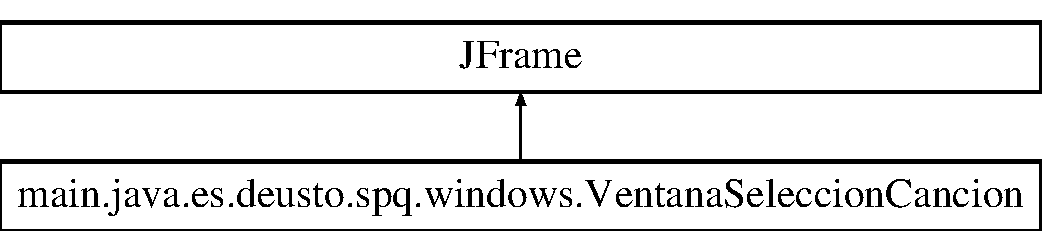
\includegraphics[height=2.000000cm]{classmain_1_1java_1_1es_1_1deusto_1_1spq_1_1windows_1_1_ventana_seleccion_cancion}
\end{center}
\end{figure}
\subsection*{Public Member Functions}
\begin{DoxyCompactItemize}
\item 
\hyperlink{classmain_1_1java_1_1es_1_1deusto_1_1spq_1_1windows_1_1_ventana_seleccion_cancion_ad8166ac2780667cca7441ef4f5bd4c14}{Ventana\+Seleccion\+Cancion} ()
\end{DoxyCompactItemize}


\subsection{Detailed Description}
Ventana para elegir la canci�n que se va a jugar \begin{DoxyAuthor}{Author}
001 
\end{DoxyAuthor}


Definition at line 22 of file Ventana\+Seleccion\+Cancion.\+java.



\subsection{Constructor \& Destructor Documentation}
\index{main\+::java\+::es\+::deusto\+::spq\+::windows\+::\+Ventana\+Seleccion\+Cancion@{main\+::java\+::es\+::deusto\+::spq\+::windows\+::\+Ventana\+Seleccion\+Cancion}!Ventana\+Seleccion\+Cancion@{Ventana\+Seleccion\+Cancion}}
\index{Ventana\+Seleccion\+Cancion@{Ventana\+Seleccion\+Cancion}!main\+::java\+::es\+::deusto\+::spq\+::windows\+::\+Ventana\+Seleccion\+Cancion@{main\+::java\+::es\+::deusto\+::spq\+::windows\+::\+Ventana\+Seleccion\+Cancion}}
\subsubsection[{\texorpdfstring{Ventana\+Seleccion\+Cancion()}{VentanaSeleccionCancion()}}]{\setlength{\rightskip}{0pt plus 5cm}main.\+java.\+es.\+deusto.\+spq.\+windows.\+Ventana\+Seleccion\+Cancion.\+Ventana\+Seleccion\+Cancion (
\begin{DoxyParamCaption}
{}
\end{DoxyParamCaption}
)}\hypertarget{classmain_1_1java_1_1es_1_1deusto_1_1spq_1_1windows_1_1_ventana_seleccion_cancion_ad8166ac2780667cca7441ef4f5bd4c14}{}\label{classmain_1_1java_1_1es_1_1deusto_1_1spq_1_1windows_1_1_ventana_seleccion_cancion_ad8166ac2780667cca7441ef4f5bd4c14}
Constructor de la ventana de selecci�n de canci�n 

Definition at line 34 of file Ventana\+Seleccion\+Cancion.\+java.



The documentation for this class was generated from the following file\+:\begin{DoxyCompactItemize}
\item 
src/main/java/es/deusto/spq/windows/\hyperlink{_ventana_seleccion_cancion_8java}{Ventana\+Seleccion\+Cancion.\+java}\end{DoxyCompactItemize}

\chapter{File Documentation}
\hypertarget{_bloque_8java}{}\section{src/main/java/es/deusto/spq/data/\+Bloque.java File Reference}
\label{_bloque_8java}\index{src/main/java/es/deusto/spq/data/\+Bloque.\+java@{src/main/java/es/deusto/spq/data/\+Bloque.\+java}}
\subsection*{Classes}
\begin{DoxyCompactItemize}
\item 
class \hyperlink{classmain_1_1java_1_1es_1_1deusto_1_1spq_1_1data_1_1_bloque}{main.\+java.\+es.\+deusto.\+spq.\+data.\+Bloque}
\item 
enum \hyperlink{enummain_1_1java_1_1es_1_1deusto_1_1spq_1_1data_1_1_bloque_1_1_tipo}{main.\+java.\+es.\+deusto.\+spq.\+data.\+Bloque.\+Tipo}
\end{DoxyCompactItemize}
\subsection*{Packages}
\begin{DoxyCompactItemize}
\item 
package \hyperlink{namespacemain_1_1java_1_1es_1_1deusto_1_1spq_1_1data}{main.\+java.\+es.\+deusto.\+spq.\+data}
\end{DoxyCompactItemize}

\hypertarget{_bloque_grafico_8java}{}\section{src/main/java/es/deusto/spq/data/\+Bloque\+Grafico.java File Reference}
\label{_bloque_grafico_8java}\index{src/main/java/es/deusto/spq/data/\+Bloque\+Grafico.\+java@{src/main/java/es/deusto/spq/data/\+Bloque\+Grafico.\+java}}
\subsection*{Classes}
\begin{DoxyCompactItemize}
\item 
class \hyperlink{classmain_1_1java_1_1es_1_1deusto_1_1spq_1_1data_1_1_bloque_grafico}{main.\+java.\+es.\+deusto.\+spq.\+data.\+Bloque\+Grafico}
\end{DoxyCompactItemize}
\subsection*{Packages}
\begin{DoxyCompactItemize}
\item 
package \hyperlink{namespacemain_1_1java_1_1es_1_1deusto_1_1spq_1_1data}{main.\+java.\+es.\+deusto.\+spq.\+data}
\end{DoxyCompactItemize}

\hypertarget{_cancion_8java}{}\section{src/main/java/es/deusto/spq/data/\+Cancion.java File Reference}
\label{_cancion_8java}\index{src/main/java/es/deusto/spq/data/\+Cancion.\+java@{src/main/java/es/deusto/spq/data/\+Cancion.\+java}}
\subsection*{Classes}
\begin{DoxyCompactItemize}
\item 
class \hyperlink{classmain_1_1java_1_1es_1_1deusto_1_1spq_1_1data_1_1_cancion}{main.\+java.\+es.\+deusto.\+spq.\+data.\+Cancion}
\end{DoxyCompactItemize}
\subsection*{Packages}
\begin{DoxyCompactItemize}
\item 
package \hyperlink{namespacemain_1_1java_1_1es_1_1deusto_1_1spq_1_1data}{main.\+java.\+es.\+deusto.\+spq.\+data}
\end{DoxyCompactItemize}

\hypertarget{_nave_8java}{}\section{src/main/java/es/deusto/spq/data/\+Nave.java File Reference}
\label{_nave_8java}\index{src/main/java/es/deusto/spq/data/\+Nave.\+java@{src/main/java/es/deusto/spq/data/\+Nave.\+java}}
\subsection*{Classes}
\begin{DoxyCompactItemize}
\item 
class \hyperlink{classmain_1_1java_1_1es_1_1deusto_1_1spq_1_1data_1_1_nave}{main.\+java.\+es.\+deusto.\+spq.\+data.\+Nave}
\end{DoxyCompactItemize}
\subsection*{Packages}
\begin{DoxyCompactItemize}
\item 
package \hyperlink{namespacemain_1_1java_1_1es_1_1deusto_1_1spq_1_1data}{main.\+java.\+es.\+deusto.\+spq.\+data}
\end{DoxyCompactItemize}

\hypertarget{_reproducir_canciones_8java}{}\section{src/main/java/es/deusto/spq/data/\+Reproducir\+Canciones.java File Reference}
\label{_reproducir_canciones_8java}\index{src/main/java/es/deusto/spq/data/\+Reproducir\+Canciones.\+java@{src/main/java/es/deusto/spq/data/\+Reproducir\+Canciones.\+java}}
\subsection*{Classes}
\begin{DoxyCompactItemize}
\item 
class \hyperlink{classmain_1_1java_1_1es_1_1deusto_1_1spq_1_1data_1_1_reproducir_canciones}{main.\+java.\+es.\+deusto.\+spq.\+data.\+Reproducir\+Canciones}
\end{DoxyCompactItemize}
\subsection*{Packages}
\begin{DoxyCompactItemize}
\item 
package \hyperlink{namespacemain_1_1java_1_1es_1_1deusto_1_1spq_1_1data}{main.\+java.\+es.\+deusto.\+spq.\+data}
\end{DoxyCompactItemize}

\hypertarget{_b_d_8java}{}\section{src/main/java/es/deusto/spq/utils/\+BD.java File Reference}
\label{_b_d_8java}\index{src/main/java/es/deusto/spq/utils/\+B\+D.\+java@{src/main/java/es/deusto/spq/utils/\+B\+D.\+java}}
\subsection*{Classes}
\begin{DoxyCompactItemize}
\item 
class \hyperlink{classmain_1_1java_1_1es_1_1deusto_1_1spq_1_1utils_1_1_b_d}{main.\+java.\+es.\+deusto.\+spq.\+utils.\+BD}
\end{DoxyCompactItemize}
\subsection*{Packages}
\begin{DoxyCompactItemize}
\item 
package \hyperlink{namespacemain_1_1java_1_1es_1_1deusto_1_1spq_1_1utils}{main.\+java.\+es.\+deusto.\+spq.\+utils}
\end{DoxyCompactItemize}

\hypertarget{_file_manager_8java}{}\section{src/main/java/es/deusto/spq/utils/\+File\+Manager.java File Reference}
\label{_file_manager_8java}\index{src/main/java/es/deusto/spq/utils/\+File\+Manager.\+java@{src/main/java/es/deusto/spq/utils/\+File\+Manager.\+java}}
\subsection*{Classes}
\begin{DoxyCompactItemize}
\item 
class \hyperlink{classmain_1_1java_1_1es_1_1deusto_1_1spq_1_1utils_1_1_file_manager}{main.\+java.\+es.\+deusto.\+spq.\+utils.\+File\+Manager}
\end{DoxyCompactItemize}
\subsection*{Packages}
\begin{DoxyCompactItemize}
\item 
package \hyperlink{namespacemain_1_1java_1_1es_1_1deusto_1_1spq_1_1utils}{main.\+java.\+es.\+deusto.\+spq.\+utils}
\end{DoxyCompactItemize}

\hypertarget{_menu_window_8java}{}\section{src/main/java/es/deusto/spq/windows/\+Menu\+Window.java File Reference}
\label{_menu_window_8java}\index{src/main/java/es/deusto/spq/windows/\+Menu\+Window.\+java@{src/main/java/es/deusto/spq/windows/\+Menu\+Window.\+java}}
\subsection*{Classes}
\begin{DoxyCompactItemize}
\item 
class \hyperlink{classmain_1_1java_1_1es_1_1deusto_1_1spq_1_1windows_1_1_menu_window}{main.\+java.\+es.\+deusto.\+spq.\+windows.\+Menu\+Window}
\item 
class {\bfseries main.\+java.\+es.\+deusto.\+spq.\+windows.\+Menu\+Window.\+Quit}
\end{DoxyCompactItemize}
\subsection*{Packages}
\begin{DoxyCompactItemize}
\item 
package \hyperlink{namespacemain_1_1java_1_1es_1_1deusto_1_1spq_1_1windows}{main.\+java.\+es.\+deusto.\+spq.\+windows}
\end{DoxyCompactItemize}

\hypertarget{_objeto_grafico_8java}{}\section{src/main/java/es/deusto/spq/windows/\+Objeto\+Grafico.java File Reference}
\label{_objeto_grafico_8java}\index{src/main/java/es/deusto/spq/windows/\+Objeto\+Grafico.\+java@{src/main/java/es/deusto/spq/windows/\+Objeto\+Grafico.\+java}}
\subsection*{Classes}
\begin{DoxyCompactItemize}
\item 
class \hyperlink{classmain_1_1java_1_1es_1_1deusto_1_1spq_1_1windows_1_1_objeto_grafico}{main.\+java.\+es.\+deusto.\+spq.\+windows.\+Objeto\+Grafico}
\end{DoxyCompactItemize}
\subsection*{Packages}
\begin{DoxyCompactItemize}
\item 
package \hyperlink{namespacemain_1_1java_1_1es_1_1deusto_1_1spq_1_1windows}{main.\+java.\+es.\+deusto.\+spq.\+windows}
\end{DoxyCompactItemize}

\hypertarget{_ventana_editor_8java}{}\section{src/main/java/es/deusto/spq/windows/\+Ventana\+Editor.java File Reference}
\label{_ventana_editor_8java}\index{src/main/java/es/deusto/spq/windows/\+Ventana\+Editor.\+java@{src/main/java/es/deusto/spq/windows/\+Ventana\+Editor.\+java}}
\subsection*{Classes}
\begin{DoxyCompactItemize}
\item 
class \hyperlink{classmain_1_1java_1_1es_1_1deusto_1_1spq_1_1windows_1_1_ventana_editor}{main.\+java.\+es.\+deusto.\+spq.\+windows.\+Ventana\+Editor}
\end{DoxyCompactItemize}
\subsection*{Packages}
\begin{DoxyCompactItemize}
\item 
package \hyperlink{namespacemain_1_1java_1_1es_1_1deusto_1_1spq_1_1windows}{main.\+java.\+es.\+deusto.\+spq.\+windows}
\end{DoxyCompactItemize}

\hypertarget{_ventana_juego_8java}{}\section{src/main/java/es/deusto/spq/windows/\+Ventana\+Juego.java File Reference}
\label{_ventana_juego_8java}\index{src/main/java/es/deusto/spq/windows/\+Ventana\+Juego.\+java@{src/main/java/es/deusto/spq/windows/\+Ventana\+Juego.\+java}}
\subsection*{Classes}
\begin{DoxyCompactItemize}
\item 
class \hyperlink{classmain_1_1java_1_1es_1_1deusto_1_1spq_1_1windows_1_1_ventana_juego}{main.\+java.\+es.\+deusto.\+spq.\+windows.\+Ventana\+Juego}
\item 
class {\bfseries main.\+java.\+es.\+deusto.\+spq.\+windows.\+Ventana\+Juego.\+Bajar\+Bloque}
\item 
class {\bfseries main.\+java.\+es.\+deusto.\+spq.\+windows.\+Ventana\+Juego.\+Bajar\+Ultimo\+Bloque}
\end{DoxyCompactItemize}
\subsection*{Packages}
\begin{DoxyCompactItemize}
\item 
package \hyperlink{namespacemain_1_1java_1_1es_1_1deusto_1_1spq_1_1windows}{main.\+java.\+es.\+deusto.\+spq.\+windows}
\end{DoxyCompactItemize}

\hypertarget{_ventana_seleccion_cancion_8java}{}\section{src/main/java/es/deusto/spq/windows/\+Ventana\+Seleccion\+Cancion.java File Reference}
\label{_ventana_seleccion_cancion_8java}\index{src/main/java/es/deusto/spq/windows/\+Ventana\+Seleccion\+Cancion.\+java@{src/main/java/es/deusto/spq/windows/\+Ventana\+Seleccion\+Cancion.\+java}}
\subsection*{Classes}
\begin{DoxyCompactItemize}
\item 
class \hyperlink{classmain_1_1java_1_1es_1_1deusto_1_1spq_1_1windows_1_1_ventana_seleccion_cancion}{main.\+java.\+es.\+deusto.\+spq.\+windows.\+Ventana\+Seleccion\+Cancion}
\end{DoxyCompactItemize}
\subsection*{Packages}
\begin{DoxyCompactItemize}
\item 
package \hyperlink{namespacemain_1_1java_1_1es_1_1deusto_1_1spq_1_1windows}{main.\+java.\+es.\+deusto.\+spq.\+windows}
\end{DoxyCompactItemize}

\hypertarget{_test_bloque_8java}{}\section{src/test/java/es/deusto/spq/\+Test\+Bloque.java File Reference}
\label{_test_bloque_8java}\index{src/test/java/es/deusto/spq/\+Test\+Bloque.\+java@{src/test/java/es/deusto/spq/\+Test\+Bloque.\+java}}
\subsection*{Classes}
\begin{DoxyCompactItemize}
\item 
class \hyperlink{classtest_1_1java_1_1es_1_1deusto_1_1spq_1_1_test_bloque}{test.\+java.\+es.\+deusto.\+spq.\+Test\+Bloque}
\end{DoxyCompactItemize}
\subsection*{Packages}
\begin{DoxyCompactItemize}
\item 
package \hyperlink{namespacetest_1_1java_1_1es_1_1deusto_1_1spq}{test.\+java.\+es.\+deusto.\+spq}
\end{DoxyCompactItemize}

\hypertarget{_test_bloque_grafico_8java}{}\section{src/test/java/es/deusto/spq/\+Test\+Bloque\+Grafico.java File Reference}
\label{_test_bloque_grafico_8java}\index{src/test/java/es/deusto/spq/\+Test\+Bloque\+Grafico.\+java@{src/test/java/es/deusto/spq/\+Test\+Bloque\+Grafico.\+java}}
\subsection*{Classes}
\begin{DoxyCompactItemize}
\item 
class \hyperlink{classtest_1_1java_1_1es_1_1deusto_1_1spq_1_1_test_bloque_grafico}{test.\+java.\+es.\+deusto.\+spq.\+Test\+Bloque\+Grafico}
\end{DoxyCompactItemize}
\subsection*{Packages}
\begin{DoxyCompactItemize}
\item 
package \hyperlink{namespacetest_1_1java_1_1es_1_1deusto_1_1spq}{test.\+java.\+es.\+deusto.\+spq}
\end{DoxyCompactItemize}

\hypertarget{_test_mover_nave_8java}{}\section{src/test/java/es/deusto/spq/\+Test\+Mover\+Nave.java File Reference}
\label{_test_mover_nave_8java}\index{src/test/java/es/deusto/spq/\+Test\+Mover\+Nave.\+java@{src/test/java/es/deusto/spq/\+Test\+Mover\+Nave.\+java}}
\subsection*{Classes}
\begin{DoxyCompactItemize}
\item 
class \hyperlink{classtest_1_1java_1_1es_1_1deusto_1_1spq_1_1_test_mover_nave}{test.\+java.\+es.\+deusto.\+spq.\+Test\+Mover\+Nave}
\end{DoxyCompactItemize}
\subsection*{Packages}
\begin{DoxyCompactItemize}
\item 
package \hyperlink{namespacetest_1_1java_1_1es_1_1deusto_1_1spq}{test.\+java.\+es.\+deusto.\+spq}
\end{DoxyCompactItemize}

\hypertarget{_test_objeto_grafico_8java}{}\section{src/test/java/es/deusto/spq/\+Test\+Objeto\+Grafico.java File Reference}
\label{_test_objeto_grafico_8java}\index{src/test/java/es/deusto/spq/\+Test\+Objeto\+Grafico.\+java@{src/test/java/es/deusto/spq/\+Test\+Objeto\+Grafico.\+java}}
\subsection*{Classes}
\begin{DoxyCompactItemize}
\item 
class \hyperlink{classtest_1_1java_1_1es_1_1deusto_1_1spq_1_1_test_objeto_grafico}{test.\+java.\+es.\+deusto.\+spq.\+Test\+Objeto\+Grafico}
\end{DoxyCompactItemize}
\subsection*{Packages}
\begin{DoxyCompactItemize}
\item 
package \hyperlink{namespacetest_1_1java_1_1es_1_1deusto_1_1spq}{test.\+java.\+es.\+deusto.\+spq}
\end{DoxyCompactItemize}

\hypertarget{_test_ventana_juego_8java}{}\section{src/test/java/es/deusto/spq/\+Test\+Ventana\+Juego.java File Reference}
\label{_test_ventana_juego_8java}\index{src/test/java/es/deusto/spq/\+Test\+Ventana\+Juego.\+java@{src/test/java/es/deusto/spq/\+Test\+Ventana\+Juego.\+java}}
\subsection*{Classes}
\begin{DoxyCompactItemize}
\item 
class \hyperlink{classtest_1_1java_1_1es_1_1deusto_1_1spq_1_1_test_ventana_juego}{test.\+java.\+es.\+deusto.\+spq.\+Test\+Ventana\+Juego}
\end{DoxyCompactItemize}
\subsection*{Packages}
\begin{DoxyCompactItemize}
\item 
package \hyperlink{namespacetest_1_1java_1_1es_1_1deusto_1_1spq}{test.\+java.\+es.\+deusto.\+spq}
\end{DoxyCompactItemize}

%--- End generated contents ---

% Index
\backmatter
\newpage
\phantomsection
\clearemptydoublepage
\addcontentsline{toc}{chapter}{Index}
\printindex

\end{document}
